% RMIT University School of CS&IT
% Minor thesis template
% S.M.M. (Saied) Tahaghoghi, 2004

\documentclass[11pt,twoside]{report}
\usepackage{a4wide,caption,epsfig,fancyheadings,url}
\usepackage{subcaption}
\usepackage{graphicx}

\graphicspath{ {./Figs/} }
\setcounter{secnumdepth}{3}

% Place the correct values here
%Set to the original submission date when submitted amended thesis
\newcommand{\SubmissionDate}{\today}
\newcommand{\student}{Tyler Saxton}
\newcommand{\supervisor}{Dr. Dhirendra Singh}
\newcommand{\topic}{Mapping suburban bicycle lanes using street scene images and deep learning}
\newcommand{\school}{School of Computer Science and Information Technology}
\newcommand{\program}{Masters of Data Science}
\newcommand{\institution}{Royal Melbourne Institute of Technology}

% Use the remark command to highlight text for discussion
\newcommand{\remark}[1]{{\bf \em [\marginpar{$\Leftarrow$}#1]}}

\renewcommand{\leftmark}{\student}
\renewcommand{\rightmark}{\topic}
\renewcommand{\headrulewidth}{0pt}
\setlength{\parindent}{0pt}
\setlength{\parskip}{1.5ex plus 0.3ex}

% This is the line spacing - set to 2 for draft submission to
% supervisor, 1.3 for the final submission
\renewcommand{\baselinestretch}{1.3}

\renewcommand{\captionfont}{\it}
\raggedbottom

\begin{document}

%%%%%%%%%%%%%%%%%%%%%%%%%%%%%%%%%%%%%%%%%%%%%%%%%%%%%%%%%%%%%%%%%%%%%%
\title{{\Large\bf \topic}}
\author{
A minor thesis submitted in partial fulfilment of the requirements for the degree of
\\\program\\*[10mm]
%\epsfig{figure=Figs/rmit-coa.epsf,width=5cm}
\\\student
\\\school
\\Science, Engineering, and Technology Portfolio,
\\\institution
\\Melbourne, Victoria, Australia
}
\maketitle
\thispagestyle{empty}


%%%%%%%%%%%%%%%%%%%%%%%%%%%%%%%%%%%%%%%%%%%%%%%%%%%%%%%%%%%%%%%%%%%%%%
\chapter*{Declaration}

This thesis contains work that has not been submitted previously, in
whole or in part, for any other academic award and is solely my
original research, except where acknowledged.

This work has been carried out since March 2021, under the
supervision of {\supervisor}.

\paragraph{}
\vspace{5cm}\noindent \\\student \\
\school\\
\institution\\
\SubmissionDate

\pagenumbering{roman}


%%%%%%%%%%%%%%%%%%%%%%%%%%%%%%%%%%%%%%%%%%%%%%%%%%%%%%%%%%%%%%%%%%%%%%
\chapter*{Acknowledgements}

First and foremost, I would like to thank Dr. Dhirendra Singh for inspiring this research and supervising me throughout the year.  I also greatly appreciate the input provided by Dr. Ron van Schyndel and the ``Research Methods'' class of Semester 1 2021, as I worked to develop a detailed research proposal. \\

To Dr. Sophie Bittinger, Dr. Logan Bittinger, Laura Pritchard, and Dr. Curtis Saxton, thank you for your encouragement, and your assistance with the editing process.


%%%%%%%%%%%%%%%%%%%%%%%%%%%%%%%%%%%%%%%%%%%%%%%%%%%%%%%%%%%%%%%%%%%%%%
\chapter*{Summary}

Many policy makers around the world wish to encourage cycling, for health, environmental, and economic reasons.  One significant way they can do this is by providing appropriate infrastructure, including formal on-road bicycle lanes.  It is important for policy makers to have access to accurate information about the existing bicycle network, in order to plan and prioritise upgrades.  Cyclists also benefit when good maps of the bicycle network are available to help them to plan their routes.  This thesis presents an approach to constructing a map of all bicycle lanes within a local area, based on computer analysis of street scene  images sourced from Google Street View or ``dash cam'' footage.

% https://tex.stackexchange.com/questions/131460/remove-pagebreak-after-a-chapter-only-for-one-chapter
\begingroup
\renewcommand{\cleardoublepage}{}
\renewcommand{\clearpage}{}
\chapter*{Abstract}
\endgroup

On-road bicycle lanes improve safety for cyclists, and encourage participation in cycling for active transport and recreation.  With many local authorities responsible for the infrastructure, official maps and datasets of bicycle lanes may be out-of-date and incomplete.  Even ``crowdsourced'' databases may have significant gaps, especially outside popular metropolitan areas.  This thesis presents a method to create a map of bicycle lanes in a local area by taking sample street scene images from each road,  and then applying a deep learning model that has been trained to recognise bicycle lane symbols.  The list of coordinates where bicycle  lanes were detected is then correlated to geospatial data about the road network to record bicycle lane routes.  The method was applied to successfully build a map for a local area in the outer suburbs of Melbourne.  It was able to identify bicycle lanes not previously recorded in the official State government dataset, OpenStreetMap, or the ``biking'' layer of Google Maps.

%%%%%%%%%%%%%%%%%%%%%%%%%%%%%%%%%%%%%%%%%%%%%%%%%%%%%%%%%%%%%%%%%%%%%%

\tableofcontents
\listoffigures
\listoftables


%%%%%%%%%%%%%%%%%%%%%%%%%%%%%%%%%%%%%%%%%%%%%%%%%%%%%%%%%%%%%%%%%%%%%%
\chapter{Introduction}
\pagenumbering{arabic}


The benefits of ``active transport'', such as walking and cycling, have been well documented in previous studies.  Participants' health may improve due to their increased physical activity.  There are environmental benefits due to reduced emissions and pollution.  And there are economic benefits, including a reduced burden on the health system, and reduced transportation costs for participants \cite{LEE2012219} \cite{RABL2012121}.

Federal and State government policy makers in Australia therefore wish to encourage cycling \cite{federal_policy_2019} \cite{state_policy_2020}.  However, the share of cycling for trips to work in Melbourne is only 1.5\% \cite{melbactive}.  For many commuters, a perceived lack of safety of cycling is a major barrier to adoption.  Other significant factors are the availability of shared bicycle schemes and storage facilities, and the risk of theft \cite{WILSON2018234}.  Cycling infrastructure has a significant impact on real and perceived cyclist safety, and this research project will focus on that issue.  Important safety factors include the presence and width of a bicycle lane, the presence of on-street parking, downhill and uphill grades, and the quality of the road surface \cite{BIKESAFETY} \cite{Teschke2012}.  A comprehensive dataset of cycling infrastructure would help policy makers identify and prioritize areas in need of improvement to safety.

In Victoria, Australia, the State government publishes a ``Principal Bicycle Network'' dataset to assist with planning \cite{PrincipalBicycleNetwork}, however it does not appear to be up-to-date.  Individual Local Government Areas may produce their own maps of bicycle routes, but availability is inconsistent \cite{vicroads_maps}.

The aim of this research project was to investigate whether it is possible to construct a dataset or map of bicycle lanes in a local area, by collecting street scene images at known coordinates, and then using a ``deep learning'' machine learning model to detect locations where bicycle lanes are found.  If a baseline map of bicycle lanes can be built in this way, then the process could be extended in future to gather information about other significant factors, such as how frequently the bicycle lane is obstructed by parked vehicles, or the presence of debris or damage to the road surface.

Google Street View has been chosen as a source of street scene image data due to its wide geographical coverage, and the accessibility of the data via a public API.  However, a significant limiting factor is that the Google Street View images for any given location might be several years out of date.  Therefore, the use of images collected from a ``dash cam'' was also explored.  A local government that is responsible for building and maintaining bicycle lanes could use dash cameras to gather its own images, at regular intervals, for more up-to-date data.

\section{Research Questions}
\begin{itemize}
\item{RQ1: Can a ``deep learning'' machine learning model be used to identify on-road bicycle lanes in street scene images sourced from Google Street View?}
\item{RQ2: Can the model then be used to detect and map bicycle lane routes across all streets in a local area with Google Street View coverage?}
\item{RQ3: Can a similar process be applied to map bicycle lane routes from street scene images collected from dash camera video footage in a survey area?}
\item{RQ4: Can the approach used to map bicycle lane routes from dash camera video footage be re-used to visually survey other details about the infrastructure?}
\end{itemize}


%%%%%%%%%%%%%%%%%%%%%%%%%%%%%%%%%%%%%%%%%%%%%%%%%%%%%%%%%%%%%%%%%%%%%%
\chapter{Literature Review}


% ~~~~~~~~~~~~~~~~~~~~~~~~~~
\section{Motivating Literature}

Prior research has clearly shown health, economic, and environmental benefits from active transport.  Lee et al., 2012 \cite{LEE2012219} analysed World Health Organization survey data from 2008, and showed that physical inactivity significantly increased the relative risk of coronary heart disease, type 2 diabetes, breast cancer, colon cancer, and all-cause mortality, across dozens of countries.  Rabl \& de Nazelle, 2012 \cite{RABL2012121} demonstrated that active transport by walking or cycling improves those relative risks for participants.  Moderate to vigorous cycling activity for 5 hours a week reduced the all-cause mortality relative risk by more than 30\%.  They estimated an economic gain from improved participant health and reduced pollution, offset slightly by the cost of cycling accidents.

In Australia, Federal and State governments are committed to the principle of supporting active transport through the provision of cycling infrastructure, declaring their commitment through public statements on their official websites \cite{federal_policy_2019} \cite{state_policy_2020}.  Many other governments around the world have adopted similar policies.

Taylor \& Thompson, 2019 \cite{melbactive} surveyed the use of active transport in Melbourne, to establish a baseline of current commuter behaviour.  They found that cycling only accounted for 1.5\% of trips to work in the area.  It could therefore be argued that there is room for improvement.

Schepers et al., 2015 \cite{SCHEPERS2015460} produced a summary of literature related to cycling infrastructure and how it can encourage active transport, resulting in the aforementioned benefits.  The paper found that providing cycling infrastructure that is perceived as being safer does encourage participation.  Other papers such as Wilson et al., 2018 \cite{WILSON2018234} agreed.

Other researchers have examined which factors affect the perceived and actual safety of cycling routes, in a variety of settings.

Klobucar \& Fricker, 2007 \cite{BIKESAFETY} surveyed a group of cyclists in Indiana, USA, asking them to ride a particular route and rate the safety of each road segment along the route, then asking them to review video footage of other routes and rate the safety of those routes, too.  A regression model was created to predict the cyclists' likely safety ratings for other routes.  The creation of the model led to a list of road segment characteristics that were apparently most influential in the area.

Tescheke et al., 2012 \cite{Teschke2012} surveyed patients who attended hospital emergency rooms in Toronto and Vancouver in Canada, due to their involvement in a cycling accident.  Details of the circumstances of each accident were gathered, along with the outcomes.  The data was analysed to determine which factors increased (or decreased) the relative odds of a cyclist being involved in an accident.

Malik et al., 2021 \cite{Malik2021} modelled cyclist safety in Tyne and Wear County in north-east England, a more rural setting.

The factors that contribute to cyclist safety vary by locality.  For example, cyclists in one city might be concerned by the hazard of tram tracks, whereas this might not be a relevant concern in another city, or a less built-up area.  The common themes among the aforementioned papers were:
\begin{itemize}
\item{Presence and type of bicycle lane (dedicated, paved shoulder, none)}
\item{Width of bicycle lane}
\item{Presence of on-street parking}
\item{Downhill or uphill grades}
\item{Volume, speed, and vehicle type profile of motor vehicle traffic}
\item{Quality of road surface (including drainage, tram tracks, etc.)}
\item{Lighting}
\item{Construction Work}
\end{itemize}
Most of these factors can be influenced by infrastructure and road design.  Therefore, it would be valuable to quantify as many of these factors as possible in a dataset, to assist policy makers in deciding what changes ought to be made, and where, to provide a safer network of cycling infrastructure.

% ~~~~~~~~~~~~~~~~~~~~~~~~~~
\section{Relevant literature in Machine Learning}

``Deep Learning'' is a paradigm by which computational models can be constructed to tackle many problems, including visual object recognition.  A Deep Learning model can be trained to perform visual object recognition tasks by supplying it with a ``training'' dataset of images where the objects it must recognise have been pre-labelled.  During training, the model processes its training dataset over and over again, and with each iteration the weights in its multi-layer neural network are refined through the use of a ``backpropagation'' algorithm \cite{deeplearning}.  With a sufficient number of training ``epochs'', the model hopefully develops the ability to detect if and where the objects of interest appear in each image, to an acceptable level of performance.

Tensorflow \cite{TENSORFLOW2016A} \cite{TENSORFLOW2016B} and PyTorch \cite{pytorch} are two dominant frameworks for building, training, evaluating, and applying Deep Learning models.  Within these frameworks, researchers have progressively developed new models for visual object recognition, typically with a focus on either improving the accuracy of the results, increasing speed to allow ``real time'' processing of video streams, or creating models that will work on low-cost hardware.  Significant Deep Learning models considered within this research project include:

\begin{itemize}
\item{Ren et al., 2015 \cite{REN2016} R-CNN}
\item{Liu et al., 2016 \cite{ssd} SSD}
\item{He et al., 2016 \cite{He_2016_CVPR} ResNet}
\item{Redmon et al., 2016 \cite{YOLOv1} YOLO (and subsequent variants)}
\item{Sandler et al., 2018 \cite{MobileNetV2} MobileNetV2}
\item{Duan et al, 2019 \cite{centernet} CenterNet}
\end{itemize}

The Tensorflow 2 Model Garden \cite{zoo} provides access to many of these models, pre-trained on the COCO 17 (``Microsoft COCO: Common Objects in Context'') dataset.  It therefore provides a convenient library of Deep Learning models that have already received a significant amount of training for the general problem of visual object recognition, and can be re-used to recognise new classes of objects through a process of ``transfer learning'' \cite{coco} \cite{transferlearning}.

Semantic image segmentation of street scene images is an important and active area of computer science research.  ``Deep Learning'' models that can understand sequences of images in real time are essential for self-driving vehicles or similar driver-assistance systems, so many papers have focussed on that area.  In order to train a Deep Learning model that specializes in understanding street scene images, a labelled dataset of street scene images is required.  Papers by Cordts et al., 2016 \cite{Cordts_2016_CVPR} and Zhou et al., 2019 \cite{ade20k} announced the publication of the ``Cityscapes'' and ``ade20k'' image datasets, respectively.  These datasets each contain many street scene images, with objects of interest labelled in a format suitable for training deep learning models to understand similar on-road scenarios.  Many papers have used these datasets in order to train new machine learning models.  Chen et al., 2018 \cite{DEEPLAB} is one example of a heavily-cited paper where ``CityScapes'' data has been used to train a ``real time'' model to understand street scene images.  Unfortunately, neither of the datasets has cycling infrastructure labelled.  The ``CityScapes'' dataset has labelled bicycle lanes under the ``sidewalks'' category.  This is useful to train a car not to drive there, but a cyclist might not be legally allowed to ride on a sidewalk designed for pedestrian traffic.  

In another branch of research, deep learning tools have been used to manage roadside infrastructure and assets.  Campbell et al., 2019 \cite{CAMPBELL2019101350} used an ``SSD MobileNet'' model to detect ``Stop'' and ``Give Way'' signs on the side of the road in Google Street View images, to help build a database of road sign assets.  An application called ``RectLabel'' was used to label 500 sample images for each type of sign.  Photogrammetry was used to estimate a location for each detected sign, based on the Google Street View camera's position and optical characteristics and the bounding box of the detected sign within the image.  Zhang et al., 2018 \cite{s18082484} performed a similar exercise, detecting road-side utility poles using a ``ResNet'' model.

In Australia, the ``Supplement to Australian Standard AS 1742.9:2000'' sets out the official standards for how bicycle lanes must be constructed and marked.  Generally, a lane marking depicting a bicycle should be painted on the road inside the bicycle lane within 15 metres before and after each intersection, and at intervals of up to 200 metres\cite{standards}.  Therefore, it is proposed that a Deep Learning model could be trained to detect these markings, similar to how Campbell et al., 2019 \cite{CAMPBELL2019101350} trained a model to detect road signs, and Zhang et al., 2018 \cite{s18082484} trained a model to detect utility poles, using pre-trained models from the TensorFlow 2 Model Garden \cite{zoo} as a starting point.

The use of satellite imagery and aerial photographs was also considered.  Li et al., 2016 \cite{ROADNETWORK} showed that a road network could be extracted from satellite imagery using a convolutional neural network (CNN), and this is particularly useful in rural areas where maps are not already available.  However the resolution of publicly available satellite image data would not be sufficient to identify a bicycle lane on a road, and it would not be able to distinguish a standard bicycle lane from a paved shoulder.  Satellite imagery may have a role to play in detecting off-street bicycle tracks in ``green'' parkland area, but it was decided to exclude off-street routes from the scope of this research, and focus on on-road infrastructure.

Aerial photography may be useful, where it is available with sufficient detail.  However it would require a different data source for every jurisdiction.  Ning et al., 2021 \cite{NING2021} had success extracting sidewalks from local aerial photography using a ``YOLACT'' model.  Areas of uncertainty caused by tree cover were filled in using Google Street View images.  The model appeared to rely on a concrete sidewalk having a very different colour to the adjacent bitumen road.  The approach might not be able to distinguish bitumen bicycle lanes.  The road markings were not visible.

Aside from formal bicycle lanes, cyclist safety can also be improved by a paved shoulder, or by creating lanes that are wide enough to safely accommodate a vehicle passing a cyclist.  It may be possible to detect and map these arrangements by recognising lane markings and road boundaries.  A common method of detecting lane boundaries is through the combination of a Canny edge detector \cite{canny} and a Hough transformation \cite{hough}.  The OpenCV library provides a frequently used implementation \cite{opencv}.  If the Canny-Hough approach struggles with a poorly defined road boundary or ``noise'' from roadside objects, a Deep Learning approach may help:  Mamidala et al., 2019 \cite{8929655} successfully used a ``CNN'' model to detect the outer boundary of roads in Google Street View images.

During the literature review, one other paper was identified where the authors had applied Deep Learning techniques in the domain of cyclist safety:  Rita, 2020 \cite{rita_2020} used the ``MS Coco'' and ``CityScapes'' datasets to train ``YOLOv5'' and ``PSPNet101'' models to identify various classes of object (Bicycle, Car, Truck, Fire Hydrant, etc.) in Google Street View images of London.  A matrix of correlations between objects was calculated.  This was used to infer the circumstances where cyclists might feel the most safe.  For example, there was a high correlation between ``Person'' and ``Bicycle'' which ``suggests pedestrians and cyclists feel safe occupying the same space''.  This is a complimentary approach that might serve to help policy makers to identify where there is demand for better infrastructure.


% ~~~~~~~~~~~~~~~~~~~~~~~~~~
\section{Available Cycling Infrastructure Datasets and Standards}
\label{s:datasets}

The Victorian State Government in Australia started publishing an official ``Principal Bicycle Network'' dataset on \url{data.gov.au} in 2020 \cite{PrincipalBicycleNetwork}.  It is an official dataset that is intended to help policy makers with their planning.  It includes ``existing'' and ``planned'' bicycle routes.  The dataset only covers formal bicycle lanes, so it excludes roads where the cyclist may ride on a less formal paved shoulder.  During the course of the research, it was found that some existing bicycle lanes are still marked as ``planned'' in the dataset, or not listed at all.  In some country areas the routes appeared to be paved shoulders rather than standard bicycle lanes.  There is a field to record when each entry was last validated, but the most recent timestamp was in 2014.  The data appears to be incomplete and out of date.  Its scope is limited to the State of Victoria.

``OpenStreetMap'' \cite{OPENSTREETMAP} is a source of crowd-sourced map data.  It provides detailed information about road networks worldwide, and the attributes of each road segment.  It supports ``cycleway'' tags where contributors can mark not just where a bicycle lane is, but also other interesting attributes, such as whether the cycleway is shared with public transport, whether there is a specially marked area for cyclists to stop at each intersection, and how wide the bicycle lane is.  Given that the data is crowd-sourced, the quality and availability of the data may vary by location.

``Google Maps'' provides a ``biking layer''.  This includes off-street bicycle paths and on-street bicycle lanes.  It only gives a ``yes'' or ``no'' opinion about whether a route is especially suited to bicycles, with no further information provided.  But that may be of assistance in scouting locations to use in a dataset of Google Street View images.

Other services such as ``Strava'' and ``Trailforks.com'' hold data that cyclists have recorded about their rides.  These may be useful to assess the popularity of routes, and perhaps infer where upgrades would be welcomed, or where there might be an existing route that should be checked and added to a dataset.


%%%%%%%%%%%%%%%%%%%%%%%%%%%%%%%%%%%%%%%%%%%%%%%%%%%%%%%%%%%%%%%%%%%%%%
\chapter{Methods}


This section describes the methodology that was used to address each of the research questions.  To assist with reproducibility, all code has been published on GitHub and FigShare, and the dash camera footage and data has been published on FigShare.  For detailed instructions on how to access the code and data, and how to run the code via the provided Jupyter Notebooks, please refer to appendix \ref{a:process}.


% ~~~~~~~~~~~~~~~~~~~~~~~~~~
\section{RQ1: Training a model to identify bicycle lanes in Google Street View images}
\label{s:rq1}

A review of the relevant Australian standards for bicycle lanes \cite{standards} suggested that the best way to search for bicycle lanes in street scene images would be to focus on the bicycle lane markings that are painted on the road surface.  See figure \ref{fig:symbol} for an example.  

\begin{figure}[h]
\centering
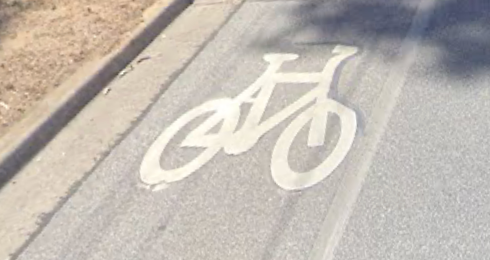
\includegraphics{f001_symbol.png}
\caption{Example bicycle lane marking.  Source: Google Street View, Oct 2019}
\label{fig:symbol}
\end{figure}

This marking is universal across all standard bicycle lanes in Australia, and can distinguish a bicycle lane from other parts of the road.  It may sometimes appear on a green surface, and occasionally it may be partially occluded due to limited space or wear and tear.  Similar markings exist in many other jurisdictions outside Australia.

In order to train a deep learning model to recognise bicycle lane markings in street scene images, it was necessary to first create a dataset of labelled images for training and validation.  This could then be used to apply a variety of pre-trained models from the ``TensorFlow 2 Model Garden'' to the problem, through a process of transfer learning.

\subsection{Gathering a labelled dataset of Google Street View images}

The official Australian design standards for bicycle lanes specify that bicycle lane markings should appear within 15m of each intersection \cite{standards}.  Therefore, intersections along known bicycle lane routes are the locations where example images are most likely to be found.

Campbell et al., 2019 \cite{CAMPBELL2019101350} successfully trained a deep learning model to recognise ``Stop'' and ``Give Way'' signs with 500 example images of each.  Therefore, an initial dataset of 500 bicycle lane marking example images was gathered, with an option to gather more images later, if necessary.

A Jupyter Notebook was created to allow an operator to efficiently review Google Street View images from intersections along known bicycle lane, and record which image files included the required examples.  These images could then be ``labelled'', to record a precise bounding box around each bicycle lane marking in a format suitable for the TensorFlow 2 framework.

\subsubsection{Identifying candidate intersections to sample}
\label{s:sample_candidates}

Two possible sources of information about ``known'' bicycle lane routes were considered for use in the sampling process:  The ``Principal Bicycle Dataset'', and XML extracts from the OpenStreetMap database.  These datasets are discussed in detail in section \ref{s:datasets}.  The ``Principal Bicycle Network'' dataset was chosen, partially because it is the incumbent official dataset for policy makers in the area, and partially due to its age.  Given that it appears to have been last updated several years ago, then there is a much lower risk of attempting to sample an intersection, only to find that the bicycle lane was constructed too recently to appear in the available Google Street View data.  However, the approach of using OpenStreetMap as a source of ``known'' bicycle lane routes would have the advantage that it generalises to other jurisdictions, and the process involved in using it ultimately proved to be less complex than the ``Principal Bicycle Network'' approach.  Tools were created to generate lists of candidate intersections to sample in Google Street View using \textit{both} approaches.  For instructions on how to operate the tools, please refer to appendix \ref{aj01} to \ref{aj03}.

Working from an XML extract of the OpenStreetMap database is the simplest approach.  Data can be downloaded for an individual country via \url{https://download.geofabik.de} and then sliced into a smaller area, if necessary, using the ``osmium'' command line tool from \url{https://osmcode.org/osmium-tool/}.  For more background on concepts in the OpenStreetMap data, please refer to Appendix \ref{a:osm_concepts}.  Briefly, an OpenStreetMap XML extract file contains ``ways'', which usually represent road segments, and ``nodes'', which represent strings of coordinates that make up the ``ways'' and thereby describe the shape of the ``way'' on a map.  A list of candidate intersections along ``known'' bicycle lane routes can be extracted from OpenStreetMap XML data, as follows:

\begin{itemize}
\item{Use the ``osmium'' tool to reduce an OpenStreetMap database file for a country down to the required area.  The tool can either reduce the map to a required bounding box, or it can be asked for data about an arbitrary shape, based on official geographic boundaries for a town or Local Government Area specified in a geojson file.}
\item{Load the OpenStreetMap XML data into memory.  Find all ``way'' objects that include a ``cycleway'' tag.}
\item{For each ``way'' with a ``cycleway'' tag, check every ``node'' in the ``way''.  If a node is any other ``way'' where the tags indicate that it is a road, and the ``way'' has a different name, then the ``node'' is an intersection.  Include the ``node'' ID and its coordinates in the list of candidate intersections to sample.}
\end{itemize}

Working from the ``Principal Bicycle Network'' dataset is more complicated, because although it describes the shape of each bicycle lane route in geojson format, it does not have any information about intersections.  The data must be matched to OpenStreetMap to list the intersections along each route.  Another significant limitation is that it does not always list the name of the road for each bicycle lane route, and it never lists the town or suburb.  This makes it more difficult to match the ``Principal Bicycle Network'' data to another source to locate the intersections.  To overcome these limitations, the following approach was taken:

\begin{itemize}
\item{Explode each ``Principal Bicycle Network'' dataset record into a list of coordinates.}
\item{For each coordinate, use a ``Nominatim'' server instance to determine the names of the road and its town or suburb, via a ``reverse-geocoding'' API call.}
\item{For each coordinate and its named road and town or suburb, use an OpenStreetMap XML extract of the area to identify ``ways'' with a matching name, and then look up all ways that intersect with it.  Use a bounding box around the original route coordinates from the ``Principal Bicycle Network'' dataset to exclude streets in the OpenStreetMap data that just happen to have the same name, in another town.  E.g. ``Main Street'' might occur in many towns across the state.}
\end{itemize}

A local instance of ``Nominatim'' was installed and used for this purpose, because the terms of use for public instances discourage bulk operations, and limit them to one per second.  The local instance was configured on a machine as per Appendix \ref{a:computer}, following the official instructions \cite{nominatim_install}.  The instance was loaded with data for Australia only, and used a solid-state drive for storage.

Once intersections were identified, it proved to be helpful to also calculate an approximate heading along the bicycle lane route at each intersection, to ensure that Google Street View images could be requested with the camera facing in a sensible direction.  The Python ``geographiclib'' library can calculate a heading from one point to the next.  Therefore, a heading was calculated from the previous ``node'' on the ``way'' to the intersection ``node'', and from intersection ``node'' to the next ``node'', and then the heading at the intersection was assumed to be the average of the two headings.


\subsubsection{Downloading sample Google Street View images for the dataset}
\label{s:sample}

Google provides an API for downloading Google Street View images of up to 640x640 pixels, at a cost of \$7.00 USD per 1,000 images.  Volume discounts are available, with a reduced cost of \$5.60 USD per 1,000 image for volumes from 100,001 to 500,000 images, and beyond that, further volume discounts can be negotiated with Google's sales team \cite{gsv_billing}.

The Python ``google\_streetview'' library was used to facilitate access to this Google Street View API from Python code.  In order to minimise costs, whenever an image was downloaded via the API, a copy of the image and its associated metadata was cached locally at a path that depended on the request parameters.  If a request was made for the same image at a later date, it would be retrieve from disk instead of issuing a further request to Google, to minimise costs.

The Google Street View API allows images to be requested for a location (latitude/longitude) with a desired heading, field-of-view angle, and camera angle relative to the ``horizon''.  A Jupyter Notebook was created to:

\begin{enumerate}
	\item{Randomly select a sample location and heading from a CSV of candidate intersections anywhere in the State of Victoria.}
	\item{Download four Google Street View images at 0, 90, 180, and 270 degrees relative to the desired heading, with a 90 degree field of view for each image, and the camera angled 20 degrees towards the ground to focus on any nearby road markings.}
	\item{Allow the operator to quickly record which of the four images they see a bicycle lane marking in (if any) to a CSV file listing images ready to be labelled and included in the dataset.}
	\item{Repeat.}
\end{enumerate}

It was found that the best location to look for a bicycle lane marking was not always right in the middle of an intersection, especially for large intersections.  Therefore, the option was added to allow the operator to ``browse'' a desired number of metres before or after the intersection, along the route heading, to find a good image.  If a bicycle lane marking appeared at the intersection, typically it could be found within 20-30m, except for major intersections where bicycle lanes may be terminated early by turning lanes.

Generally, an image was accepted for inclusion in the dataset if the bicycle lane marking was clear and unambiguous without needing to take cues from the overall scene context.  If the symbol was so far away that it looked like a white blob on the road, and it could only be understood to be a bicycle lane marking based on its position relative to lane markings, then the image was not included, though the operator had the option of moving the camera closer for a better image.

The Jupyter Notebook allowed multiple candidate intersections to be assessed per minute, and an initial set of 500 images was collected over the course of approximately 4 hours.

Please see Appendix \ref{aj04} for detailed instructions on how to use the supplied Jupyter Notebook to download Google Street View images for sample candidate intersections, and flag matching images in an output CSV file for inclusion in the labelled dataset.


\subsubsection{Labelling the dataset}
\label{s:label}

Once a suitable number of Google Street View images containing bicycle lane markings were collected, they were copied to a folder and then labelled using the open-source tool ``labelImg'' \cite{labelImg}.  Please refer to appendix \ref{aj05} for more information on how to perform the labelling process.  The output of the process was one XML file per image, in a format that could be understood by TensorFlow 2 training tools and scripts.

\subsection{Training and evaluating candidate models from the TensorFlow 2 Model Garden}

Training and evaluation of candidate models was conducted on local infrastructure, as described in Appendix \ref{a:computer}.  This task could also be performed on cloud-based infrastructure such as Google Collab, if required.  For general directions on how to set up a local computer to enable TensorFlow machine learning that takes advantage of GPU acceleration, please search online for the latest tutorials and guides, as this may be subject to change over time.

The dataset that was collected in section \ref{s:sample} and labelled in section \ref{s:label} was randomly split into ``training'' and ``testing'' datasets according to an 80:20 ratio.

A Jupyter Notebook was used to set up the experiment, by transforming the labelled image datasets into TensorFlow records, downloading and configuring a pre-trained model from the TensorFlow 2 Model Garden, and creating scripts to train and evaluate the model.

The performance of each model usually be influenced by three significant factors:

\begin{itemize}
\item{The size of the dataset available for training and validation.}
\item{The number of epochs spent training, where an ``epoch'' is a training iteration where a complete pass is made over the training dataset.}
\item{The threshold confidence score, from 0\% to 100\%, at which the model assumes that a bicycle lane marking has been detected.}
\end{itemize}

The initial size of the dataset was set based on previous experience in other papers such as Campbell et al., 2019 \cite{CAMPBELL2019101350}, with the option to extend it later if necessary.  In practice, it was found that the initial size was sufficient to obtain good results for detections from Google Street View images, and no further training images were required.

During the training process, the TensorFlow 2 training script reports ``loss'' performance metrics every 100 epochs.  The performance reported by the training script gradually improved as more training was conducted over the dataset.  Every 2000 epochs, training was paused, and the TensorFlow 2 evaluation script was run to test the performance of the model against the independent testing dataset that had been withheld from the training process.  When training reached the point that further epochs did not significantly improve performance in either the training or the evaluation, training was halted.

As part of the evaluation process, image files were written to disk, containing the original image plus an overlay where the bounding boxes and confidence score of any detections were drawn.  These were examined to determine how many false positives and false negatives there were, and the confidence scores when the model returned any false result.  The threshold confidence score was tuned in response to these findings, to find as many true positives as possible without significant numbers of false positives that might cause bicycle lane routes to be ``detected'' where they do not really exist.

The boundary boxes of detections were also checked to ensure that the results were sensible.

Multiple pre-trained models from the TensorFlow 2 Model Garden were trialled, with selections guided by their advertised ``Speed'' and ``COCO mAP'' (mean Average Precision) metrics.  The process of building a map of bicycle lanes for an area can be considered a ``batch'' process, with no fixed time constraints, therefore mean Average Precision was prioritized over speed.

The TensorFlow 2 Model Garden provided an efficient way to test multiple models via a single framework.  However, there are popular object detection models, such as the ``YOLO'' series of models, that are not supported by it.  For the purposes of this research, it was not considered necessary to perform an exhaustive search of all possible models across multiple frameworks.  However a different model (e.g. YOLOv3) or a different framework (e.g. PyTorch) could be substituted if required.

Please refer to Appendix \ref{aj06} for detailed instructions on how to reproduce the training process.

% ~~~~~~~~~~~~~~~~~~~~~~~~~~
\section{RQ2: Building a map of bicycle lane routes from Google Street View images in an area}
\label{s:rq2}

In section \ref{s:rq1}, a model was trained to detect bicycle lane markings in one street view image at a time.  To generate a map or dataset of bicycle lanes in an area, the first step is to determine a list of locations for which Google Street View images should be downloaded and processed by the model.  A batch process can then used to process each image and record whether or not a bicycle lane marking was found.  Finally, the list of sample locations where there was a ``hit'' must be correlated to geospatial data about the road network to infer routes, draw them on a map, and compare them to other sources.


\subsection{Sampling strategy for Google Street View images}
\label{s:rq2a}

In section \ref{s:sample}, it was noted that Google currently advertises a minimum cost of \$7.00 USD per 1,000 Google Street View images, and that the most likely place to find a bicycle lane marker is in the area immediately surrounding an intersection.  During the sampling process, it was found that the Google Street View API would only return distinct images every 10 metres.  Two sampling strategies were considered:
\begin{itemize}
\item{Generating a list of sample points every 10 metres along every street in the area.}
\item{Generating a list of sample points within a configurable distance of each intersection in the area, at 10 metre intervals.	}
\end{itemize}

Depending on the density of intersections in an area, limiting the samples to the immediate area around intersections could result in a significant cost reduction.  The ``intersection'' strategy was chosen, with the option to switch to a strategy of sampling every 10 metres if the results showed that too many bicycle lanes were being missed in situations where they might have been detected with more samples.

An OpenStreetMap XML extract file for the area was loaded into memory and used to iterate over all streets and intersections in the area, resulting in a CSV batch file of sample locations to be downloaded from Google Street View and processed by the model.  The size of the batch file was inspected to assess potential cost before proceeding with the download of images from Google Street View.

When loading and interpreting the OpenStreetMap XML extracts, it was important to understand that while a ``way'' object in the data typically represents a road segment, it may instead represent the boundary of a reserve, a natural feature such as a coastline or creek, or a walking trail.  A ``way'' is used to represent any line that is drawn on the map, in general.  To avoid unnecessary requests to the Google Street View API for off-street locations, it was necessary to inspect the ``tags'' associated with each ``way'' to isolate actual road segments.

Another important consideration was how to handle roads that form the boundary of the area being surveyed.  If the ``osmium'' tool is used to create an OpenStreetMap XML extract for a precise area according to a shape in a geojson file describing the official boundary, then the resulting extract may inadvertently exclude intersections where the intersecting road exists entirely outside the boundary.  This problem was addressed by allowing the operator to load a second OpenStreetMap XML extract file to cover bounding box with a 200 metre margin around the area being surveyed.  Streets in the margin would not be considered in the survey for possible bicycle lane routes, but they provided supplementary used only to identify intersections and ensure that none were missed.

Once the sampling process has been run, the output is a CSV with the coordinates of each point to be downloaded from Google Street View and examined by the detection model.  The CSV file includes additional columns to record the OpenStreetMap ``way'' ID and ``node'' ID associated with each point, so that any results can be linked back to the map.  Other fields such as the street name were also included for traceability.

Please see appendix \ref{aj09} and \ref{aj10} for detailed instructions on how to operate the tools that were used to generate a list of sample locations in a survey area.


\subsection{Batch processing of Google Street View images}
\label{s:rq2b}

Given a CSV file listing sample locations for the survey area, a batch process works through the list, downloading any Google Street View images that have not already been cached locally.  Then, the selected detection model is called to process each image in turn.  If one or more bicycle lane markings are detected in an image, a copy of the image is saved to a folder of ``hits'', with the bounding box and confidence score included in the image as an overlay, to show where the detection was found.  A record is also inserted into a CSV file of detection locations.  If no bicycle lane marking is found in the image, a copy is instead placed in a separate ``miss'' folder.  Partitioning the result images into separate  ``hits'' and ``misses'' folders allows the operator to quickly browse the images to check for any false positives or false negatives.


\begin{figure}[h!]
\centering
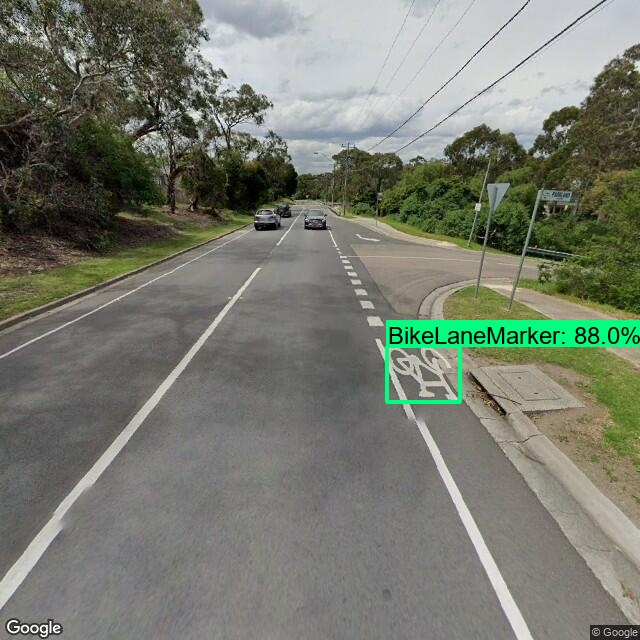
\includegraphics[width=0.5\linewidth]{f004_gsv_detection_example.jpg}
\caption{Example bicycle lane marking with detection overlay.  Source: Google Street View, Oct 2019}
\label{fig:004}
\end{figure}

Please see appendix \ref{aj10} for detailed instructions on how to operate the tool that was used to download and cache Google Street View images for a list of sample locations, then process them with the model.


\subsection{Converting detection points into bicycle lane routes on a map}
\label{s:rq2c}

The result of the batch process in section \ref{s:rq2b} is a list of locations where a bicycle lane marking was found, linked to the OpenStreetMap ``way'' IDs and ``node'' IDs that they were sampled from.  The next step is to convert these detection points into contiguous routes that can be drawn as lines on a map.

Google Street View image samples were taken 0, 90, 180, and 270 degrees from the assumed heading at each point, to provide 360 degree coverage.  This allows detection of bicycle lane markings not just in the the forward and rear views, but also close alongside the camera vehicle, to improve the chances that an image will be found where the marking is clearly visible.  The detection model has been trained to detect markings in any orientation, and many of the samples will be taken at intersections.  Therefore, when drawing routes, proper consideration must be made about whether a detection belongs to the route being inspected, or an intersecting street.

Routes were inferred from the individual detection points based on the assumption that if markings were detected at two or more consecutive intersections along a named road, there is a bicycle lane along that segment.  A configuration option was provided to allow for one or more intersections with ``missing'' detections before assuming that the bicycle lane route has been interrupted.

A continuous road may be divided up into multiple ``way'' segments in the OpenStreetMap data if any of its characteristics change from one segment to the next, such as a change of speed limit.  Before inferring bicycle lane routes along a road from the detection points, it was necessary to link adjacent ``way'' segments from a single named road back up into a single chain.  Otherwise, the option to allow for intersections with ``missing'' detections would not always work as intended.

Each inferred route was written to a geojson file as a ``LineString Feature'', following the coordinates of all ``nodes'' in the original OpenStreetMap ``way'', from start to finish.


\subsection{Comparing results to other data sources}

Once a geojson file has been produced to describe the detected bicycle lane routes, it can be drawn on a map in a Jupyter Notebook using the Python ``ipyleaflet'' library.

The total length of all routes in a geojson file can be calculated by using the Python ``geographiclib'' library to measure the distance between each pair of points along the route.

The OpenStreetMap XML extract for the survey area can be used to generate an equivalent geojson file of bicycle lane routes according to OpenStreetMap.  The data is filtered down to ``ways'' that are roads and have a ``cycleway'' tag.  Then a ``LineString Feature'' is written to an output geojson for each cycleway.

The detected routes geojson file and the OpenStreetMap-derived geojson file can be drawn on maps side-by-side for visual comparison, and the differences can be measured at a high level by comparing the total length of the routes in each file.

To drill down further into the detail of the differences, multiple geojson files were created:

\begin{enumerate}
\item{A geojson file with all bicycle lanes from the detection model}
\item{A geojson file where a bicycle lane was detected but was not recorded in OpenStreetMap}
\item{A geojson file where a bicycle lane was recorded in OpenStreetMap but not detected}
\item{A geojson file where both the detection model and OpenStreetMap agree that there is a bicycle lane}	
\end{enumerate}

Items 2-4 can be drawn as layers on a single map, each with their own color, to highlight where the bicycle lanes are, and where the sources agree and disagree.  By measuring the distances in each geojson file, we can quantify how much agreement there is between the two sources, and how many metres worth of bicycle lane routes are in dispute.

Where there is a disagreement between the output of the detection model and what has been recorded in OpenStreetMap, the original images or footage can be reviewed to establish the truth, and whether the detection model was producing reasonable results for its input.

The ``Principal Bicycle Network dataset'' is available in a geojson format.  A quick visual comparison is therefore possible, by drawing it on a map side-by-side with the geojson file of detected bicycle lane routes.  To quantify the differences in more detail:

\begin{enumerate}
\item{For each point in the ``Principal Bicycle Network'' dataset geojson file, find the closest point in the OpenStreetMap XML extract and its ``node'' ID.  Exclude any points outside the bounding box of the survey area.}
\item{Use the coordinates of the matching ``node'' from the OpenStreetMap data, instead of the original coordinates from the ``Principal Bicycle Network'' dataset, to ensure that the sources are ``aligned'' on a common understanding  of where the road network is, and eliminate tiny differences.}
\item{Produce four output geojson files to compare the ``aligned'' ``Principal Bicycle Network'' data to the detected bicycle lanes, following the same basic process that was used for the OpenStreetMap comparison.}
\end{enumerate}


% ~~~~~~~~~~~~~~~~~~~~~~~~~~
\section{RQ3: Applying the process to dash camera footage}
\label{s:rq3}

The use of Google Street View images for detection of bicycle lanes has both advantages and disadvantages to consider.  Google Street View image data is readily available for a wide area across many jurisdictions internationally, and it can be collected without a physical presence on location.  However, usage comes at a cost, which may be a significant factor if mapping is required across a large area.  The image resolution is limited to 640x640 per image, though perhaps this can be worked around by requesting many more images per location, each with a tighter field of view, at additional cost.  It appears that distinct images are only available every 10 metres.  The images may be several years out of date.  The position of the camera cannot be controlled, and it might miss service roads or the other side of a divided road.  With only one image available for each location, a bicycle lane marking might be obscured due to bad luck with other traffic.

A local authority might prefer to gather their own footage, to address these shortcomings.  For the third research question, we explore whether bicycle lanes can be detecded using dash camera footage instead, perhaps captured from vehicles that must regularly traverse the roads in the area to provide other services, such as waste disposal or deliveries.


\subsection{Choice of dash camera hardware}
\label{s:rq3a}

For these experiments, the ``Navman MiVue 1100 Sensor XL DC Dual Dash Cam'' was self-installed inside a passenger sedan in the manufacturer's recommended location behind the rear-view mirror, at a cost of \$529 AUD.  This model was selected because for each one minute of footage recorded in an MP4 video file, it also records an NMEA file with latitude, longitude, heading, and altitude at one second intervals.  The NMEA metadata allows each frame in the footage to be linked to a location, by correlating the frame number to nearest NMEA measurements, and extrapolating readings across the 1 second interval as required.

Video footage was recorded at 60 frames per second, at 1920x1080 resolution, a significant improvement on the 640x640 resolution of Google Street View images, and the 10 metre intervals.  Only images from the front-facing camera were used.

The camera features a ``wide angle'' lens to capture a good view of the road and its general surroundings, however optical specifications such as focal length were not available from the manufacturer's website.


\subsection{Gathering and processing dash camera footage}
\label{s:rq3b}

On the 3rd of October, 2021, Melbourne set the record for the longest ``COVID lockdown'' in the world \cite{lockdown_record}.  Severe restrictions were placed on residents being more than 5km from home, gradually easing to 10km and then 15km for a period of many months during the course of the research\cite{lockdown_5km}.  Permitted reasons to leave home were restricted.  Therefore it was only possible to experiment with dash camera footage from a confined area.

Approximately 100 minutes of footage was gathered by driving within a local area around the outer metropolitan suburbs of Mount Eliza, Frankston, Langwarrin and Baxter in Melbourne, Victoria, Australia.  Not every road in the area was covered.  Roads were selected for inclusion in the footage to include all known bicycle lanes in the area, based on local knowledge and a review of the OpenStreetMap data.  A variety of other roads were included, to cover roads with and without a paved shoulder, major divided roads and small local roads, and a mix of residential and commercial areas.

The dash camera video footage and corresponding NMEA files were transferred to a computer for processing via MicroSD card.  Then a batch process was set up in Jupyter Notebook to process each pair of files in a directory.

For each pair of files, the NMEA file was loaded into memory, then the video file was split into a series of images via the ``OpenCV'' library.  Reviewing the footage, it was decided that it was only necessary to process every 12th frame in order to get a clear view of every bicycle lane marking, effectively reducing the footage from 60 frames per second to 5 frames per second.  The latitude, longitude, altitude, and heading for each frame was calculated or extrapolated from the NMEA records.  Each frame was recorded to disk as a .png file, with a filename consisting of the original video filename, and a four-digit frame number.  Browsing these files in alphabetical order preserved their original chronological sequence.  For each frame, an entry was added to an output ``batch'' CSV file to record the path to the image file to be processed, and its associated location metadata.

The batch CSV file was processed by the detection model to yield another CSV file with detection results, as per the Google Street View process described in section \ref{s:rq2}.  For images where at least one bicycle lane marking was detected, a copy of the image with a green bounding box was written to a ``hits'' directory for manual inspection.  For images where a bicycle lane marking was not detected, a copy was written to the ``miss'' directory.  Images in the ``hits'' and ``miss'' folders could be quickly inspected manually.


\subsection{Training the bicycle lane detection model}
\label{rq3c}

The dash camera footage was initially processed using the original model that was trained exclusively on Google Street View images in section \ref{s:rq1}, without any retraining based on dash camera images.  The original model was able to detect every bicycle lane marking in the test footage, however further training and refinement was required to address some performance issues:

\begin{itemize}
\item{Although the Google Street View-trained model was able to detect every marking during initial trials, it typically only did so when the marking was very close to the camera vehicle.  Further training was apparently needed on footage from the dash camera in order to allow it to detect markings that were further away, but still close enough to be clearly visible.}
\item{There were also issues with false positives that had not been apparent when using the Google Street View model on Google Street View images.  The model would sometimes yield false positives in the following situations:

	\begin{itemize}
	\item{Short white dashes painted at intersections to advise drivers to ``give way''}
	\item{White arrows drawn on the road surface, such as turning lane arrows}
	\item{Diagonal white stripes that were drawn on the road to represent traffic islands}
	\item{Large white writing on the road, such as ``KEEP CLEAR''}
	\item{Pale road defects and anomalies}
	\item{Reflections from the bonnet of the camera vehicle}
	\item{Random objects or clouds well outside the boundary of the road}
	\end{itemize}
}
\end{itemize}

See figure \ref{fig:false_positives} for examples.

\begin{figure}[h]
\centering
\begin{subfigure}{0.3\textwidth}
	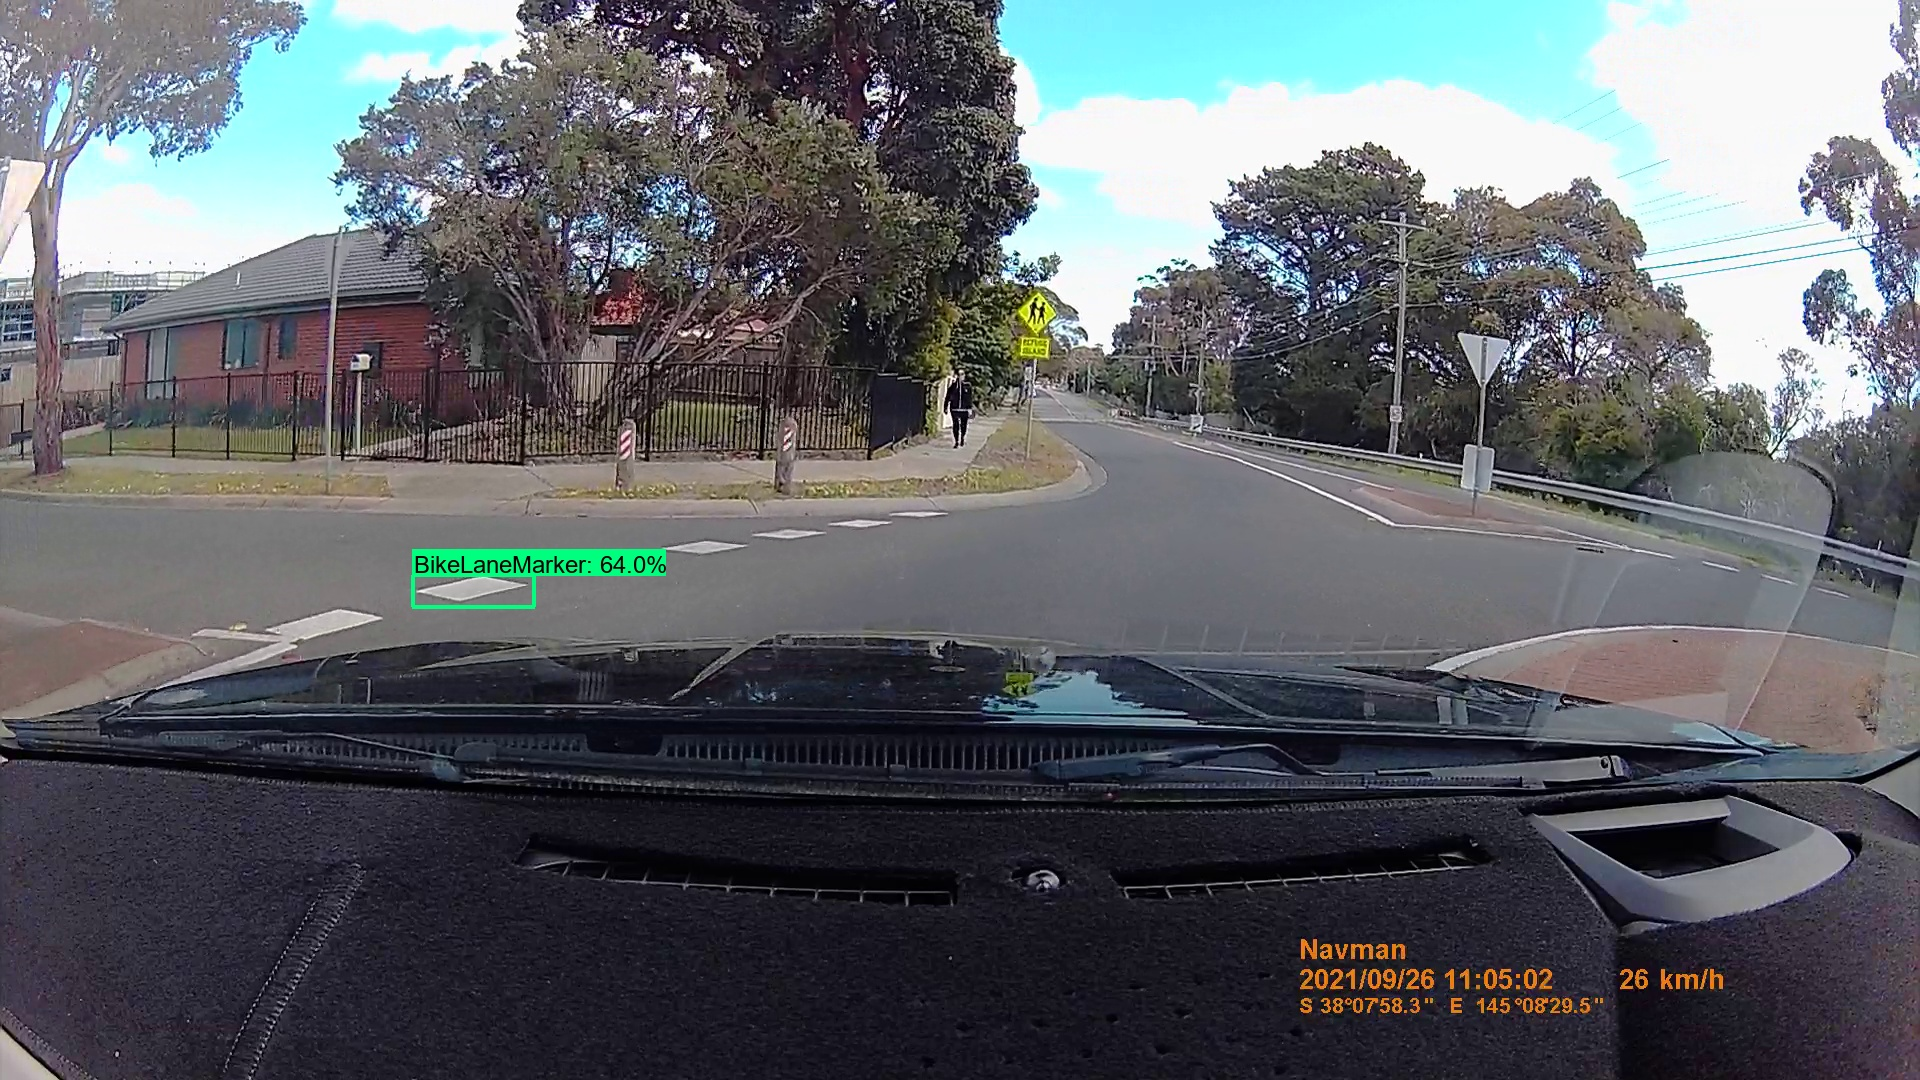
\includegraphics[width=\textwidth]{f005_false_positive_give_way.jpg}
	\caption{``Give Way'' stripes}
\end{subfigure}
\hfill
\begin{subfigure}{0.3\textwidth}
	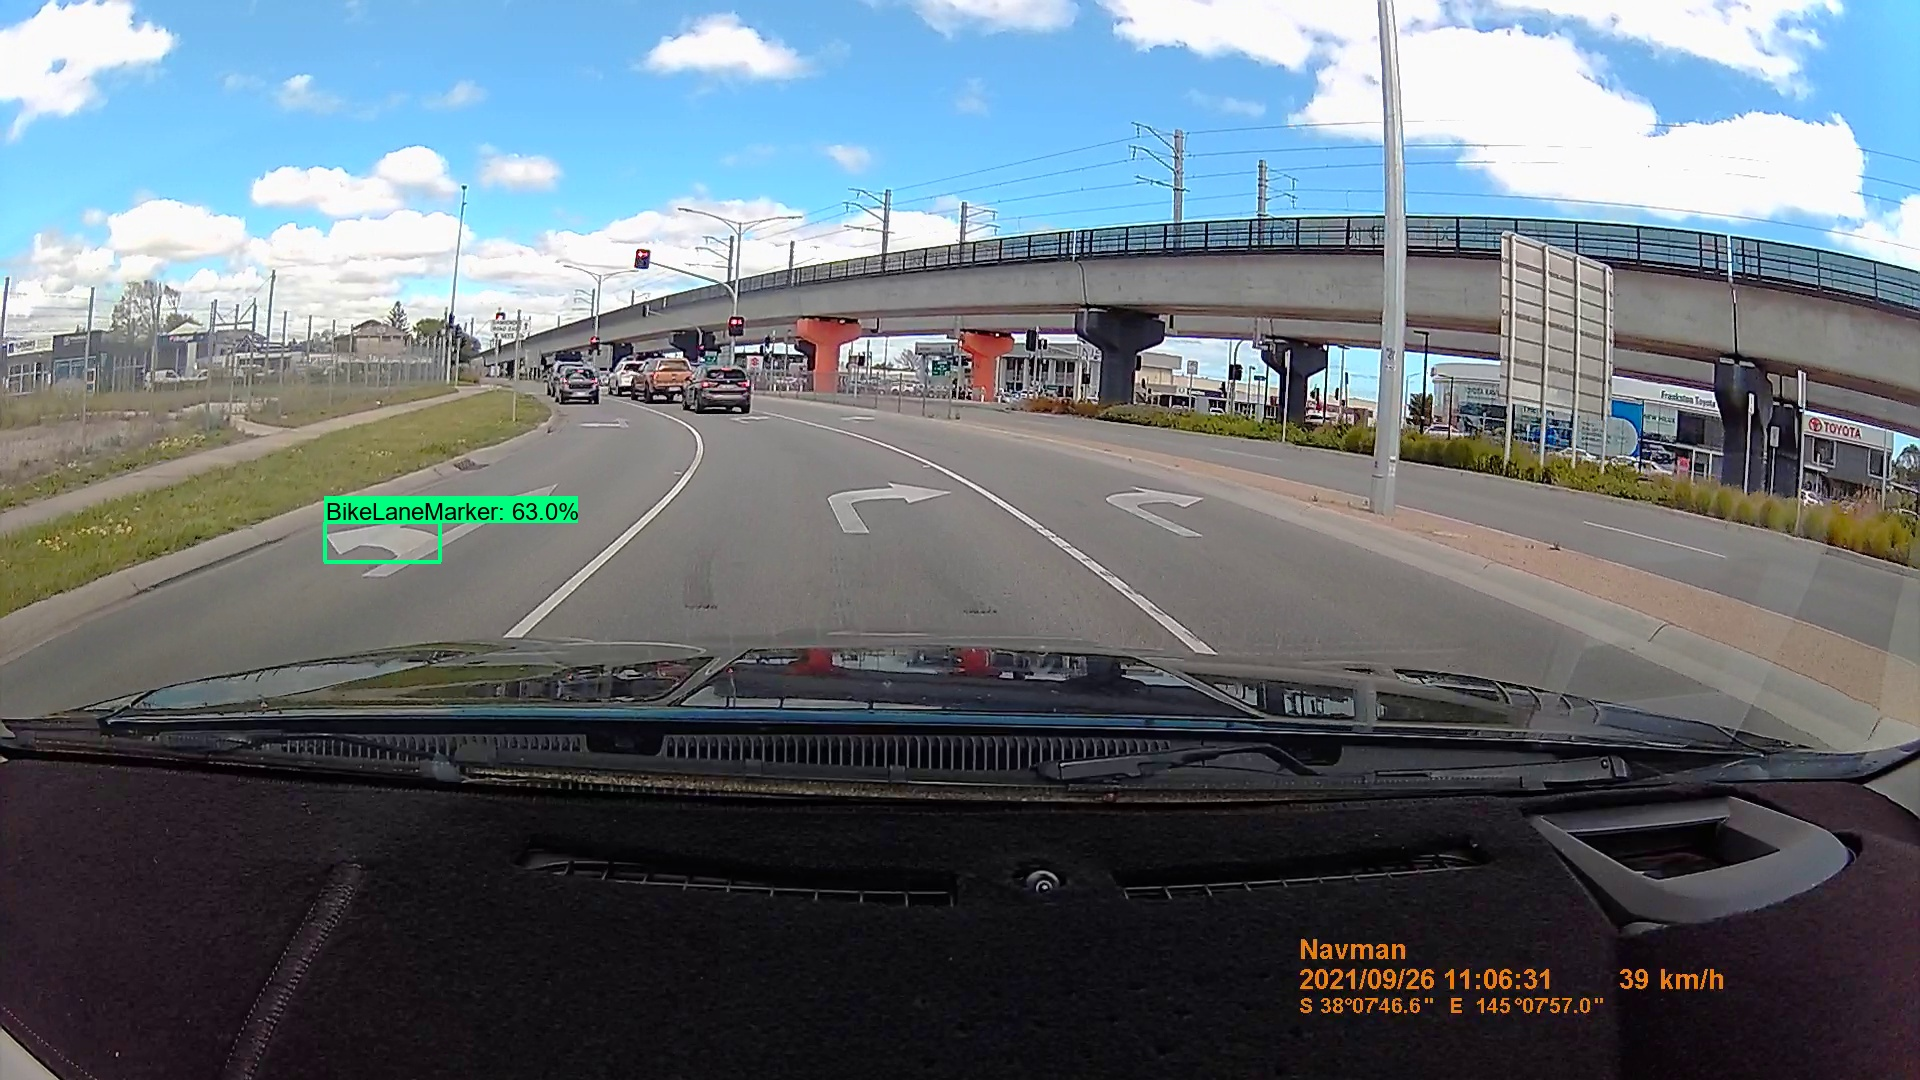
\includegraphics[width=\textwidth]{f005_false_positive_arrow.jpg}
	\caption{Turning arrow}
\end{subfigure}
\hfill
\begin{subfigure}{0.3\textwidth}
	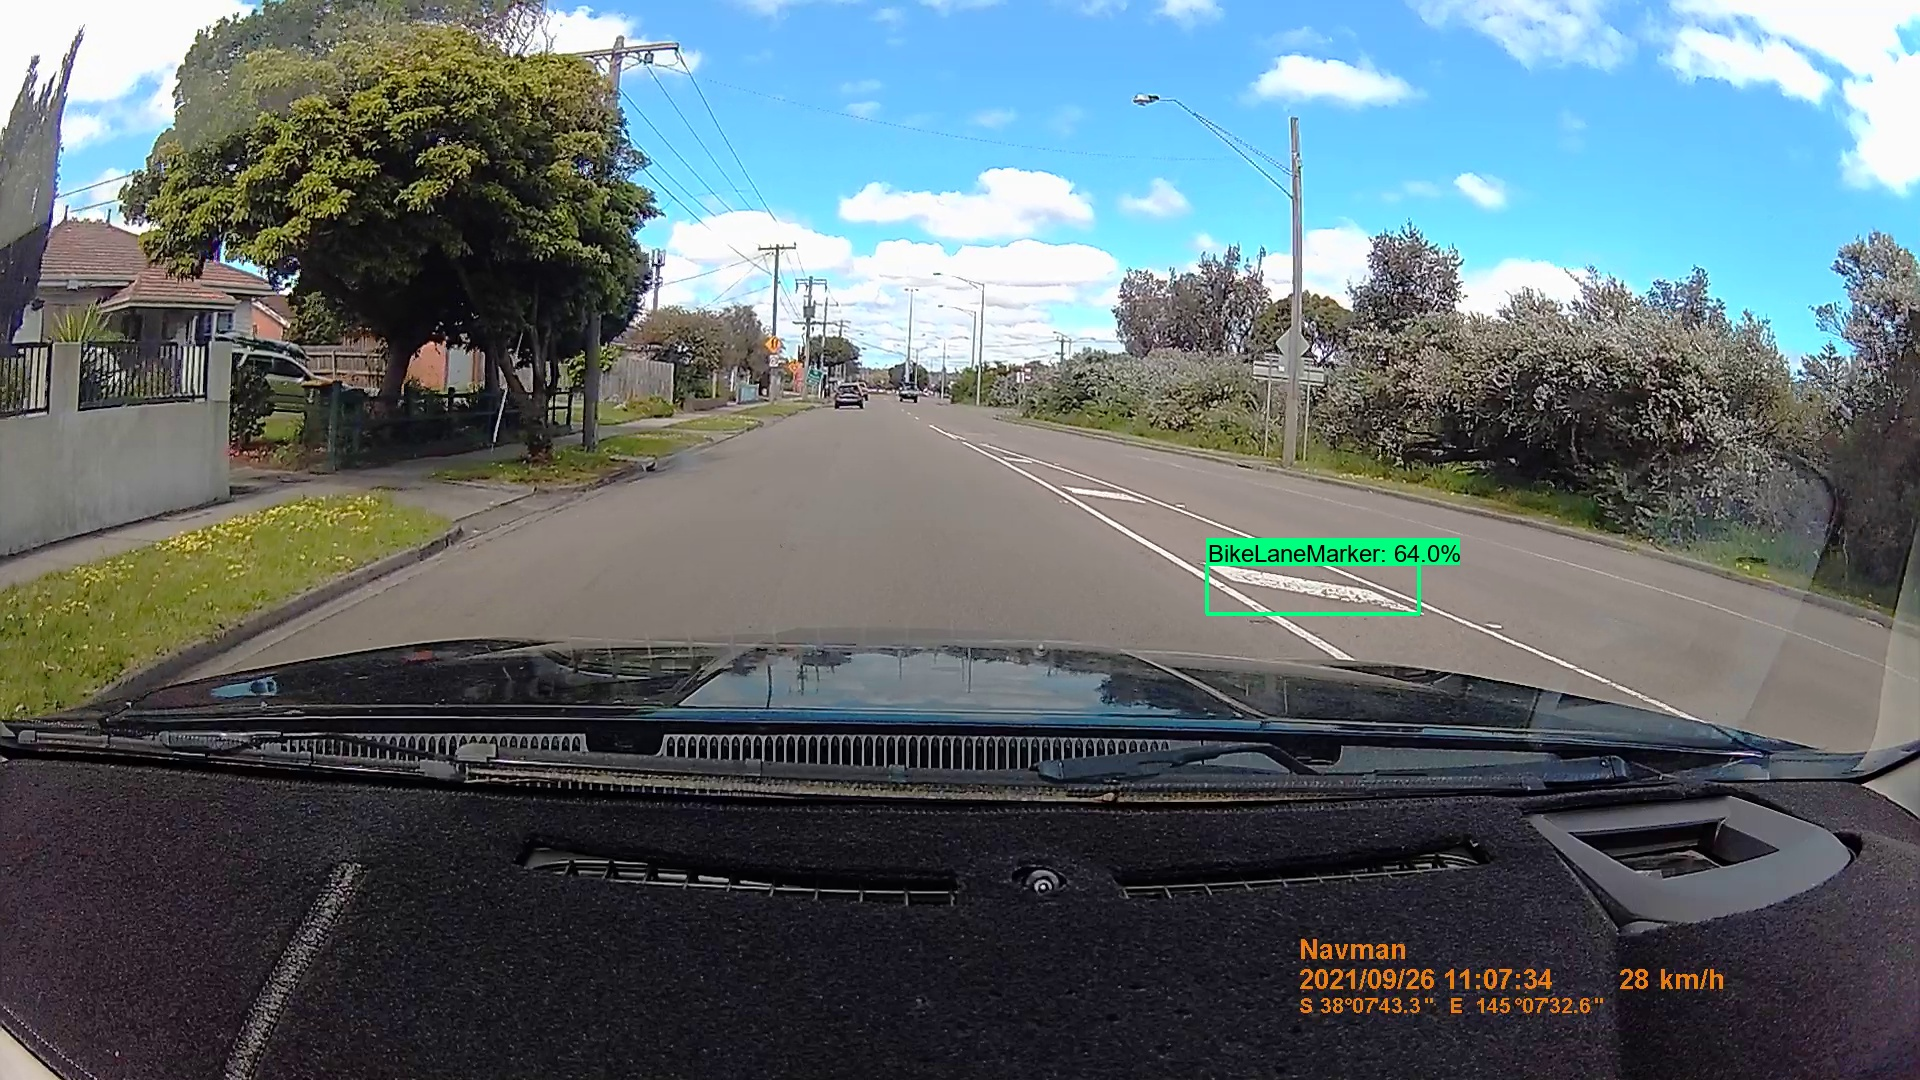
\includegraphics[width=\textwidth]{f005_false_positive_island.jpg}
	\caption{Traffic island}
\end{subfigure}
\hfill
\begin{subfigure}{0.3\textwidth}
	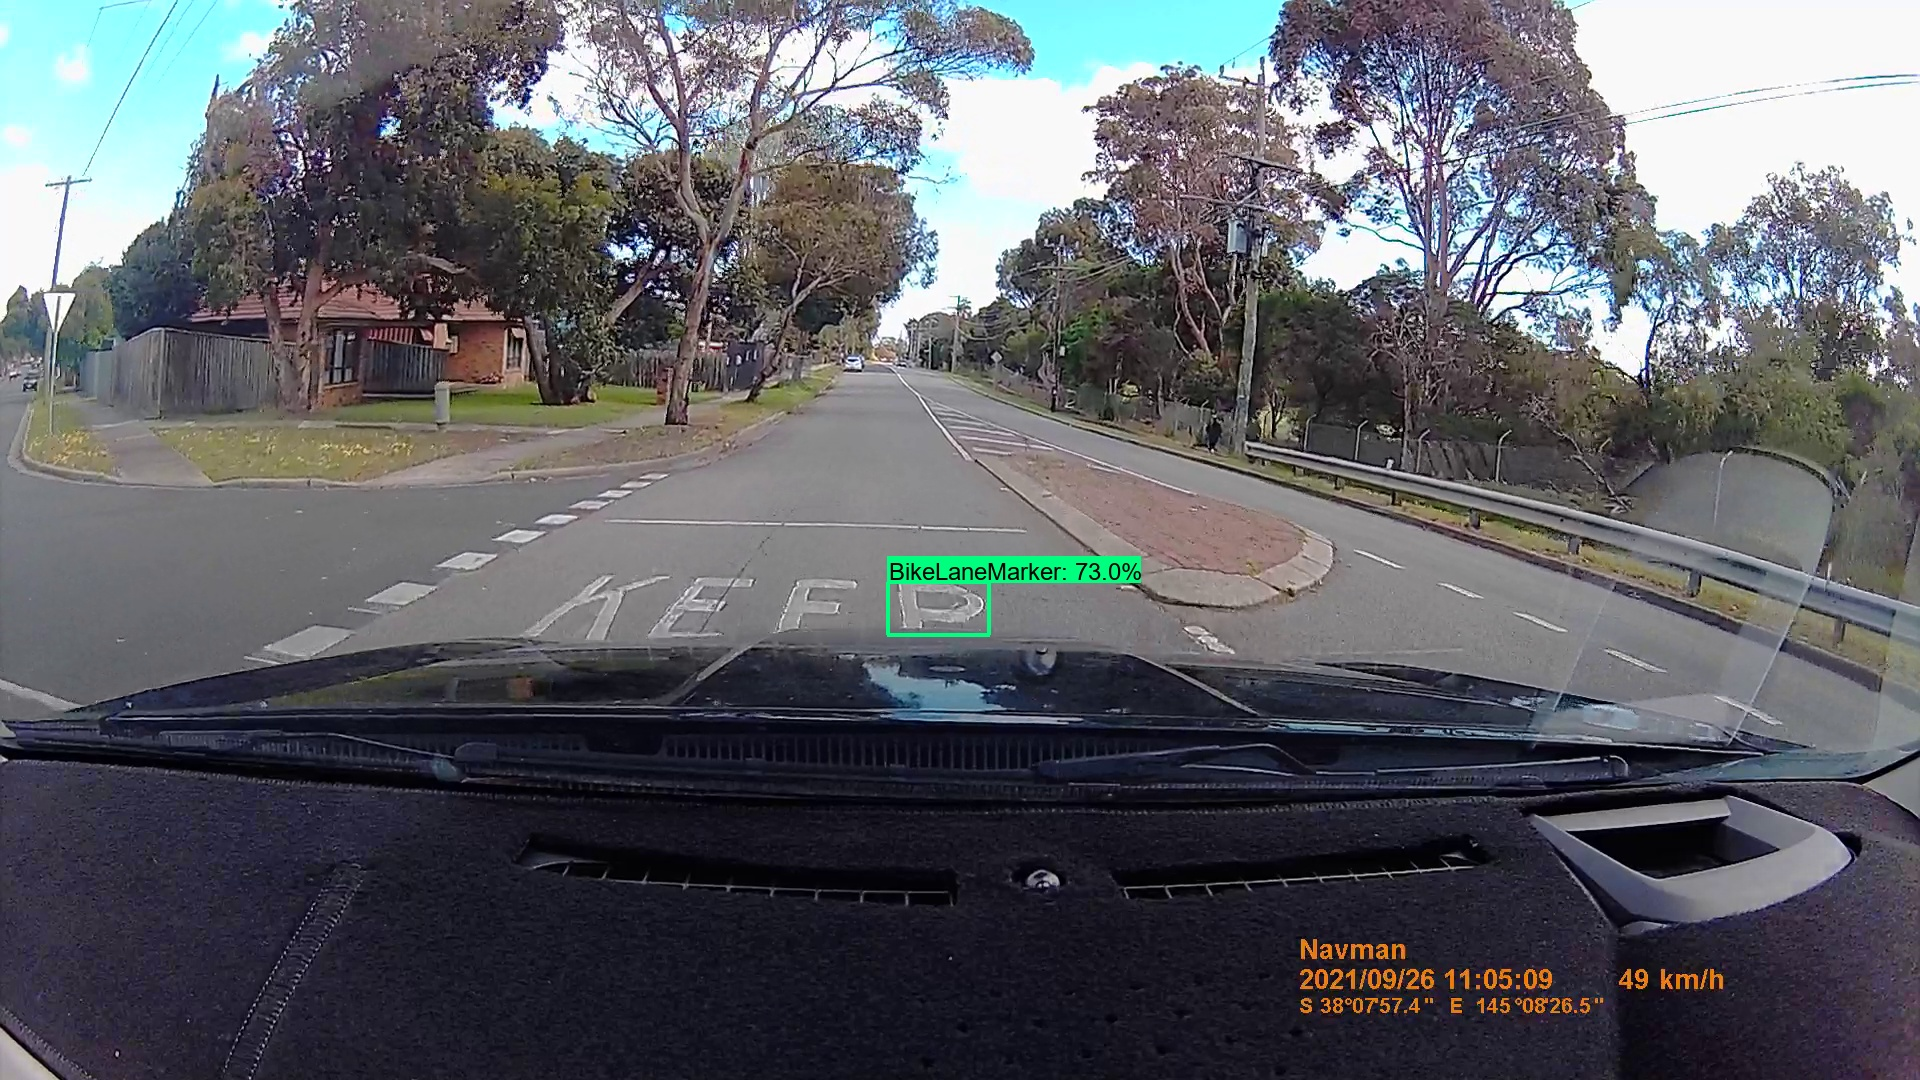
\includegraphics[width=\textwidth]{f005_false_positive_writing.jpg}
	\caption{``Keep Clear'' writing}
\end{subfigure}
\hfill
\begin{subfigure}{0.3\textwidth}
	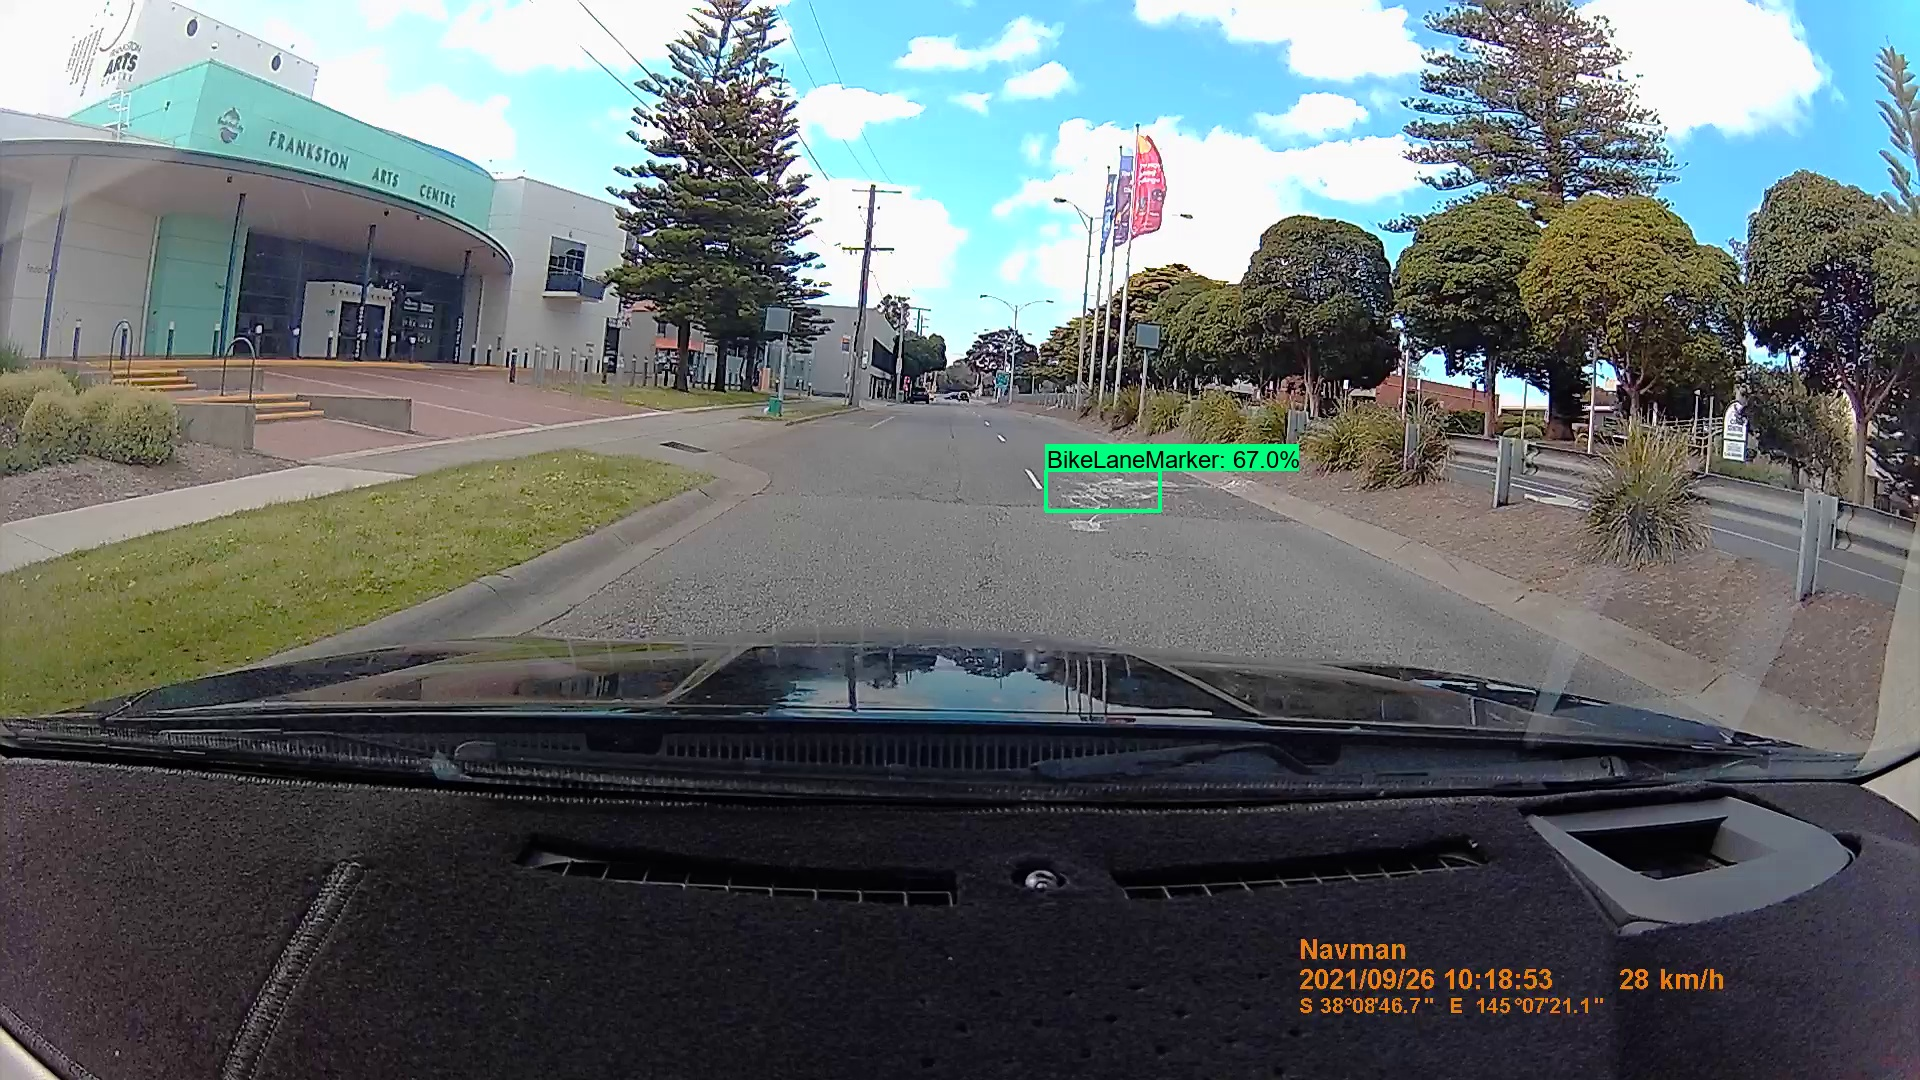
\includegraphics[width=\textwidth]{f005_false_positive_defect1.jpg}
	\caption{Road surface anomaly}
\end{subfigure}
\hfill
\begin{subfigure}{0.3\textwidth}
	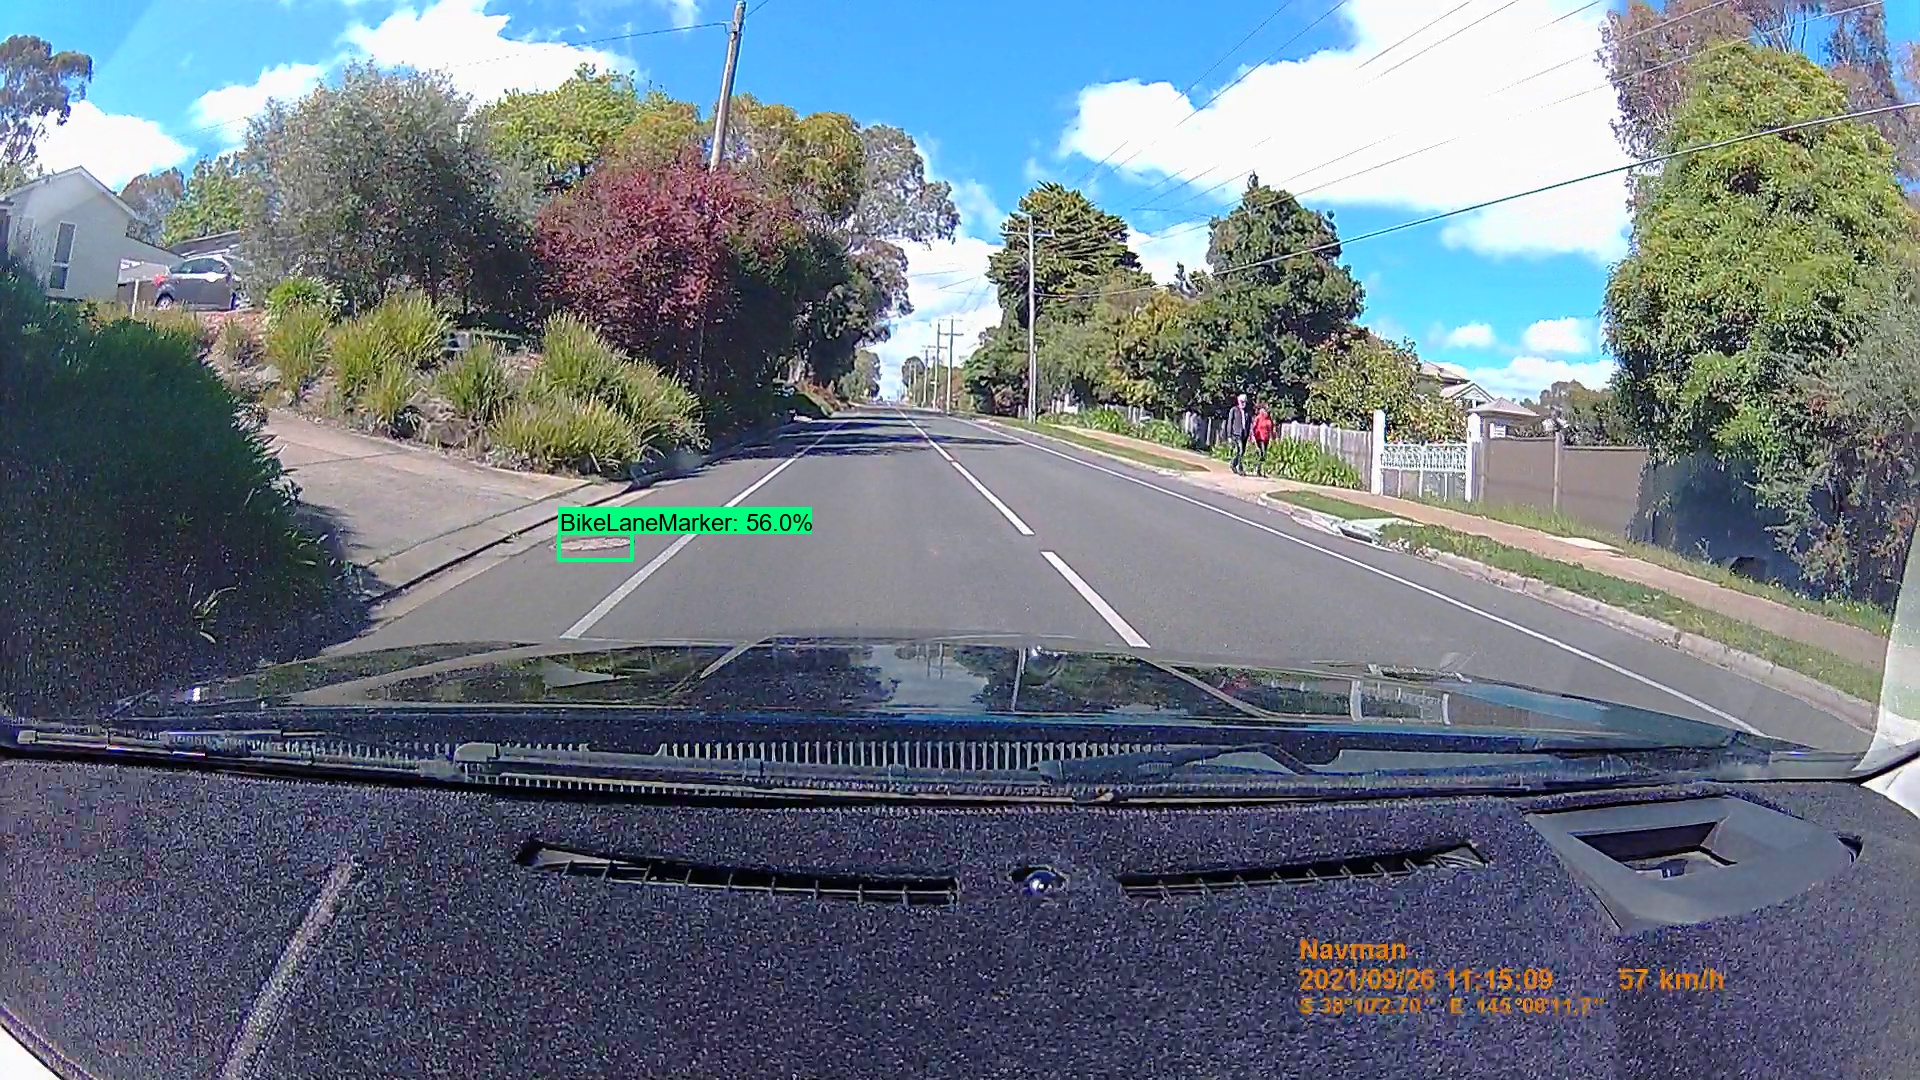
\includegraphics[width=\textwidth]{f005_false_positive_service_hatch.jpg}
	\caption{Road surface anomaly}
\end{subfigure}
\hfill
\begin{subfigure}{0.3\textwidth}
	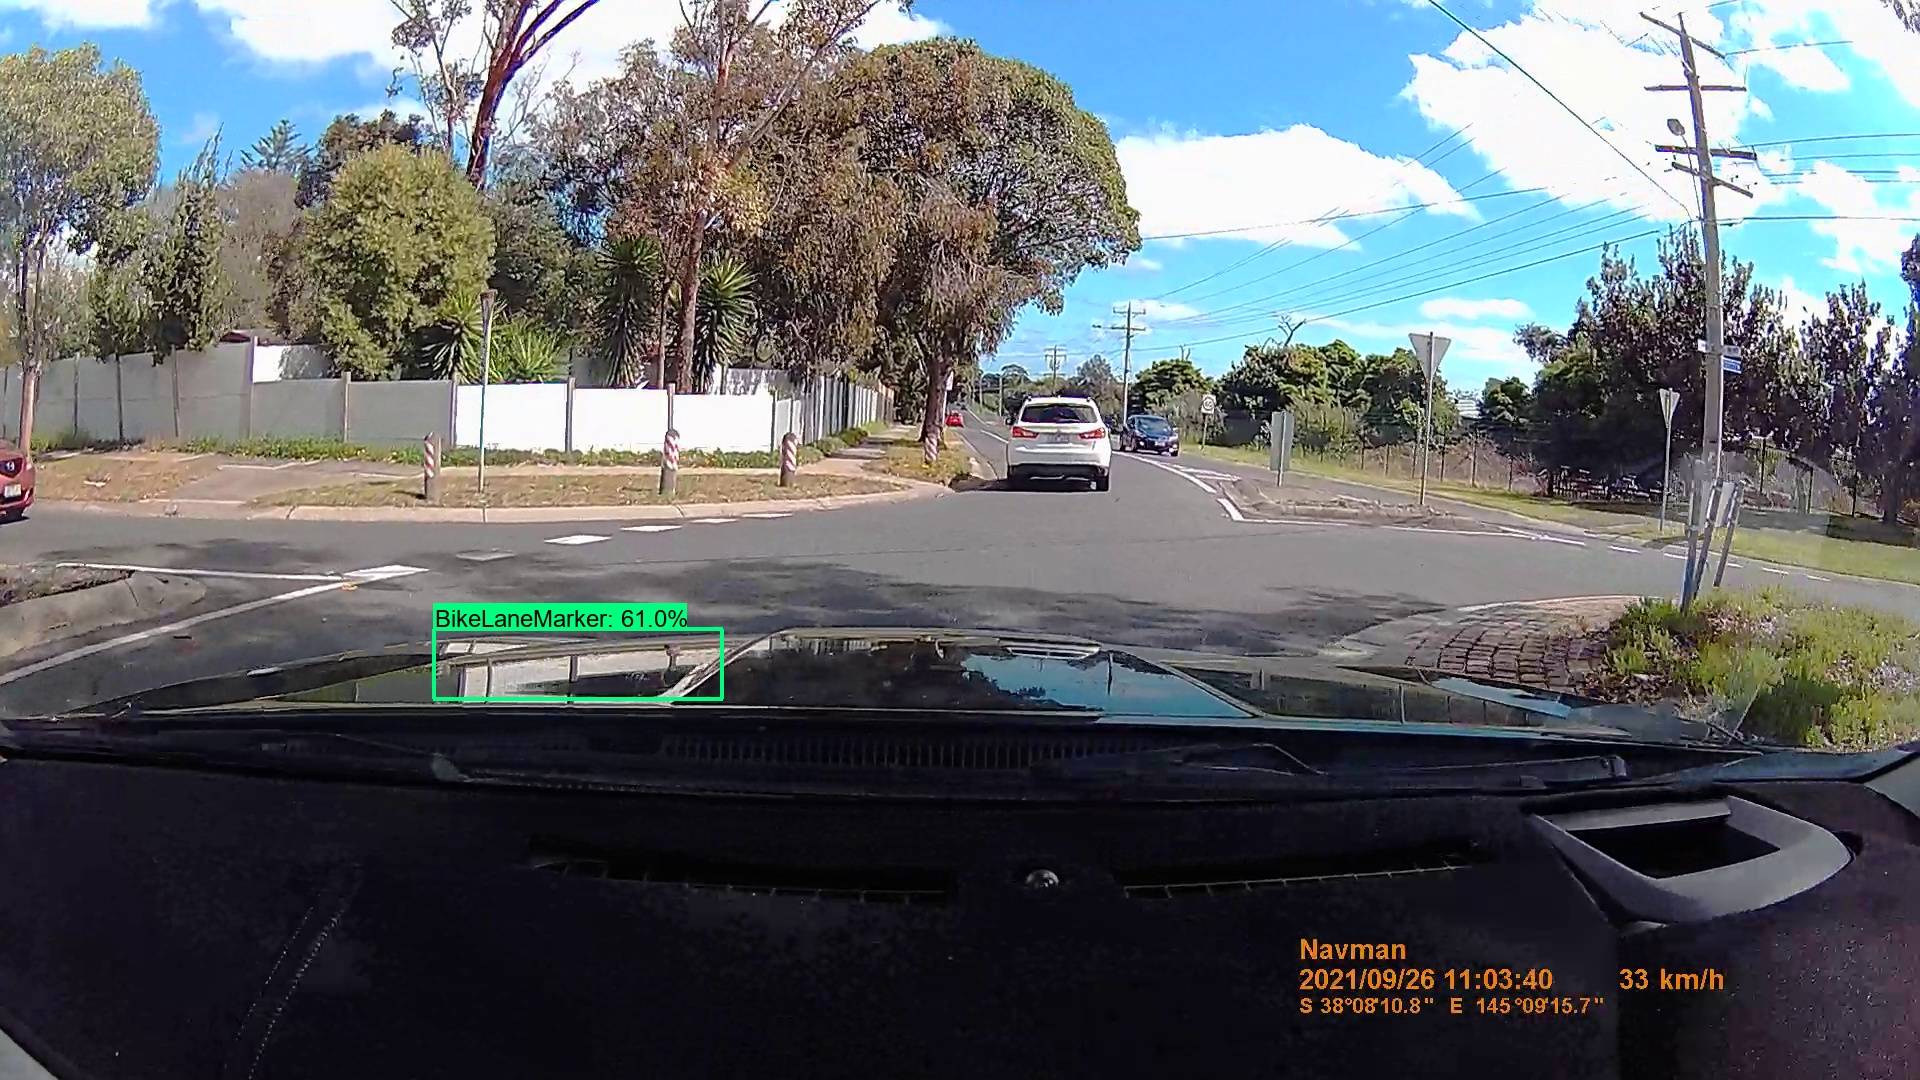
\includegraphics[width=\textwidth]{f005_false_positive_reflection.jpg}
	\caption{Bonnet reflection}
\end{subfigure}
%\hfill
\begin{subfigure}{0.3\textwidth}
	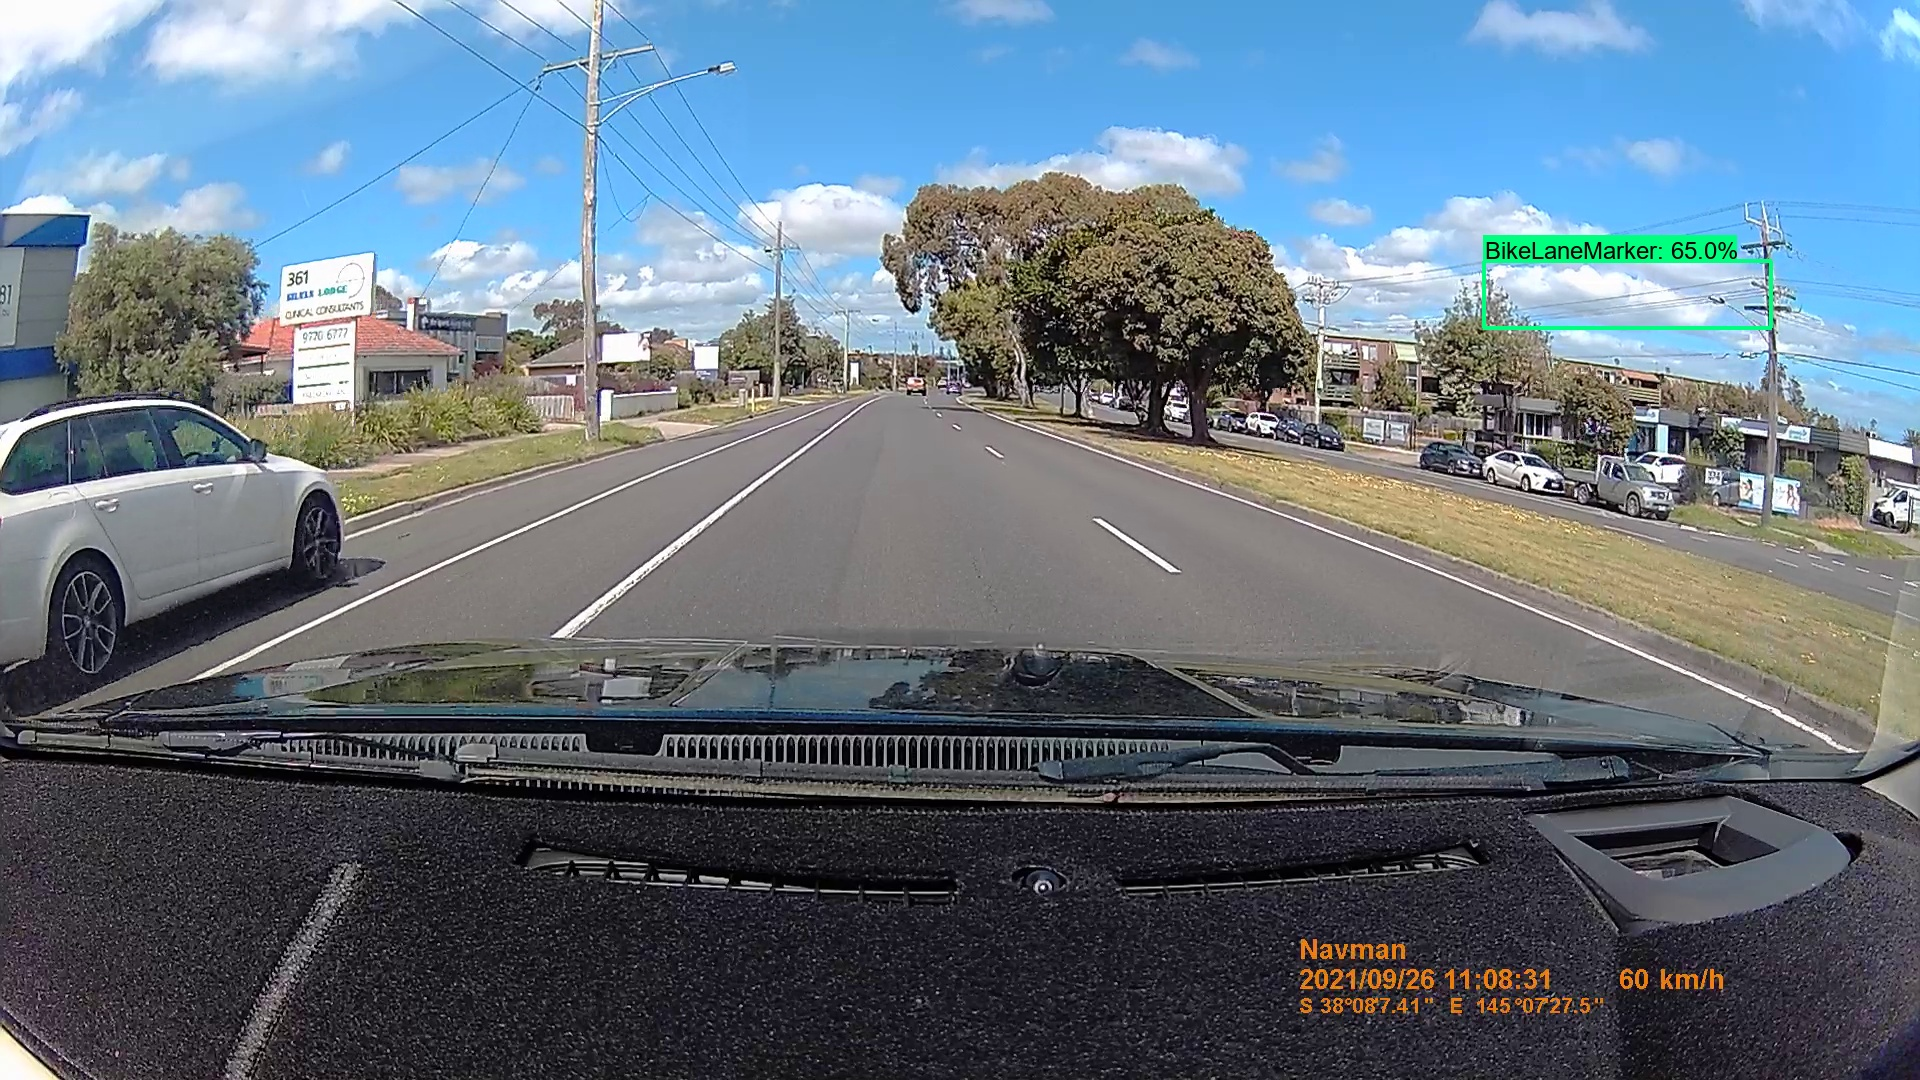
\includegraphics[width=\textwidth]{f005_false_positive_random_sky.jpg}
	\caption{White cloud}
\end{subfigure}
%\hfill
\caption{False Positive Examples}
\label{fig:false_positives}
\end{figure}

A decision was made to re-train the model with selected images from footage that was gathered in a ``training area'' in Frankston, Langwarrin, and Baxter, and to test on independent images gathered in a ``testing area'' in Mount Eliza.  

The footage from the training area was processed through the original Google Street View-trained model as-is, to see where that model was registering detections, whether they be true positives or false positives.  A total of 342 images were selected for labelling so that they could be added to the existing Google Street View images in the dataset.

The original Google Street View training images had been labelled with a single class ``BikeLaneMarker''.  The new training images selected from dash camera footage of the training area were labelled with additional classes, to encourage the model to think of them as something other than a bicycle lane marking.  The following labels were used:

\begin{itemize}
\item{BikeLaneMarker}
\item{GiveWayMarker}
\item{ArrowMarker}
\item{IslandMarker}
\item{RoadWriting}
\item{RoadDefect}
\end{itemize}

Once the new dash camera images had been labelled, they were randomly split 80:20 and added to the Google Street View images in the original training and testing datasets.  The models were then re-trained from scratch based on the combined training dataset, and tested against the new combined test dataset.

The Google Street View images that had already been included in the dataset were \textit{not} re-labelled to consider the additional classes, though this was considered as an option if the influence of the labels in the new dash camera images was insufficient to remove the false positives.  Re-labelling the Google Street View images would have taken a significant amount of time.

To deal with the false positives that had triggered by reflections on the bonnet of the camera vehicle, and random objects on the side of the road, the process was updated to apply a mask to each image before passing it to the detection model.  The mask was designed to exclude the bonnet of the vehicle and anything on the opposite side of the road, and focus attention on places in the frame where a bicycle lane marker might reasonably be encountered in the direction of travel.  See figure \ref{fig:006}.

\begin{figure}[h!]
\centering
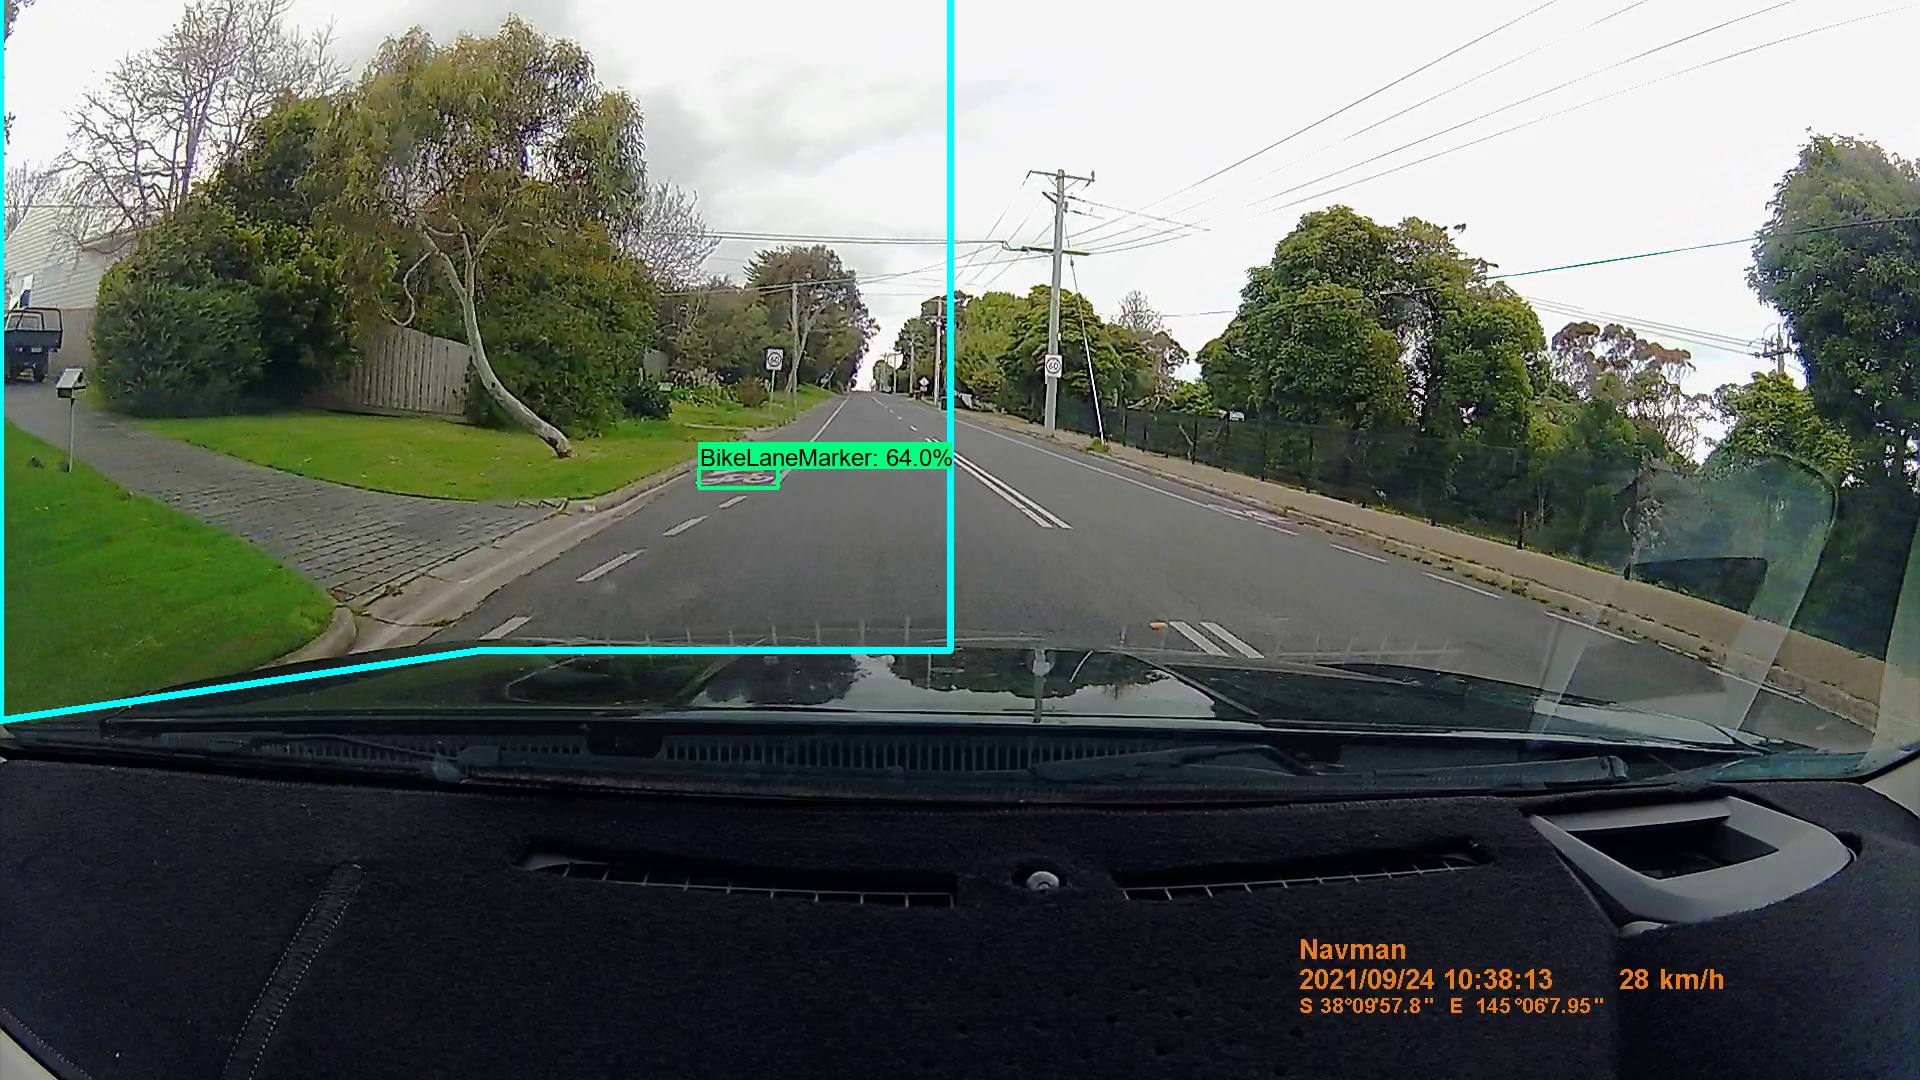
\includegraphics[width=0.5\linewidth]{f006_mask.jpg}
\caption{Detection mask to exclude car bonnet and right hand side of road.}
\label{fig:006}
\end{figure}

The detection model that had been re-trained to include dash camera images from the training area was then evaluated against the independent footage from the testing area in Mount Eliza.


\subsection{Mapping dash camera detections and comparing to other sources}
\label{s:rq3d}

Processing a batch of images from the dash camera yields a CSV file with detection locations.  The location coordinates in this file come from NMEA file, and they may not exactly match ``node'' coordinates from the OpenStreetMap XML data extract.  To produce a map of bicycle lane routes detected from the dash camera footage, we first ``align'' the detection co-ordinates with ``node'' coordinates found in the OpenStreetMap data.  This allows us to more easily compare routes and measure any material differences.

For every detection location logged by the model, we find the nearest ``way'' in the OpenStreetMap XML extract that belongs to a named road.  The Python ``shapely'' library helps us to perform this search as efficiently as possible, using bounding boxes for each way to avoid a brute force search of all points.  Once we have found the nearest ``way'', we check every ``node'' in the way to record the nearest \textit{intersection} ``node'', and the nearest ``node'' of \textit{any type}.  We consider there to be a ``hit'' at the coordinates of both nodes:  the point on the OpenStreetMap route closest to the detection -- which may a bicycle lane marking that occurs at intervals of up to 200 metres along the road \cite{standards} -- and the closest intersection along the road.

Once the detection coordinates have been aligned to the OpenStreetMap coordinates, geojson files can be ``drawn'' and compared to other sources using the same techniques as for the Google Street View images.  This route inference process is based entirely on the nearest intersection for each detection, but preserving the co-ordinates of the nearest ``node'' of any type in the output helps with traceability.


% ~~~~~~~~~~~~~~~~~~~~~~~~~~
\section{RQ4: Surveying other infrastructure details using dash camera footage}

Once dash camera footage had been used to map bicycle lane routes in a survey area, some further work was conducted to demonstrate how the approach might be re-used to survey other details of interest.  To demonstrate future potential, a process was created to map any paved shoulders on the side of the roads in the survey area that cyclists might ride on achieve physical separation from motor vehicles.  Previous studies such as Klobucar \& Fricker, 2007 \cite{BIKESAFETY} have observed that a paved shoulder can improve cyclist safety, even if it is not formally marked as a bicycle lane.

For a discussion of other areas of potential for future work, please refer to section \ref{s:future_work}.

To identify a paved shoulder, it is necessary to detect lane markings, and the edge of the road if it is not explicitly marked.  We are interested in the edge of the road on the side of the road that traffic usually drives on.  In this research, dash camera footage was captured in Australia, so we are interested in the left hand side.  The following text therefore refers to the edge of the road on the side that traffic usually drives on as the ``left''.


\subsection{Correcting for lens distortion}

Lens distortion is where the optical properties of a camera's lens causes straight lines to appear curved in an image.  The ``OpenCV'' library provides a method to correct distortion for a specific camera \cite{distortion}.  The camera is used to capture a range of images where a special calibration tool appears in frame.  See figure \ref{fig:calibration} for some example images.  An image of a ``chessboard'' pattern of known dimensions is held in front of the camera in different positions.

\begin{figure}[h]
\centering
\begin{subfigure}{0.24\textwidth}
	\includegraphics[width=\textwidth]{f007_calibration1.png}
\end{subfigure}
\hfill
\begin{subfigure}{0.24\textwidth}
	\includegraphics[width=\textwidth]{f007_calibration2.png}
\end{subfigure}
\hfill
\begin{subfigure}{0.24\textwidth}
	\includegraphics[width=\textwidth]{f007_calibration3.png}
\end{subfigure}
\hfill
\begin{subfigure}{0.24\textwidth}
	\includegraphics[width=\textwidth]{f007_calibration4.png}
\end{subfigure}
\caption{Example OpenCV camera calibration images}
\label{fig:calibration}
\end{figure}

After the calibration images are collected, they are processed by OpenCV to create a mathematical model of the camera's lens distortion.  With this model, OpenCV can apply a transformation to images from the same camera, to correct for lens distortion.

When searching for paved shoulders in a survey area, we are looking for lines in an image that are often straight.  The dash camera being used to collect images was therefore calibrated, and in this exercise, all images were processed to correct for distortion.  See figure \ref{fig:008} for an example raw image from the dash camera, and a corresponding corrected version.

\begin{figure}[h]
\centering
\begin{subfigure}{0.45\textwidth}
	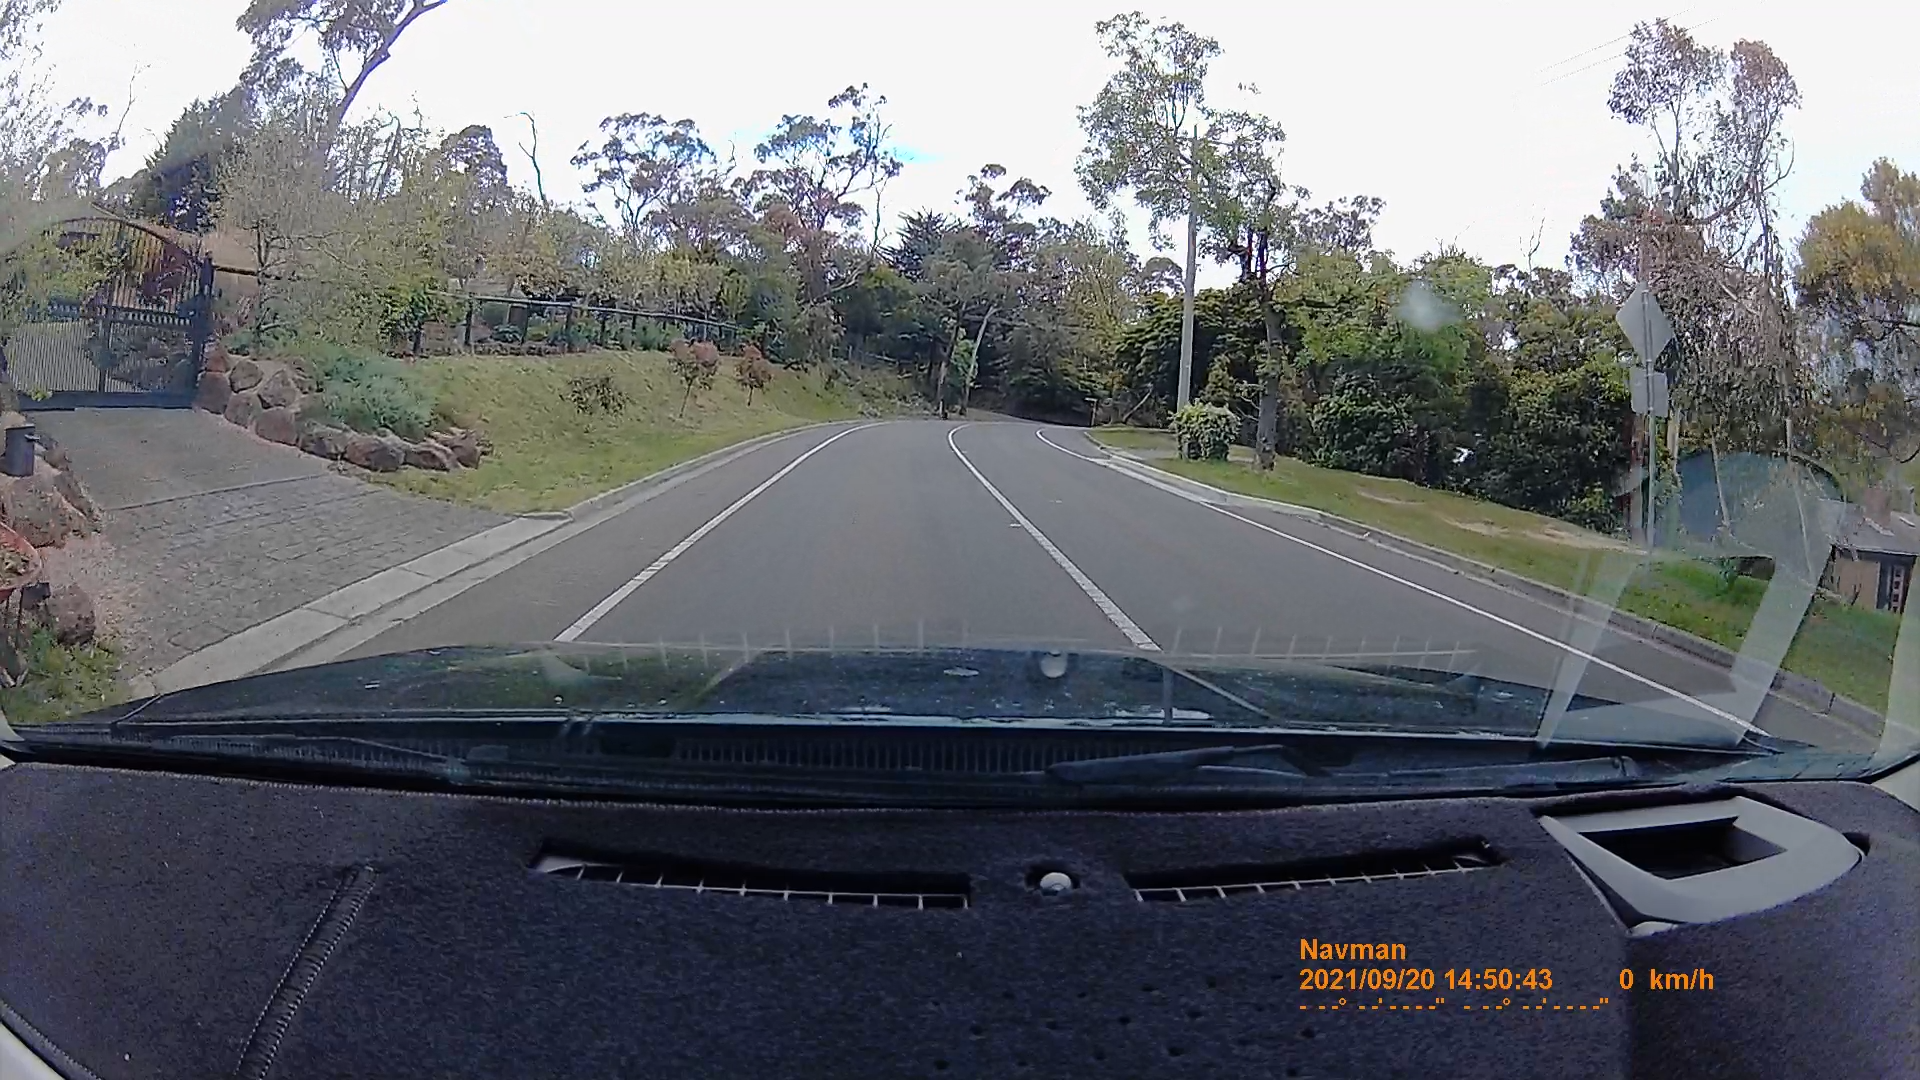
\includegraphics[width=\textwidth]{f008_uncorrected.png}
	\caption{Uncorrected image}
\end{subfigure}
\hfill
\begin{subfigure}{0.45\textwidth}
	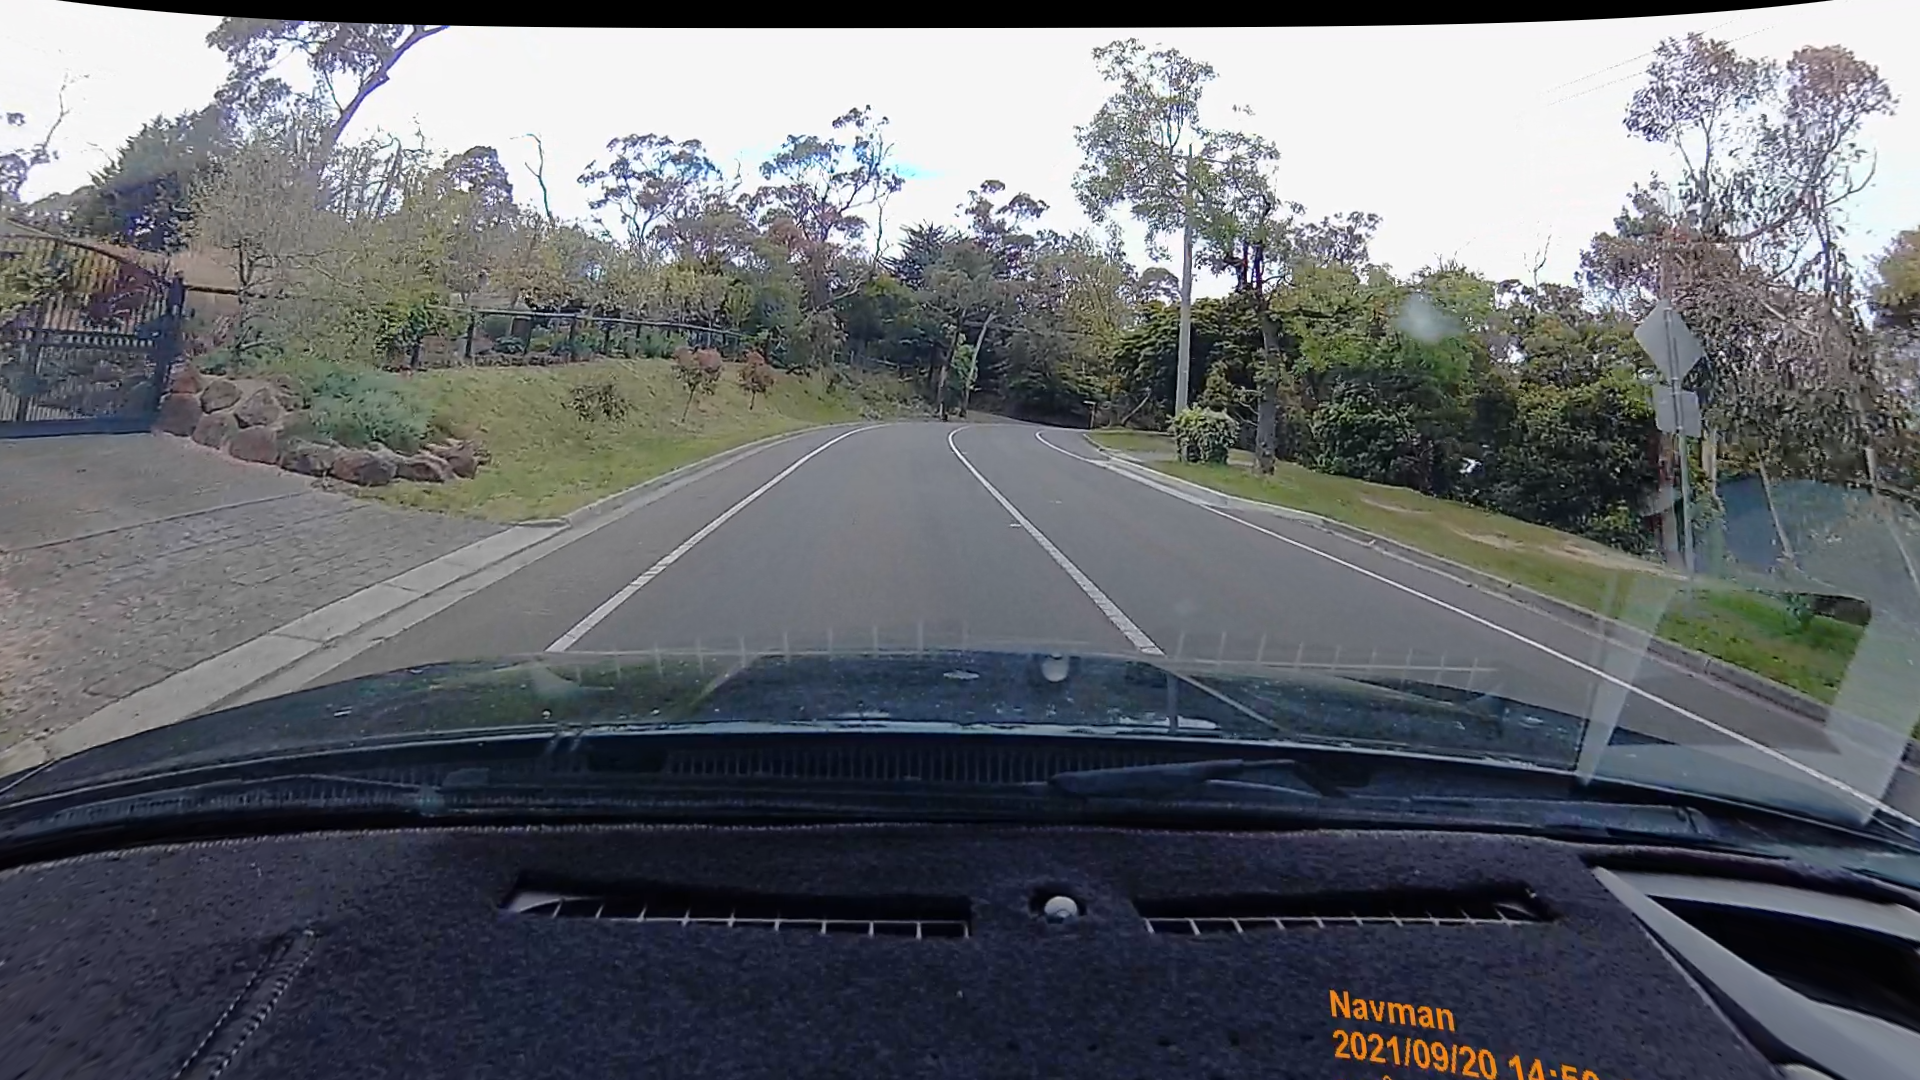
\includegraphics[width=\textwidth]{f008_corrected.png}
	\caption{Corrected image}
\end{subfigure}

\caption{Example OpenCV camera calibration images}
\label{fig:008}
\end{figure}

The most obvious sign that the correction has been applied in this example is that the top edge of the corrected image is bent downwards slightly, and the location/speed/time information that usually appears in the bottom right corner has been shifted.


\subsection{Detecting lane markings}

A common solution to the problem of detecting lane markings involves applying a combination of the Canny edge detection algorithm proposed by Canny, 1987 \cite{canny} and the Hough transformation proposed by Hough, 1972 \cite{hough}.  This general approach has been followed in many papers such as Li et al, 2016 \cite{canny_example} and Chai et al, 2014 \cite{canny_example2}, and it is frequently used in capstone projects in the self-driving car domain.  At its most basic, the approach does not involve any machine learning or deep learning techniques.

The Canny/Hough approach typically works as follows:

\begin{itemize}
\item{Convert the image to greyscale}
\item{Apply Canny edge detection to detect edges in an image \cite{canny}}
\item{Apply a mask to exclude edges outside a triangle representing the area immediately in front of the vehicle}
\item{Apply a Hough transform \cite{hough} to convert these edges into lines, each line having a slope and an intercept.}
\item{Partition the lines into two groups:  Lines that slope upwards from left to right, and lines that slope downwards from right to left.}
\item{For each group of lines, take the average slope and intercept.  These represent the assumed lane boundaries.}
\item{Use the slope and intercept of each detected line to overlay a line on the original image, extending from the bottom of the image to a suitable ``horizon'' somewhere around half-way to the top of the image.  These straight lines representing the lane boundaries can be visualized by superimposing them over the original image.}
\end{itemize}

Please see figure \ref{fig:009} for example images to demonstrate the process.

\begin{figure}[h]
\centering
\begin{subfigure}{0.4\textwidth}
	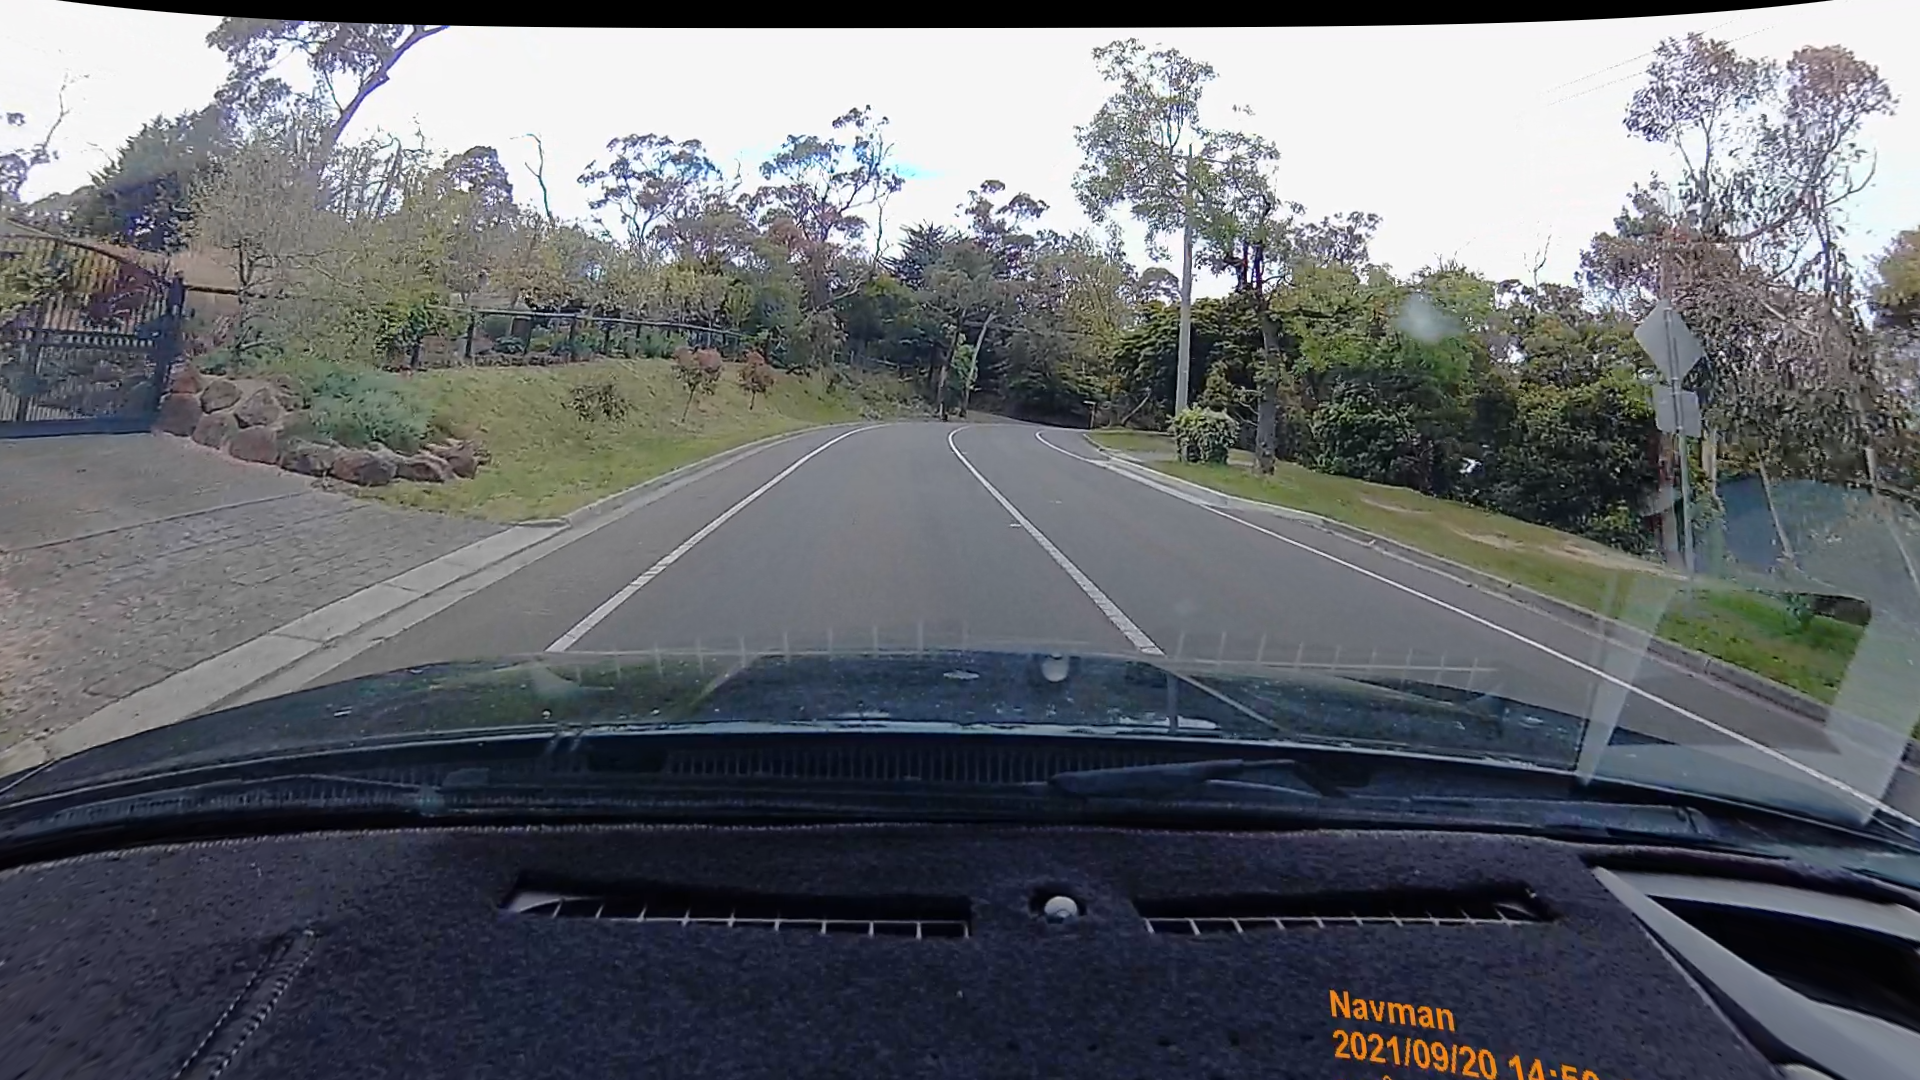
\includegraphics[width=\textwidth]{f008_corrected.png}
	\caption{Corrected image}
\end{subfigure}
\hfill
\begin{subfigure}{0.4\textwidth}
	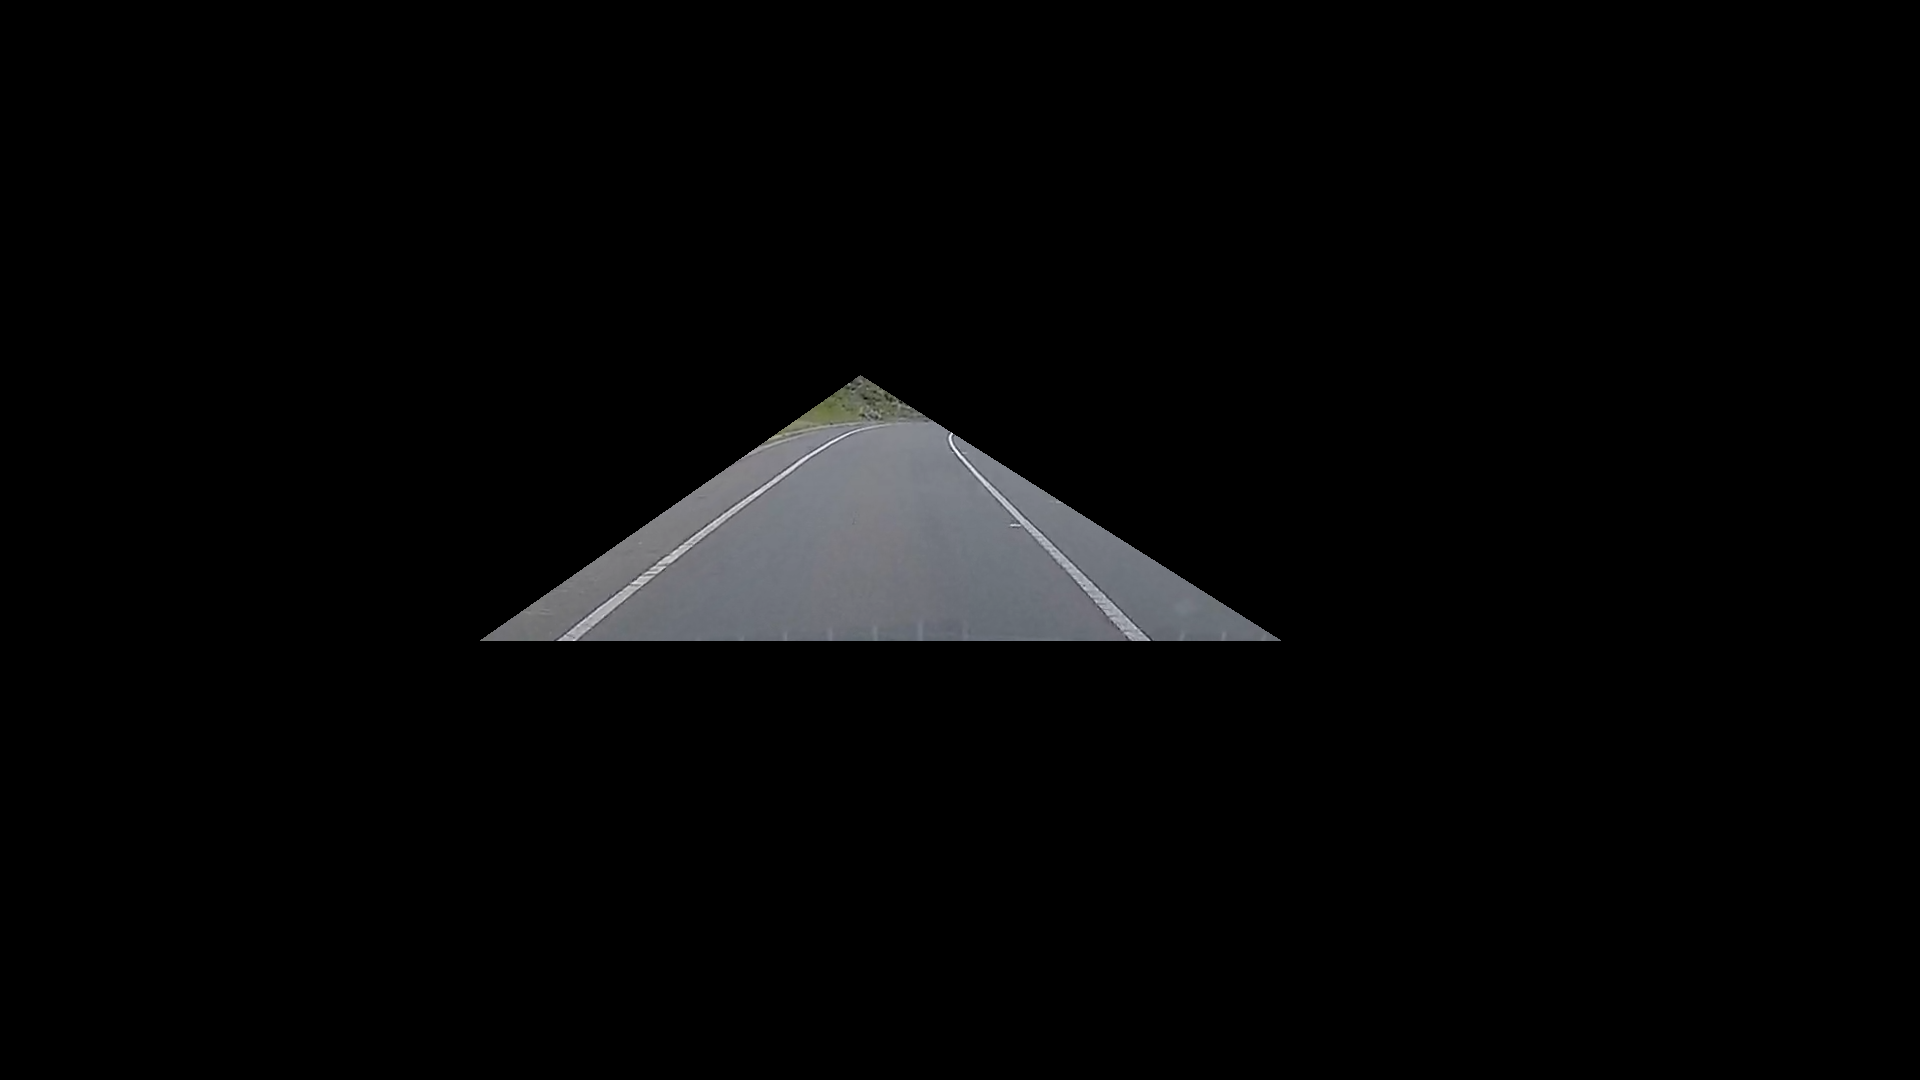
\includegraphics[width=\textwidth]{f009_original_cropped.png}
	\caption{Proposed mask}
\end{subfigure}
\hfill
\begin{subfigure}{0.4\textwidth}
	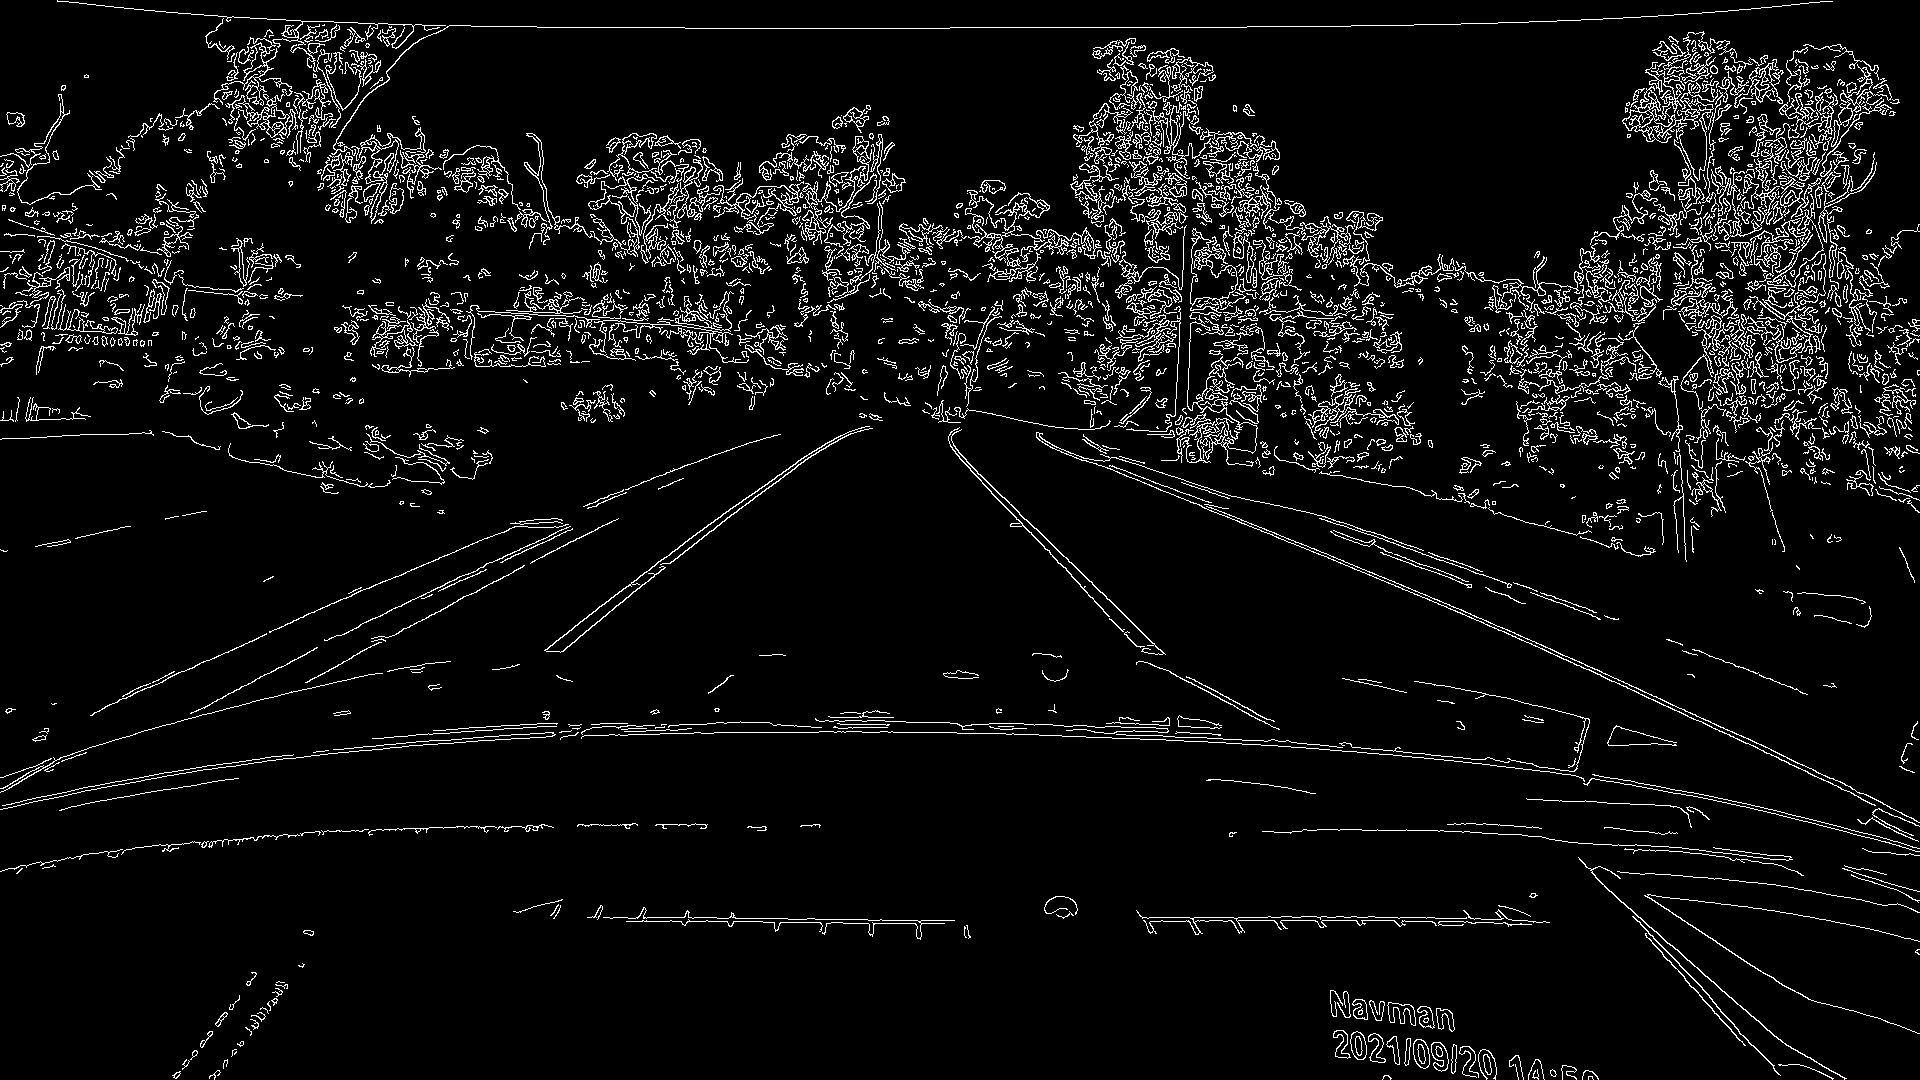
\includegraphics[width=\textwidth]{f009_canny.png}
	\caption{Canny edge detection}
\end{subfigure}
\hfill
\begin{subfigure}{0.4\textwidth}
	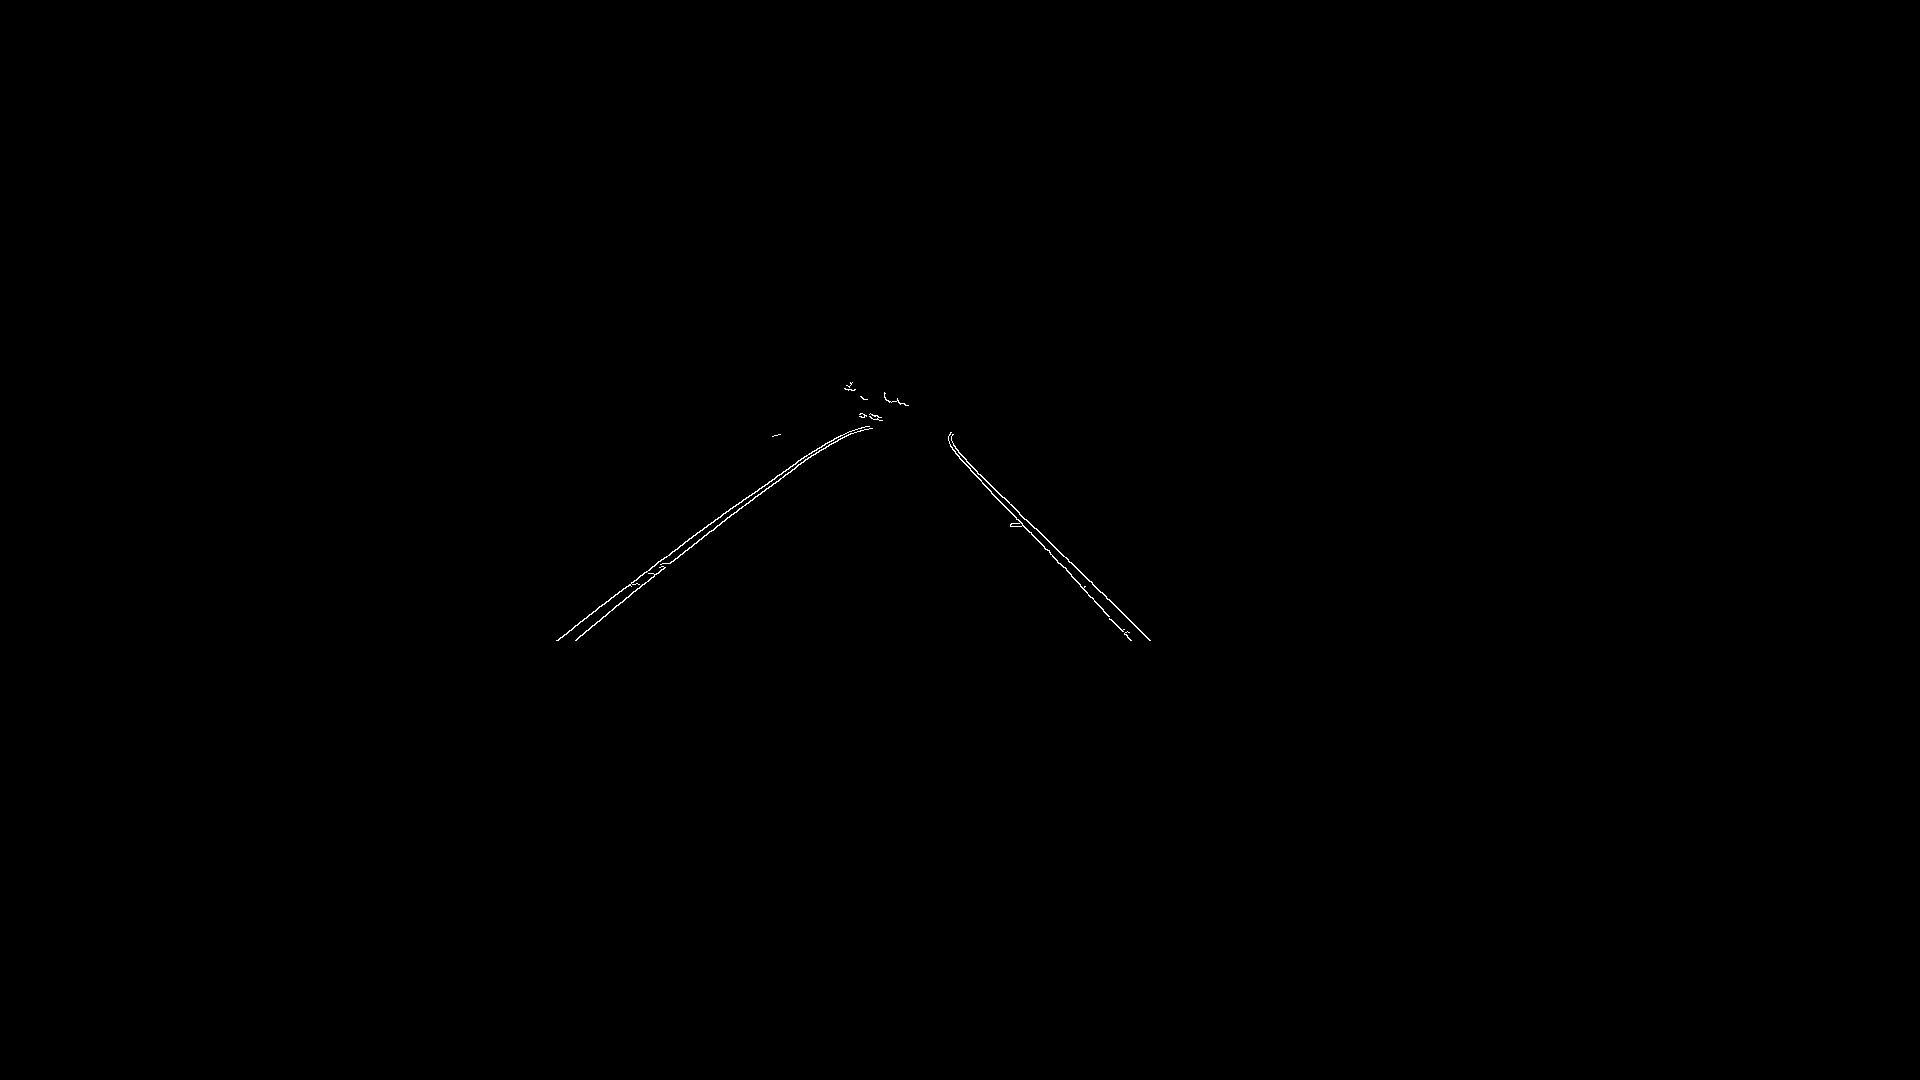
\includegraphics[width=\textwidth]{f009_canny_cropped.png}
	\caption{Mask applied to Canny edge detection}
\end{subfigure}
\hfill
\begin{subfigure}{0.4\textwidth}
	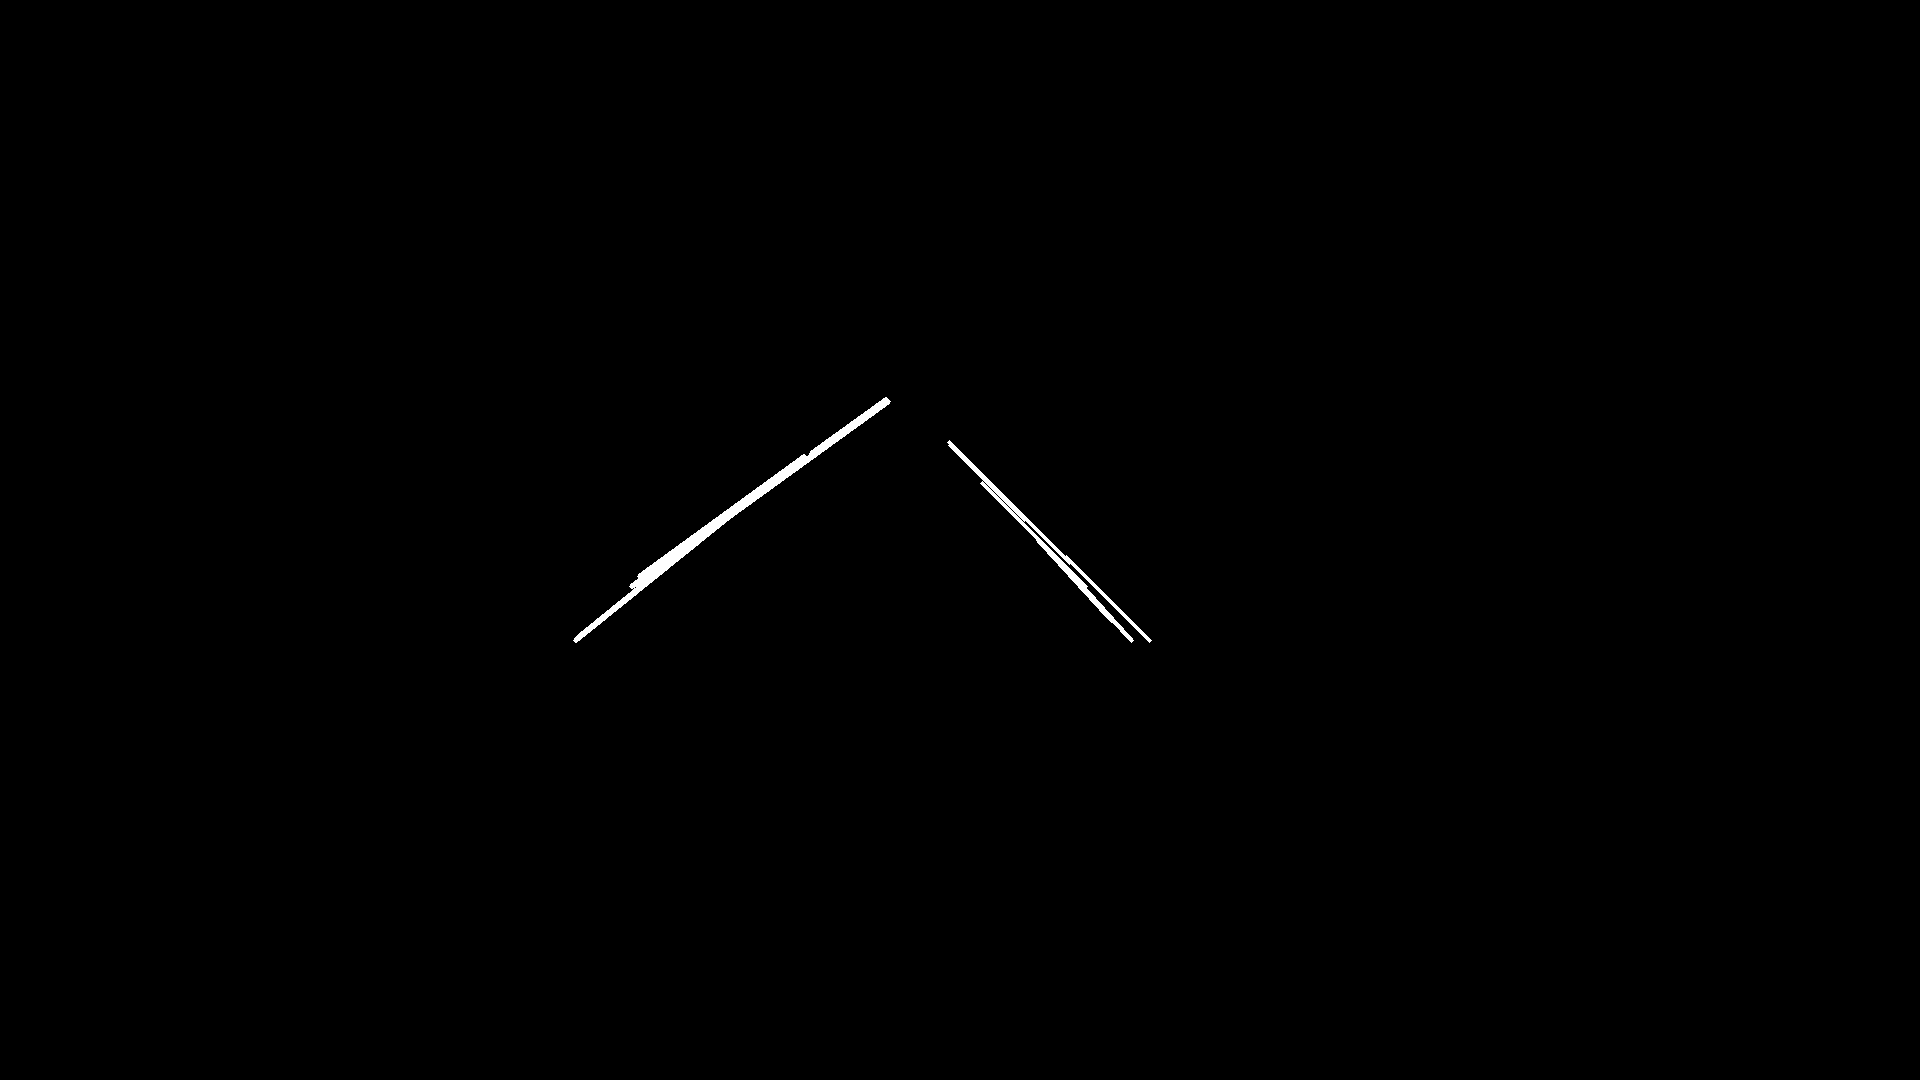
\includegraphics[width=\textwidth]{f009_hough.png}
	\caption{Hough transform}
\end{subfigure}
\hfill
\begin{subfigure}{0.4\textwidth}
	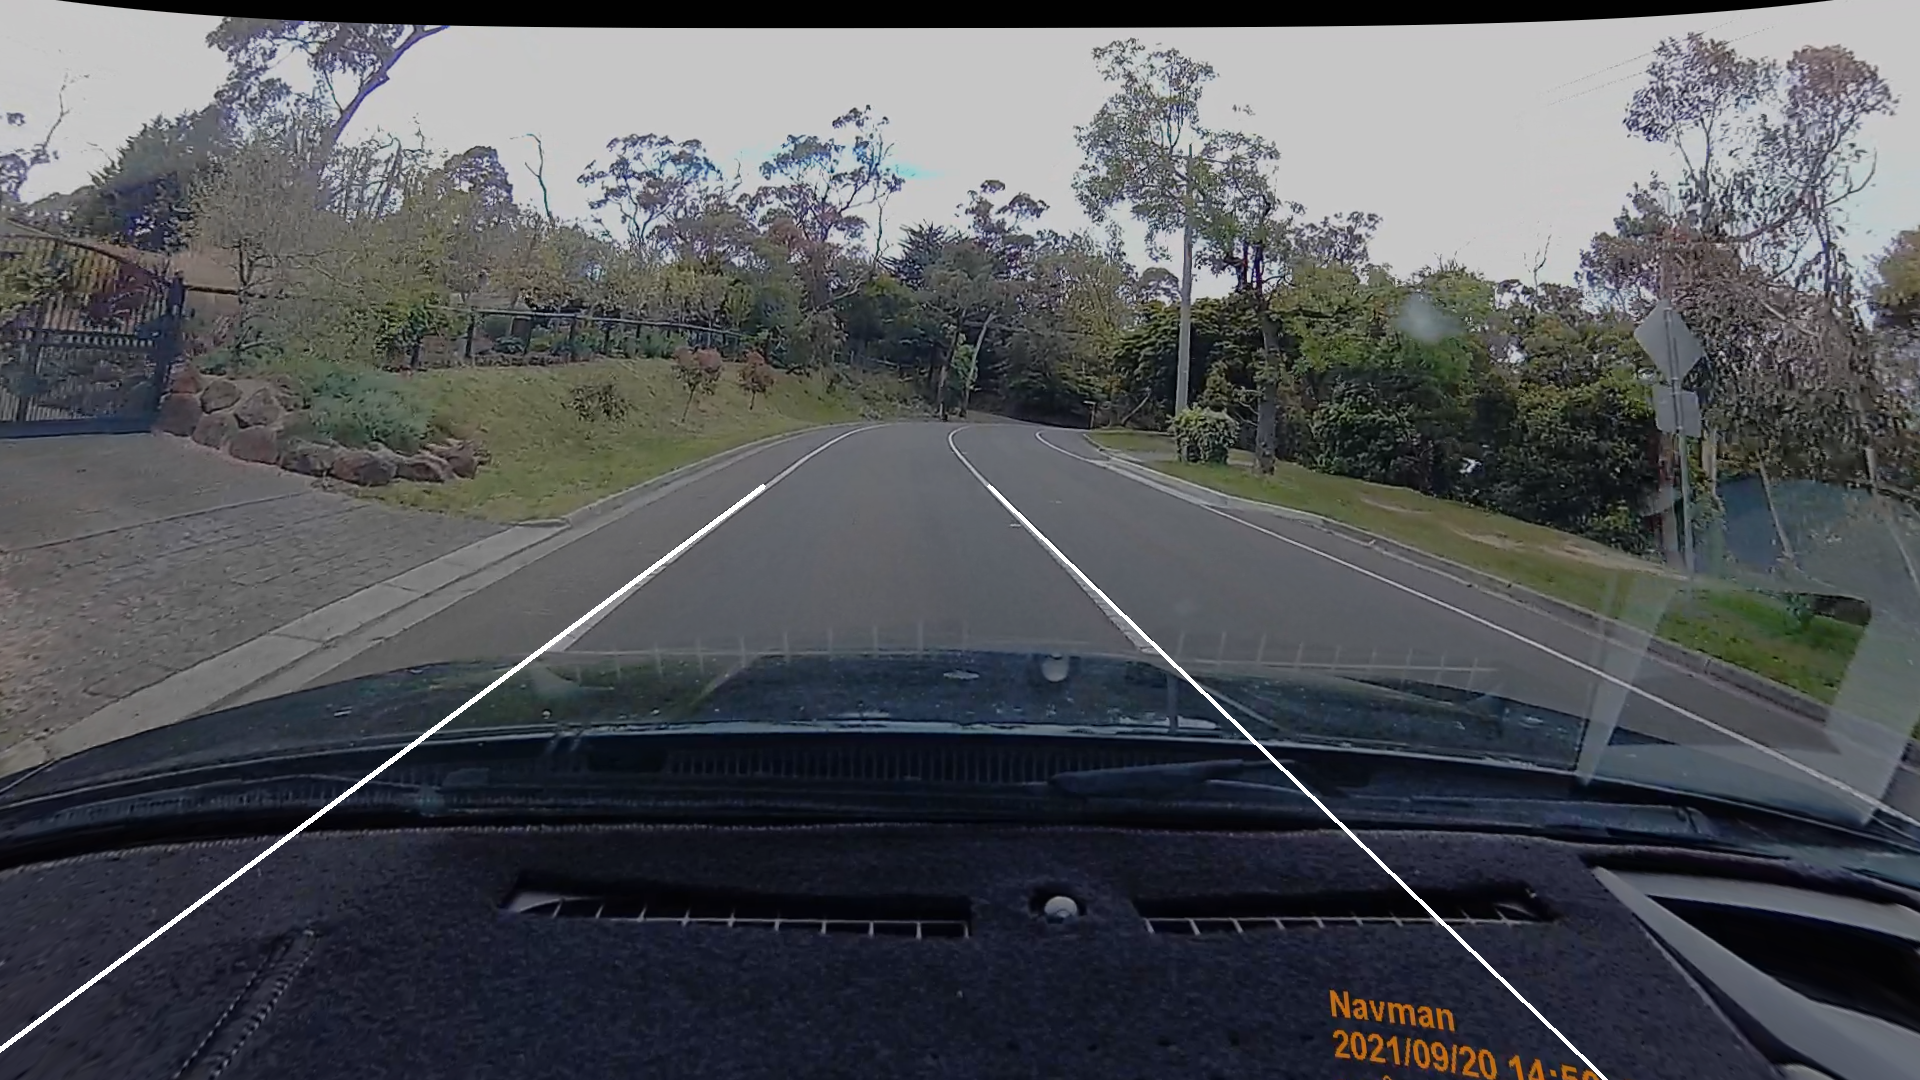
\includegraphics[width=\textwidth]{f009_own_lane.png}
	\caption{Average lines, superimposed}
\end{subfigure}
\caption{Example sequence of Canny/Hough operations to detect own lane}
\label{fig:009}
\end{figure}

The ``OpenCV'' library provides convenient tools to implement the required transformations.

Typically, the Canny/Hough process is used to detect the camera vehicle's own lane.  In order to detect a paved shoulder, we first want to detect the boundaries of our vehicle's own lane, then perform a second pass at the image where the mask has shifted to focus exclusively on areas to further to the edge of the road.

A paved shoulder will be defined by two lines, each with a ``slope'' and an ``intercept''.  One line will be the left boundary of the camera's own lane, which is also the right boundary of the paved shoulder.  The other line will be the left boundary of the paved shoulder, further to the edge of the road.  To detect this third line, we apply a mask to the Canny edge detection image just to the left of the camera's own lane that was found in the first step.  We then apply the same Hough transformation to detect lines, and average the ones with the expected ``left'' slope, to find a slope and intercept for the outer boundary of the paved shoulder.  See figure \ref{fig:010}.

\begin{figure}[h]
\centering
\begin{subfigure}{0.3\textwidth}
	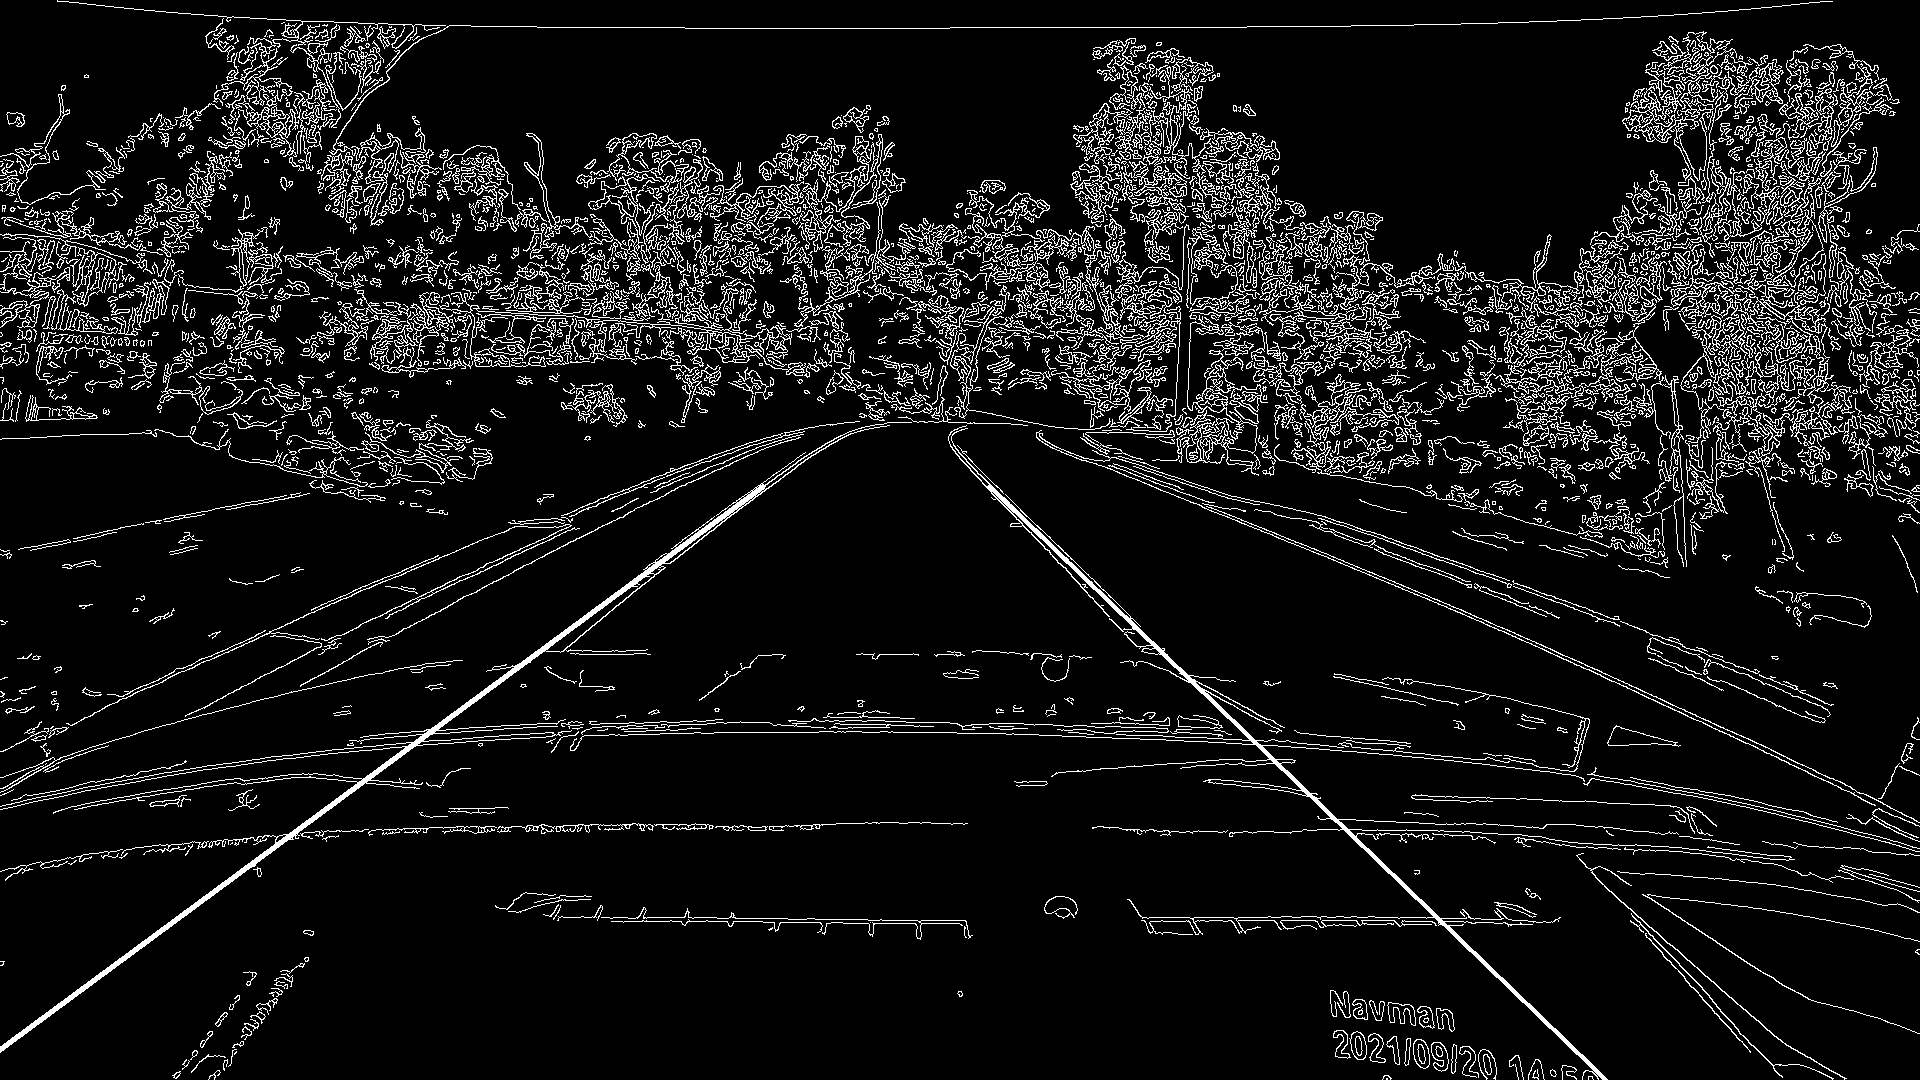
\includegraphics[width=\textwidth]{f010_canny_super.png}
	\caption{Canny edge detection with previously detected lane}
\end{subfigure}
\hfill
\begin{subfigure}{0.3\textwidth}
	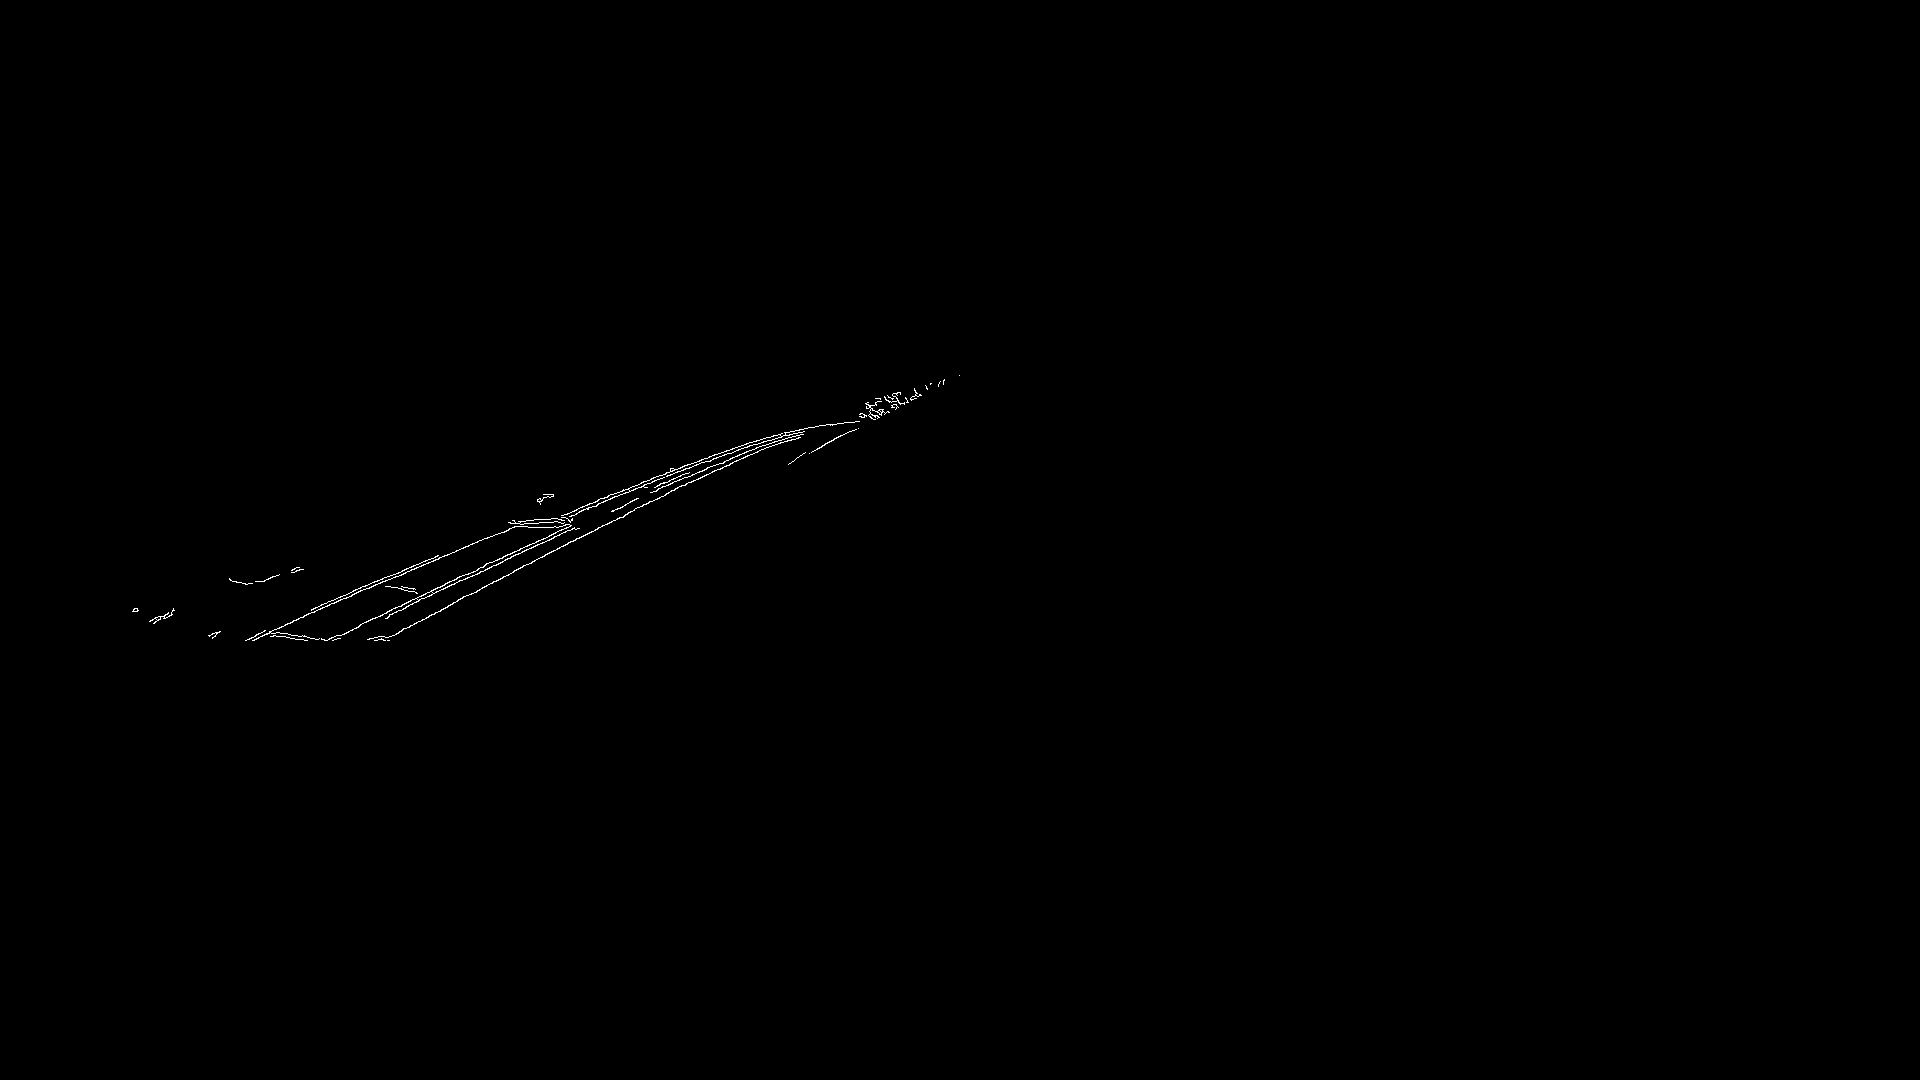
\includegraphics[width=\textwidth]{f010_canny_mask.png}
	\caption{Canny edges with new mask applied}
\end{subfigure}
\hfill
\begin{subfigure}{0.3\textwidth}
	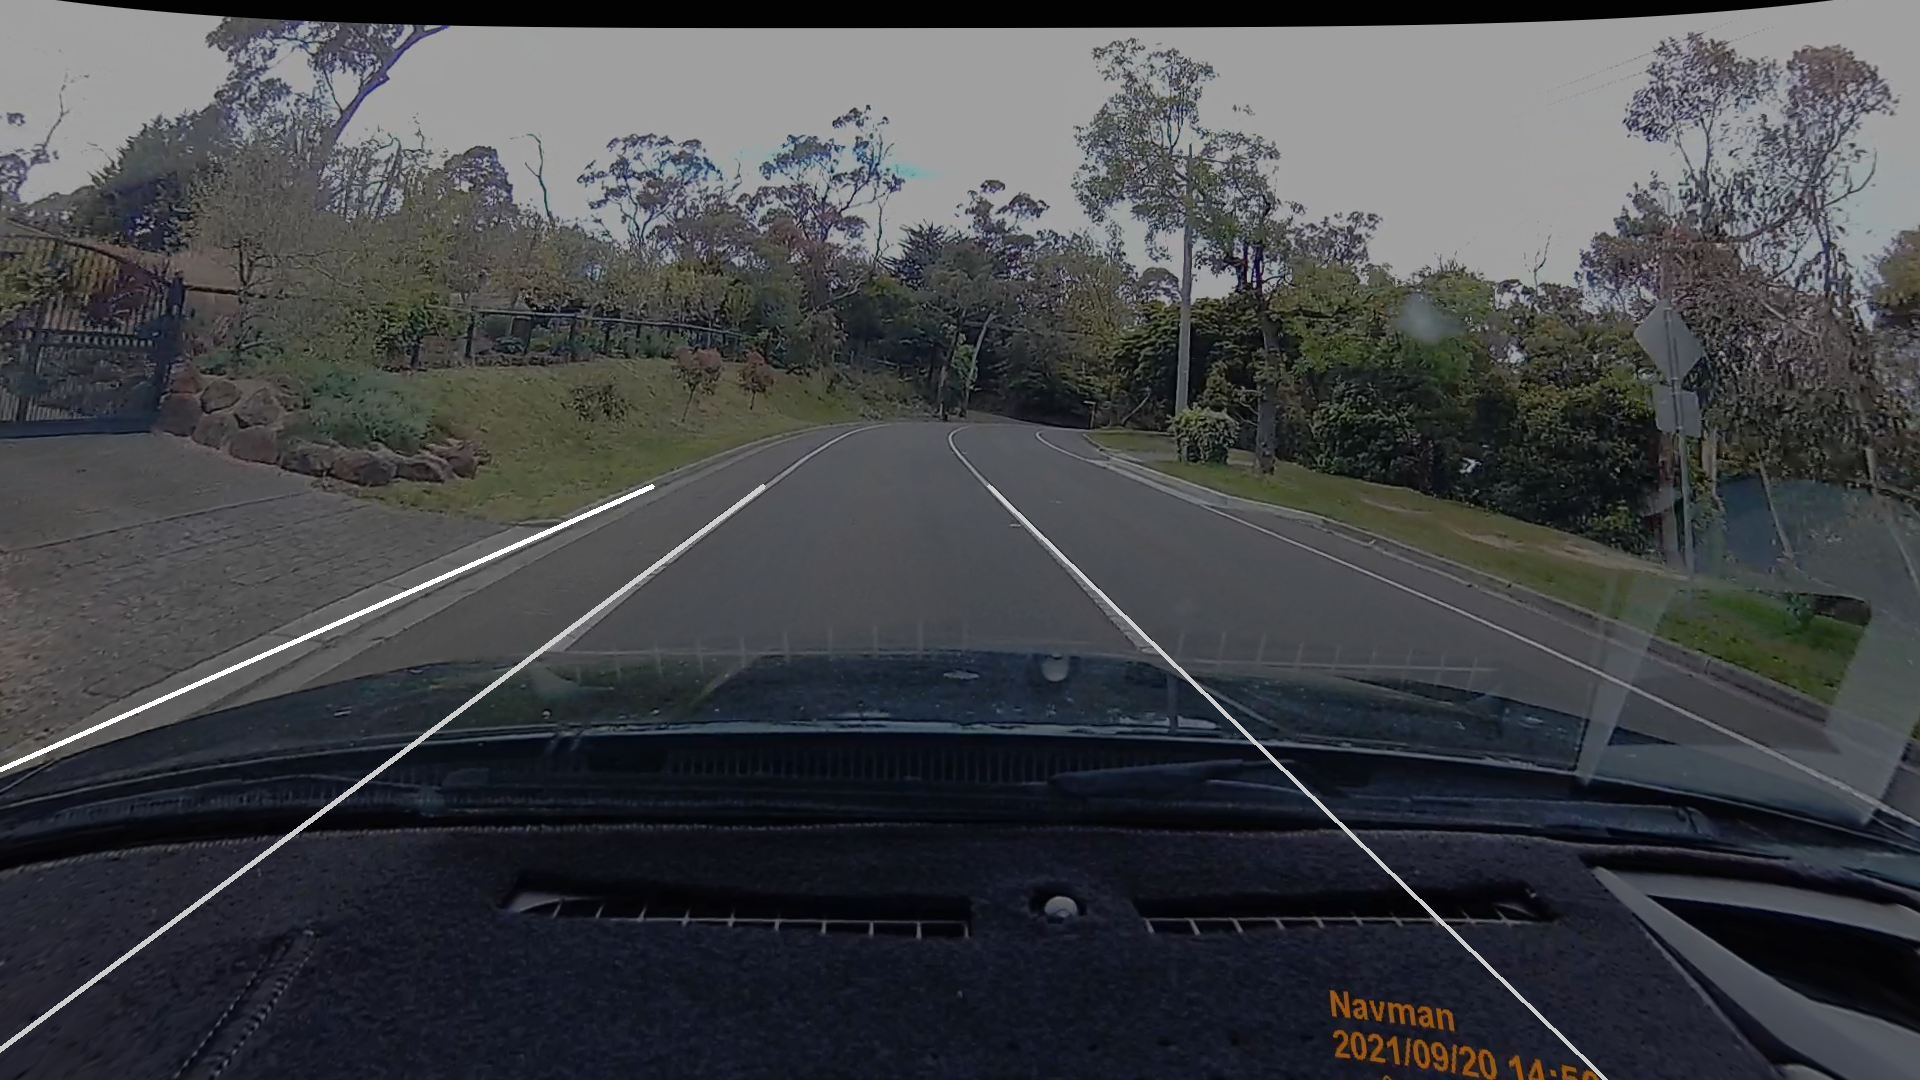
\includegraphics[width=\textwidth]{f010_three_lines.png}
	\caption{Image with all three detected lines}
\end{subfigure}
\caption{Example sequence of Canny/Hough operations to detect paved shoulder}
\label{fig:010}
\end{figure}


If the Canny/Hough approach cannot find another line to the left of our the camera vehicle's own lane, it is a strong sign that there is no clearly defined paved shoulder on the road at that location.  If a line is found, it could be a paved shoulder, or it could be a false positive caused by ``noise'' from something on the side of the road, but within the area included by the mask.

Please see figure \ref{fig:011} below for example images where lines were detected for a possible paved shoulder.  In each of the example figures, two horizontal lines have been drawn, to highlight where the detected lines intersect the a height just above the bonnet of the car, and a height further into the distance, closer to the ``horizon'' of the mask.

\begin{figure}[h]
\centering
\begin{subfigure}{0.3\textwidth}
	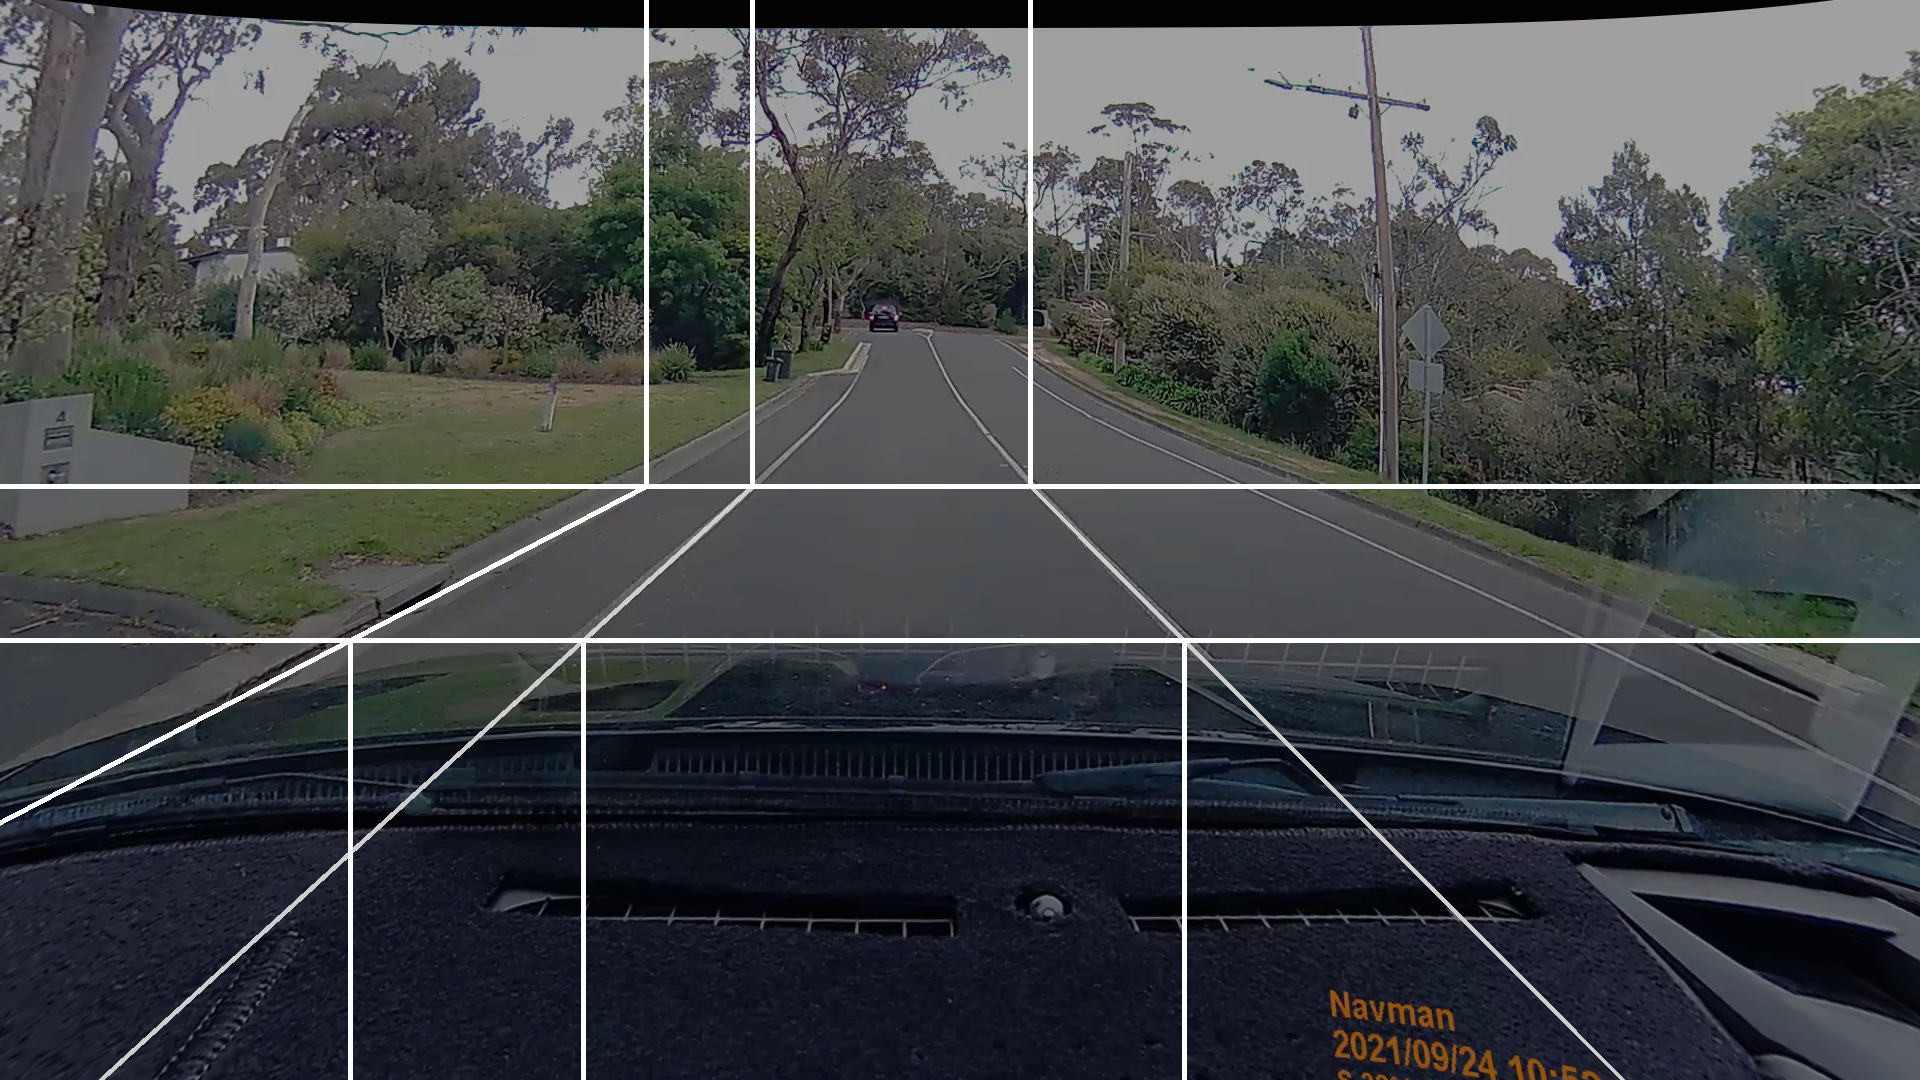
\includegraphics[width=\textwidth]{f011_true.png}
	\caption{A paved shoulder has been correctly identified}
	\label{fig:011a}
\end{subfigure}
\hfill
\begin{subfigure}{0.3\textwidth}
	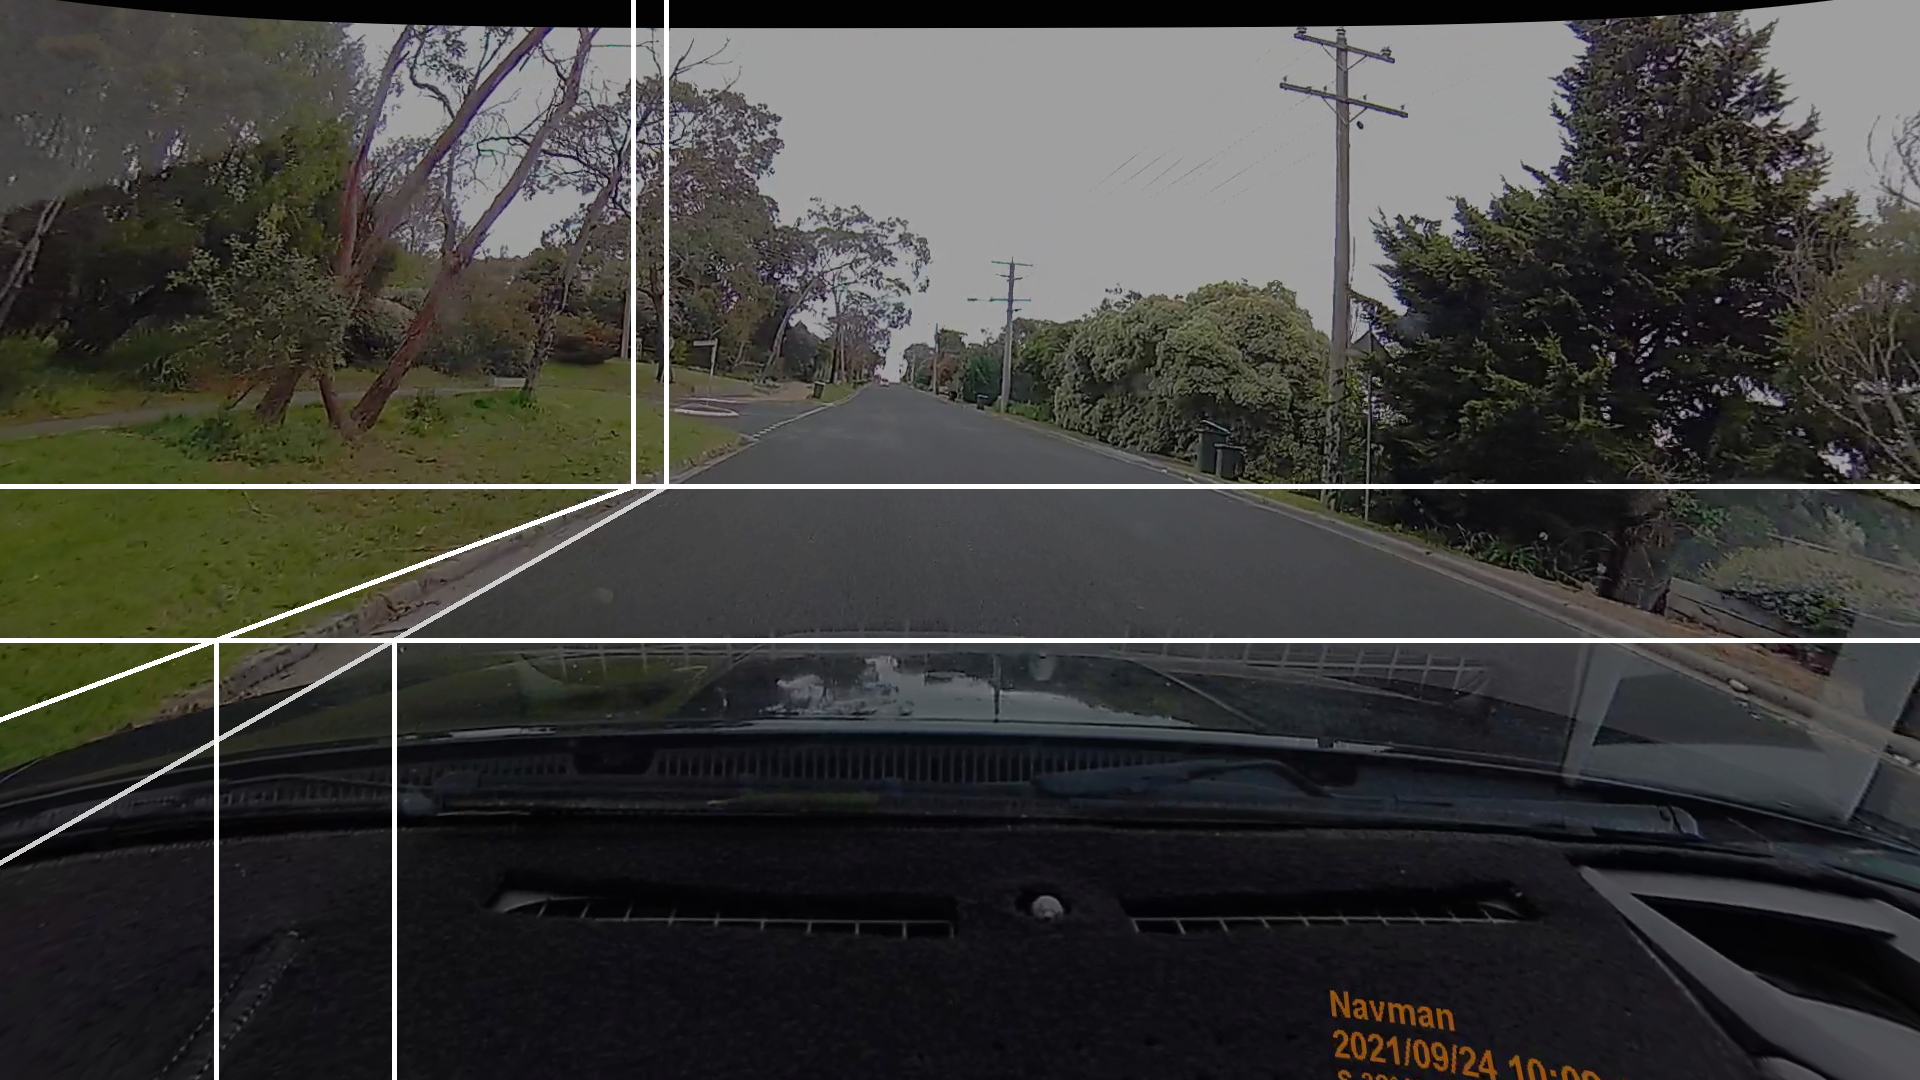
\includegraphics[width=\textwidth]{f011_false_gutter.png}
	\caption{A gutter has resulted in a very narrow shoulder area}
	\label{fig:011b}
\end{subfigure}
\hfill
\begin{subfigure}{0.3\textwidth}
	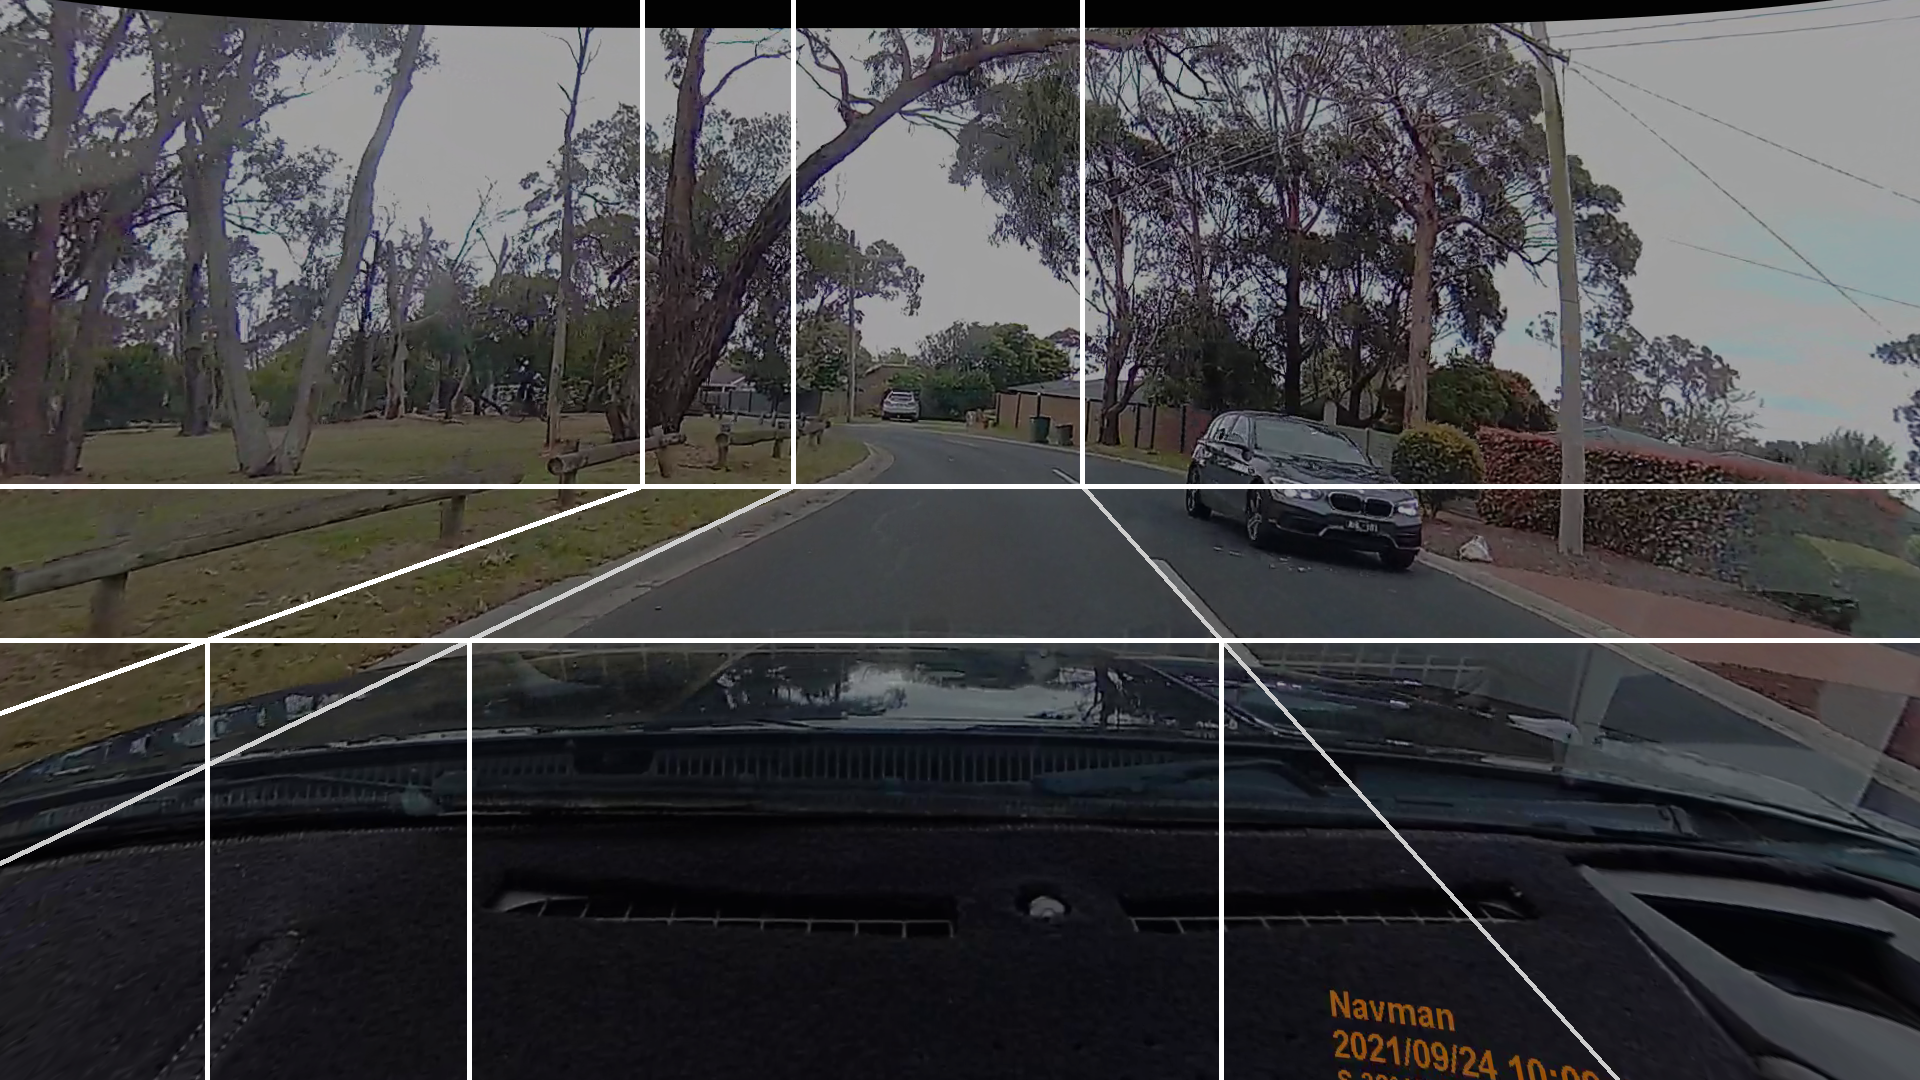
\includegraphics[width=\textwidth]{f011_false_fence.png}
	\caption{``Noise'' from the straight lines in a fence}
	\label{fig:011c}
\end{subfigure}
\caption{Example paved shoulder detections}
\label{fig:011}
\end{figure}

Figure \ref{fig:011a} shows a true positive match, where the boundaries of a paved shoulder have been correctly identified.

Figure \ref{fig:011b} shows a situation where a concrete gutter has resulted in a very narrow area being detected.  This potential false positive can be mitigated by requiring a minimum width for any detected area.

Figure \ref{fig:011c} shows a false positive match, where ``noise'' from a park fence parallel to the road has caused the average of lines to the left of the camera's old lane to appear to be a paved shoulder.  However, this phantom line is not ``stable'' and only appears for a few frames.  This type of false-positive can be reduced using metrics that require a line to appear consistently across most images in a road segment, and/or requiring that the slope and position of the line not vary too much from frame to frame.


\subsection{Mapping paved shoulders across a survey area}

The Canny/Hough lane detection method can be applied to all sample frames from the survey area, using a similar batch process to the bicycle lane detection process in section \ref{s:rq3} and substituting a different detection model.  The challenge is setting robust criteria for flagging a ``detection'' that will result in a sensible map.  The simplest criteria would be to look for frames where lines were detected for both the left and right boundaries of a paved shoulder.  This criteria was applied to the training area footage, and the resulting images with detection line overlays were reviewed in chronological order.  The results were very inconsistent.

Reviewing the footage, it was found that on roads where there was a paved shoulder or bicycle lane, the boundaries of that lane remained relatively stable from frame to frame, and the width of gap between the boundaries towards the ``horizon'' at the top of the frame was relatively wide.  There were relatively few ``skipped'' frames where the boundaries were not detected.  In contrast, on roads without a paved shoulder or bicycle lane, there may be many ``skipped'' frames, the slopes of the detected boundaries were much less consistent from frame-to-frame, and the detected boundary lines often had an intersection point much closer to the bottom of the frame.

The following solution was proposed:

\begin{itemize}
\item{Each frame would be linked to its two nearest intersection ``nodes'' in the  OpenStreetMap data.  Frames associated with a single stretch of road between two intersections would be assessed as a group, to determine whether a paved shoulder or bicycle lane exists along that stretch.}
\item{Frames from locations within 30 metres of an intersection were excluded from consideration, because it is common for them to ``disappear'' at the approach to an intersection, and this disappearance should not counted as a missed detection.}
\item{If the model fails to find both boundaries of a paved shoulder in more than 20\% of the remaining frames along a stretch of road, then it is assumed that there isn't one.}
\item{A horizontal line is drawn across the frame towards a ``horizon'' as per figure \ref{fig:011}.  The width of the space between the boundary lines is measured at this height within the frame, in pixels.  The mean width is calculated across all frames in the stretch of road where boundary lines were detected.  If the mean is less than 75 pixels, then the possible paved shoulder is too narrow, and it is assumed not to exist.  This accounts for very narrow margins such a gutter that are of no use to a cyclist.}
\item{If the model finds both left and right boundary lines for a possible paved shoulder, use the slopes and intercepts to calculate an (x,y) coordinate relative to the bitmap image where those two boundary lines intercept.  Calculate the standard deviation of the x and y intersection values across all frames in the stretch of road where both boundary lines are defined.  If the standard deviation in either the x or y dimension is greater than 50 pixels, then the boundary lines are considered to be too inconsistent across images.  The stretch of road is assumed not to have a paved shoulder.}
\end{itemize}

The thresholds described above were set based on the following process:

\begin{itemize}
\item{Update the batch process to output a row for every frame, in chronological order}
\item{Include the name of the road for traceability.}
\item{Include the node IDs of the two nearest intersections, to trace which frames are part of the same group.  The first node ID is the one that comes first alphabetically, not the one that is closest to the location associated with the frame.  This is to avoid splitting a group of frames for a stretch of road into two groups depending on which intersection is closest.}
\item{Filter out frames where the location is within 30m of either of the two nearest intersections}
\item{Create summary statistic columns for each group for frames, and add them to the output CSV as additional columns:
	\begin{itemize}
	\item{Proportion of frames where boundary lines were not detected}
	\item{Mean width of the potential paved shoulder, in pixels, at the horizontal ``horizon'' line}
	\item{Standard deviation of the y-coordinate where the boundary lines intersect}
	\item{Standard deviation of the x-coordinate where the boundary lines intersect}
	\end{itemize}
}
\item{Apply this process to the training area footage to produce an output CSV.}
\item{Load the output CSV file into an editor, and add a ``truth'' column to denote whether a paved shoulder really exists at each location, based on a manual review of the output frames with the detection line overlay.}
\item{Filter the data to find thresholds in the summary statistics that appear to explain how the ``truth'' values are partitioned, as closely as possible.}
\item{Create ``prediction'' column in the output CSV based on the chosen thresholds, and compare it to the ``actual'' value in the ``truth'' column.}
\end{itemize}

The model was then applied to the footage from the Mount Eliza testing area to see how it performed with the selected thresholds.

To construct a map of detected paved shoulders, take the distinct combinations of ``way'' ID and the ``node'' IDs of the two closest sections, where a paved shoulder was predicted.  Find the ``way'' ID in the OpenStreetMap data, and ``draw'' a ``LineString Feature'' in a geojson file for all ``nodes'' between the two intersection nodes, including the intersection nodes themselves.  The geojson file can then be drawn on map in a Jupyter Notebook using the Python ``ipyleafelet'' library as per sections \ref{s:rq2} and \ref{s:rq3}.

In this exercise, lane detection was attempted from the dash camera footage only,  as a demonstration of how the techniques developed to address the first three research questions could be re-used to gather other information visually.  It could be applied to Google Street View images, however it was only attempted with the dash camera footage where it is easier to ensure that each image is taken with a heading that is consistent with the direction of the road.  The application of the Canny/Hough approach to lane detection across a variety of environments is challenging, and could be considered a separate research project in itself.  To get a more consistent detection of the road boundary in the face of road-side ``noise'', it would be worth exploring deep learning image segmentation techniques to train a model that can detect the road surface, similar to the approach taken by Mamidala et al., 2019 \cite{8929655}.  It would be helpful to be able to work from a significantly large volume of dash camera images, after the current COVID restrictions have eased.


%%%%%%%%%%%%%%%%%%%%%%%%%%%%%%%%%%%%%%%%%%%%%%%%%%%%%%%%%%%%%%%%%%%%%%
\chapter{Results and Discussion}
\label{s:results}

\remark{Criteria 40: clear and complete presentation of results}

\remark{Criteria 40: sufficient quantity of work}

\remark{Criteria 40: appropriate intellectual level}

\remark{Criteria 40: appropriate consideration of evidence in discussion}

\remark{Criteria 40: uncertainty/error analysis}


% ~~~~~~~~~~~~~~~~~~~~~~~~~~
\section{RQ1: Training a model to identify bicycle lanes in Google Street View images}

\remark{Table showing training loss at each 100 epochs for multiple models}

\remark{Table showing evaluation mAP at 5k 10k 15k 20k 25k 30k for multiple models}


% ~~~~~~~~~~~~~~~~~~~~~~~~~~
\section{RQ2: Building a map of bicycle lane routes from Google Street View images in an area}

\subsection{Mount Eliza}

\remark{Detected Map}

\remark{OpenStreetMap Map}

\remark{PBN Map}

\remark{Comparison of Detected vs. OpenStreetMap}

\subsection{Another suburb}

\remark{Pick a suburb further in, residential like Carnegie?  Check OSM first.}


% ~~~~~~~~~~~~~~~~~~~~~~~~~~
\section{RQ3: Applying the process to dash camera footage}

\remark{Comparison of Detected vs. OpenStreetMap}


% ~~~~~~~~~~~~~~~~~~~~~~~~~~
\section{RQ4: Surveying other infrastructure details using dash camera footage}

\remark{Produce map of paved shoulders, and discuss.  What is true?}


% ~~~~~~~~~~~~~~~~~~~~~~~~~~
\section{Limitations}

Discussion of limitations of the work


% ~~~~~~~~~~~~~~~~~~~~~~~~~~
\section{Opportunities for future research}
\label{s:future_work}




%%%%%%%%%%%%%%%%%%%%%%%%%%%%%%%%%%%%%%%%%%%%%%%%%%%%%%%%%%%%%%%%%%%%%%
\chapter{Conclusion}

\remark{Criteria 15: conclusions are supported by the observations/results/calculations}

\remark{Criteria 15: conclusions relate to the original research questions/aims/hypotheses}
%%%%%%%%%%%%%%%%%%%%%%%%%%%%%%%%%%%%%%%%%%%%%%%%%%%%%%%%%%%%%%%%%%%%%%
\appendix


% ~~~~~~~~~~~~~~~~~~~~~~~~~~
\chapter{OpenStreetMap XML Concepts}
\label{a:osm_concepts}

The use of OpenStreetMap XML extract data is fundamental to the solutions proposed in this research project.  In this appendix, we briefly describe some key concepts in the data, and provide example XML data to demonstrate them.

\section{Ways}
\label{osm:ways}

A ``way'' in the OpenStreetMap XML data is a line that can be drawn on a map.  Typically, it will represent a road segment, as per the example in figure \ref{xml:way_st}.  However, it could also be the path of a natural feature such as a creek or coastline.  It could be an off-street walking track or bicycle trail.  Or it could be the boundary of a reserve or an estate.

\begin{figure}[t]
\centering
\begin{verbatim}
  <way id="26662301" version="32" timestamp="2020-08-27T04:26:02Z">
    <nd ref="30204323"/>
    <nd ref="638346068"/>
    ...
    <nd ref="2117131454"/>
    <nd ref="638346153"/>
    <tag k="cycleway:left" v="shared_lane"/>
    <tag k="highway" v="tertiary"/>
    <tag k="maxspeed" v="60"/>
    <tag k="name" v="Humphries Road"/>
    <tag k="sidewalk" v="right"/>
    <tag k="surface" v="asphalt"/>
  </way>
\end{verbatim}
\caption{Sample OpenStreetMap XML ``way''}
\label{xml:way_st}
\end{figure}

Each ``way'' has a unique ``id'', followed by a list of ``node references'' and ``tags''.

The ``node reference'' links to a ``node'', which has a latitude/longitude position.  Therefore, the node reference list effectively describes path of the ``way'' if it were drawn on a map.

The ``tags'' describe characteristics of the way.  In figure \ref{xml:way_st}, the ``way'' is a ``tertiary'' road named ``Humphries Road'' where the speed limit is 60 (kmph) and there is a bicycle lane and a sidewalk.

A ``way'' can be only a \textit{part} of a longer road.  If different sections of a road have different properties, the road will be broken up into multiple ``ways''.  E.g. a change of speed limit would split the road into two ``ways''.

\clearpage
\section{Nodes}
\label{osm:nodes}

In a separate section of the OpenStreetMap XML file, each of the ``nodes'' are listed.  A ``node'' is a point on a map, usually just with a latitude and longitude, but occasionally they can have tags to describe special properties, such as the presence of traffic signals as in figure \ref{xml:way_nodes}.\\

\begin{figure}[h]
\centering
\begin{verbatim}
  <node id="30204322" version="18" timestamp="..." lat="-38.1655191" lon="145.1016428"/>
  <node id="30204323" version="21" timestamp="..." lat="-38.1667063" lon="145.1017474">
    <tag k="highway" v="traffic_signals"/>
  </node>
  <node id="30204324" version="18" timestamp="..." lat="-38.1674697" lon="145.101785"/>	
\end{verbatim}
\caption{Sample OpenStreetMap XML ``nodes''}
\label{xml:way_nodes}
\end{figure}

\section{Intersections}
\label{osm:intersections}

If a ``node'' is shared by two more ``ways'', it may be an intersection.  By checking the name of each ``way'' we can see whether it is an intersection, or just a ``node'' at which single road was split into two ways due to a change in a characteristic.

Therefore, to find ``nodes'' that are intersections, look for ``nodes'' that are shared by ``ways'' with multiple distinct names.

\section{Cycleways}
\label{osm:cycleways}

For the purposes of this project, if a ``way'' has a tag that begins with ``cycleway'', then OpenStreetMap believes that it has some sort of bicycle lane on at least one side of the road.  The ``bicycle'' tag typically appears to mean that bicycles are \textit{permitted}, but it may not mean that there is a dedicated bicycle lane.


% ~~~~~~~~~~~~~~~~~~~~~~~~~~
\chapter{Computer Environment}
\label{a:environment}

\section{Machine Learning workstation}
\label{a:computer}

This workstation was used for all machine learning activities.  TensorFlow 2.3 GPU acceleration was enabled via NVIDA cuDNN and CUDA drivers.

\begin{itemize}
\item{Windows 10}
\item{Anaconda 3}
\item{Intel(R) Core(TM) i9-9900K CPU @ 3.60GHz}	
\item{32GB RAM}
\item{NVIDIA GeForce RTX 2080 Ti (12288MB dedicated, 16341MB shared}
\item{1TB SSD}
\end{itemize}


\section{Nominatim server}
\label{a:nominatim}

This Linux server ran on a separate machine, as a virtual host.  Its sole purpose was to run a Nominatim server for the reverse-geocoding and geocoding services required by some Jupyter notebooks.

\begin{itemize}
\item{Ubuntu 20.04 running on Windows 10 under Hyper-V}
\item{AMD Ryzen 7 3700X 8-core processor 3.6GHz}
\item{16GB (32 GB for windows host)}
\item{100MB SSD}
\end{itemize}


% ~~~~~~~~~~~~~~~~~~~~~~~~~~
\chapter{Process documentation}
\label{a:process}

To assist with reproduction of results, code is provided at GitHub at:

\url{https://github.com/tylerrmit/minor_thesis.git}

And the both the code and any key data collected are available on FigShare at:

\url{TBA}

The code consists of a series of Jupyter Notebooks for high-level operation of the process, supported by Python classes for implementation details.  The Jupyter Notebooks are numbered to help the user through the proper sequence, and they are documented below.

Dash camera MP4 footage and NMEA metadata that was collected during the experiments are provided on FigShare, along with calibration footage and other files.  These are intended to help reproduce the results of the dash camera experiments, however a full process is provided for anyone who wishes to assemble their own equipment and collect data in a different area.

\section{Jupyter Notebooks}
\label{aj}

All Jupyter Notebooks listed below follow a convention that immediately after a title and description, there is a single ``Config'' cell where \textit{all} customization or configuration for the notebook can be made.  E.g. there may be a parameter that can be adjusted to survey a different town or suburb.  Shortly after the ``Config'' cell, any required Python modules are imported, and then then any variables that are derived from the ``Config'' variables (e.g. paths to files or directories) are defined.  To run the Jupyter Notebooks in general:

\begin{itemize}
\item{Review the description and documentation}
\item{Review and update the ``Config'' cell}
\item{Run all cells in the notebook, or run the cells one at a time if specifically directed by the notebook}	
\end{itemize}
Whereever an operation is expected to take a long time, progress bars are provided.

The notebooks are designed with the assumption that the ``jupyter notebooks'' command will be run from the ``minor\_thesis'' top-level directory that was checked out from GitHub as the current working directory.  They expect to find a ``data\_sources'' subdirectory for a lot of the data and configuration files, and a ``jupyter'' subdirectory where the notebooks live.

\subsection{01\_Reverse\_Geocode\_PBN}
\label{aj01}

We create a dataset of Google Street View images containing bicycle lane markings by examining images of intersections along known bicycle routes, because the markings are consistently found at intersections.  To identify candidate intersections to survey for sample data, we can use either the ``Principal Bicycle Network'' dataset or OpenStreetMap ``cycleway'' tags as our source of known bicycle routes.

If we wish to use the ``Principal Bicycle Network'' dataset as the basis for our sampling strategy, we use notebooks 01 and 02.  If we wish to use OpenStreetMap data, we can use notebook 03 instead.

The purpose of notebook 01 is to apply ``reverse-geocoding'' to all points in the ``Principal Bicycle Network'' dataset, to help identify intersections where we might look to gather Google Street View images containing bicycle lane markings, for our dataset.  The process takes latitude/longitude coordinates, and finds the street name and town/suburb/city, which we can use to search for intersections in the next step.

It requires a copy of the ``Principal Bicycle Network'' dataset from \url{data.gov.au} in geojson format, and connection details for a local Nominatim server as per appendix \ref{a:nominatim}.

It will create the file ``pbn\_exploded.geojson'' as its output.  This notebook can be skipped by using the copy of the output file from ``FigShare'', or by using OpenStreetMap as the driver for sampling intersections along known bicycle lane routes, via notebook 03.


\subsection{02\_Identify\_Candidate\_Intersections\_PBN}
\label{aj02}

This notebook takes the reverse-geocoded ``Principal Bicycle Network'' data from notebook 01, and correlates it to OpenSteetMap data to find the intersections.  It outputs a file ``pbn\_intersections.csv'' for use in the sampling process in notebook 04.

This notebook requires a local Nominatim server.  It also requires an OpenStreetMap XML extract for Victoria -- see the notes at the top of the notebook for instructions on how to obtain that.  It can be skipped by using a copy of the output file from ``FigShare'', or by using OpenStreetMap as the driver for sampling intersections along known bicycle lane routes, via notebook 03.


\subsection{03\_Identify\_Candidate\_Intersections\_OSM}
\label{aj03}

This notebook creates a list of intersections along known bicycle lane routes using OpenStreetMap ``cycleway'' tags as its source of information.  It is an alternative to using notebooks 01 and 02 that should generalise well for other states and countries, where the ``Principal Bicycle Network'' dataset does not provide coverage.

It requires an OpenStreetMap XML extract for Victoria -- see the notes at the top of the notebook for instructions on how to obtain that.   It outputs a file ``osm\_intersections.csv''.

This notebook is provided as an option to help reproduce the results outside of Victoria, however it was the ``Principal Bicycle Network'' approach in notebooks 01 and 02 that was actually used.

\subsection{04\_Gather\_Dataset\_GSV}
\label{aj04}

This notebook provides a GUI for sampling Google Street View images at intersections along known bicycle routes (the output of notebook 02 or 03).

Update the ``Config'' to give it the name of the list of locations to sample from, usually ``pbn\_intersections.csv'' or ``osm\_intersections.csv''.  Then run it from top to bottom.  The last cell contains a GUI using ipywidgets.

You will need to provide a Google Street View API key that is linked to your Google Account and billing info, as per \url{https://developers.google.com/maps/documentation/streetview/get-api-key}.  The API key is stored in a text file "apikey.txt" in the parent directory of the directory from which Jupyter Notebooks was run, usually the directory that also contains a copy of the ``minor\_thesis'' directory that was checked out from GitHub.

You may need to enable ipywidgets in Jupyter Notebooks before running the ``jupyter notebooks'' command.  Please find instructions on the commands to do that online, they depend on whether Anaconda is being used, or MacOS, etc.

See figure \ref{fig:gui} for a screenshot of the GUI.

\begin{figure}[h]
\centering
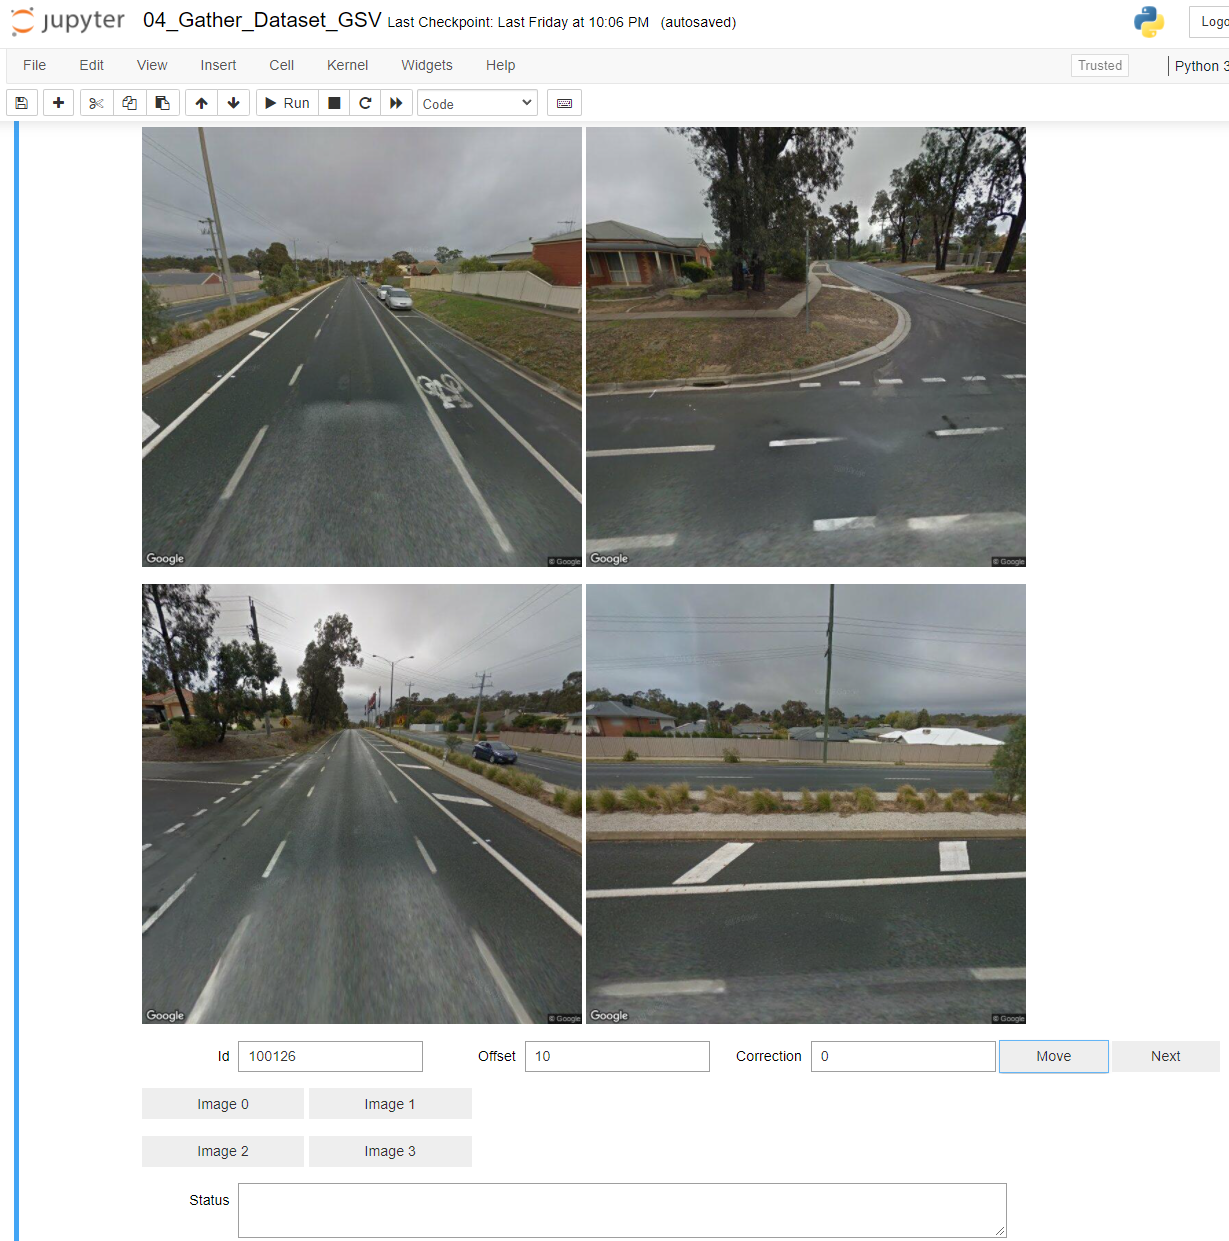
\includegraphics[scale=0.25]{a001_gui.png}
\caption{GUI for gathering Google Street View image dataset}
\label{fig:gui}
\end{figure}

Four images are arranged on screen, with corresponding buttons ``Image 0'' through ``Image 3''.  The top-left image is ``Image 0'' and represents the forward-facing view at the sample location.  The bottom-right is ``Image 2'' and represents the rear-facing view.  The other two images show what appeared alongside the camera vehicle.

The GUI will automatically open with the first randomly-selected sample point.  Examine the four images, and for each image where a bicycle lane marking appears, press the corresponding button to record the ``hit'' in the output CSV ``hits.csv''.  This will mark the image for inclusion in the dataset in the next stage of the process, when images are ``labelled''.  In the example in figure \ref{fig:gui}, a bicycle lane marking is clearly visible in the top-left image, and the operator would hit the ``Image 0'' button to record it.

By default, the ``Offset'' and ``Correction'' text boxes are set to zero.

If you see a bicycle lane marking off in the distance in the forward direction, and you want to move the camera closer to it, enter ``10'' in the ``Offset'' text box, and then press ``Move''.  The ``Status'' box will briefly mention that the next image is being loaded, and then the images will update to a camera position 10 metres down the road.  To move in the reverse direction, enter a negative offset.

Moving forward or backward down the road depends on having the camera set at the correct heading for the road in the first place.  If the camera appears to have been placed so that the ``forward'' direction is at an angle to the road, correct it by entering  a number of degrees in the ``Correction'' text box, and then pressing ``Move''.  The orientation will shift.  Once you are happy the orientation is roughly aligned with the road, you can then enter an offset to move the camera to a better position.

When you are finished trying to obtain sample images from this location, press the ``Next'' button to move to a new sample location.

With practice, multiple sample images can be obtained per minute.  If there is no sign of any bicycle lane marking in the area, even in the distance, then you can quickly skip to the next location by pressing ``Next''.  It is not uncommon for the ``Principal Bicycle Network'' dataset to flag a route in a country town such as Warrnambool as an existing on-road bicycle route, only to find that all Google Street View images appear to show an informal paved shoulder, with no bicycle lane markings anywhere along the road.  If you can see bicycle lane marking in the immediate area, hit a button for each matching image and move on.  If you can see one off in the distance, move the camera 10 or 20 metres to capture it.

Every set of images that is downloaded from Google Street View will be cached in the ``gsv'' directory under ``data\_sources''.

The output of this notebook is a ``hits.csv'' file in ``data\_sources'' containing a list of cached Google Street View images where suitable bicycle lane markings were found.  You can monitor the size of ``hits.csv'' as you go along, to keep track of how many images you have found for your dataset.  Once you have enough images, proceed to notebook 05 for the labelling process.

\subsection{05\_Copy\_GSV\_Images\_For\_Labelling}
\label{aj05}

In notebook 05, we take the Google Street View images previously identified, copy them to a single folder, label them with the ``labelImg'' tool, split them into ``training'' and ``test'' folders.

The key ``Config'' items are a version suffix to give to the dataset, e.g. ``V1'', and the percentage of the dataset that should be held in reserve for ``testing'' of models and not included in the ``training'' data, e.g. ``20'' for 20\%.

Do not run all cells of this notebook at once.  You will need to pause in the middle to run the external ``labelImg'' tool, from \url{https://github.com/tzutalin/labelImg}, or a suitable alternative.

In the first part of the notebook, the code will take every image that was flagged in ``hits.csv'' during the notebook 04 process, and copy them all into a single ``dataset'' folder.

After those cells have run, the notebook will tell you to stop and run the ``labelImg'' tool to ``label'' the data.  This involves telling ``labelImg'' where to find the new ``dataset'' folder with all the images, and then, one image at a time, you draw a bounding box around any object of interest, and give it a label, e.g. ``BikeLaneMarker'' for the bicycle lane markings we are training the model to look for.  See the instructions in the notebook and the official documentation for ``labelImg'' for more details.

Once the labelling is done, you can proceed with running the final cell in the notebook, which will randomly select a percentage of the labelled images in the ``dataset'' file and move them to a ``test'' directory, with the version suffix specified in the ``Config''.  The remainder will be moved to an equivalent ``train'' directory.  The labelled images in the ``train'' and ``test'' directories are ready to be turned into ``tfrecord'' files suitable for TensorFlow processing in the next notebook.


\subsection{06\_Model\_Training\_Setup}
\label{aj06}

The purpose of notebook 06 is to download and compile the required code to support TensorFlow Object Garden development, and to set up ``tfrecord'' files for training and validation of the models.

This notebook is worth running one cell at a time, to watch for errors about missing dependencies, and address them with ``conda install'' or ``pip install'' as required.

Cells 4 and 5 will download the required TensorFlow Object Garden code from GitHub, and then run the required ``protoc'' commands to set it up.

Cell 6 will run a validation script to check that TensorFlow development has been set up correctly.  Not all errors will necessarily mean that the setup is broken, but watch its output to make sure you are not missing any dependencies.

The final two cells will create a ``label map'' file, which must include all the labels that were used in ``labelImg'', and then convert the image and label data in the ``train'' and ``test'' dataset directories into ``tfrecord'' format, for use with TensorFlow.


\subsection{07\_Model\_Training\_GSV}

Notebook 07 allows you to download a pre-trained model from the TensorFlow 2 Object Garden, and configure it for training on the custom dataset.

\url{https://github.com/tensorflow/models/blob/master/research/object_detection/g3doc/tf2_detection_zoo.md}

In our case, we ran this notebook to configure multiple candidate models from the garden, before settling on the ``CenterNet HourGlass104 512x512'' model based on its performance.

In the ``Config'' section, give the URL and Name of the pre-trained model you wish to download, from the table on the above ``TensorFlow 2 Detection Zoo'' webpage.  You can also specify the name you'd like to give to a model when it has been trained and you want to create a ``frozen'' model from it, e.g. ``centernet\_V1''.

Then run the notebook from top to bottom.  The notebook will download the model, and update its configuration to look for our custom objects, instead of the ``COCO 17'' objects it was originally trained to detect.  In the results of the very last cell, it will print three commands that you can run manually, from a command prompt.  It is possible to update the notebook to run the commands from the notebook, but generally you get better, immediate feedback about the progress if you run them yourself from a command prompt.

Run the first command to train the model on our ``train'' dataset for 2000 steps.  Every 100 steps, it will give you statistics how long it is taking to perform each step, on average, and ``loss'' statistics to show how well it thinks it is performing with the ``train'' data.  You can re-run this command with a higher number of training steps to continue the training from where it left off.

The second command allows you to evaluate how the model performs with the ``test'' data that was withheld from training.  It can give you statistics such as ``mean Average Precision'' (mAP) and ``Total Loss''.  How did its predictions compare to the actual labelled bounding boxes in the test data?

The third command allows you to make a smaller ``frozen'' copy of the model.  A ``frozen'' model is useful if you want to:

\begin{itemize}
\item{Keep a smaller copy of the model as-at a certain number of training steps}
\item{Copy the model to a different system where it will be applied}
\end{itemize}

Use notebook 07 to download a pre-trained model and set it up for training, then run the training commands recommended by it until you are happy with the evaluation statistics and think it's ready to apply.  If the model does not perform well, you might need to review the dataset (possibly adding more images) or increase the number of training steps (if that is improving the performance) or switch to a different pre-trained model from the ``zoo''.

The next notebook can help show how the model is performing beyond the statistics, and give insight into what it is struggling with.


\subsection{08\_Apply\_Model\_to\_Train\_and\_Test\_GSV}
\label{a08}

The ``evaluation'' script in notebook 07 will take a model and apply it to the ``test'' data, and produce performance statistics as output.  If you want to \textit{see} how it is performing, notebook 08 can help.  It processes the data from the ``train'' and ``test'' directories, and outputs images that have been sorted into ``hits'' and ``miss'' directories depending on whether a bicycle lane marking was detected, and it will draw a bounding box and confidence score around any detection.

In the ``Config'' section, give it the name of the model, which will either be the ``pretrained\_model\_name'' from notebook 07, or the ``frozen\_name'' if you created a ``frozen'' copy of the model.  Give it the version suffix of the dataset, e.g. ``V1''.  And then the ``confidence threshold'' at which the model should assume that an object has been detected, e.g. ``0.55'' means it will score a ``hit'' if its confidence is 0.55 or greater.

Run it from top to bottom, and it will produce output in \url{detections/train_XXX} and \url{detecions/test_XXX} where \url{XXX} is the version suffix of the dataset.  Within those directories, there will be a \url{hits} folder and a \url{miss} folder, containing output images.  You can review the \url{hits} to see if it accurately placed bounding boxes around the detect objects.  You can review the \url{miss} folder to see the images where it failed to make a detection, where one was expected.  Were there any unusual challenges with the image?  Is it reasonable that the object might not have been clearly visible?  Would it help to add more images like this to the dataset?


\subsection{09\_Filter\_OSM\_to\_Local\_Area}
\label{a09}

Notebooks 01 to 08 prepare and train a model to detect bicycle lane markings.  Next, we need to choose a ``survey area''.  We will use OpenStreetMap data for that area to identify locations to sample -- near each intersection -- and then we will download the images and process them with our model.

The purpose of Notebook 09 is to create a geojson file describing the shape of a local area, such as a town or suburb, based on government-issued data.  We can then use this to extract OpenStreetMap data for that specific area, and use it as our ``survey area''.

In the ``Config'' section, choose a suburb name as the ``locality\_name''.  It will expect to load the government-issued ``LGA\_boundaries\_VIC.geojson'' file from \url{data.gov.au} and reduce it down to a geojson name for the selected suburb.

Download the OpenStreetMap data for Australia from \url{download.geofabrik.de} as instructed in the notebook.

If you run the notebook from top-to-bottom, it will output two suggested ``osmium'' commands.  These are designed to reduce the full ``country-level'' extract of OpenStreetMap data down to data for the survey area.  The first command will reduce the data to the exact official shape of the suburb.  The second command will create an extract for a slightly bigger bounding box, to help identify intersections near the margin on the survey area.

Install the ``osmium'' tool and run the commands suggested by the notebook to create the required OpenStreetMap extracts.


\subsection{10\_Apply\_Model\_to\_Survey\_Area\_GSV\_Images}
\label{a10}

This notebook will identify sample points near intersections in the survey area, download Google Street View images, apply the model, and record any detected bicycle lane markings in the output ``detection\_log.csv''.

If you wish to control Google Street View API costs, please run this notebook one cell at a time.

In the first phase, it will use the OpenStreetMap extracts for the survey area, from notebook 09, to create a list of sample points within a certain number of metres of each intersection.  The ``margin'' parameter lets you specify how many metres either side of each intersection you want to sample.  If it is set to 0, the process will only take samples from the middle of each intersection.  If it is set to 10, it will also take samples 10 metres either side of the intersection.  The recommended setting is 20, because the Australian standards specify that a bicycle lane marking should be within 15 metres of every intersection, and the Google Street View API apparently only gives a distinct image every 10 metres.

At the end of the first phase, the notebook will report how many sample points were identified for margins of 0m, 10m and 20m.  The process will be taking four images per sample point, so multiply the proposed number of sample points by four to get an estimate of the cost.  If there are too many sample points, consider using the ``osmium'' tool with its ``--bbox'' option to extract a smaller rectangular area within the suburb as a sample, instead of processing the whole town.

If you proceed with the rest of the notebook with the proposed sample points, it will download the required images from Google Street View, process them with the model, record the detections to a subdirectory for the ``locality\_name'' within the ``detections'' directory, and create geojson files to be used with the maps in notebook 11.  It will infer detected routes from the detection locations according to some rules, and compare these to what OpenStreetMap said with its ``cycleway'' tags.  As part of the comparison, it will tell you how many metres of bicycle lane routes were detected, how many metres were tagged in OpenStreetMap, how many metres they agree, and how many metres each source had a route that the other one did not.

The ``detections'' folder for the ``locality\_name'' will also have ``hits'' and ``miss'' folders where output images (with bounding box overlays) can be examined.  It can be helpful to quickly flick through the images in the ``miss'' folder to see if there are many clear bicycle lane markings that were missed.  It can also be helpful to flick through the ``hits'' folder to see if there were many false-positives, and what might have been causing them.


\subsection{11\_Map\_Bicycle\_Lanes\_GSV}
\label{a11}

Notebook 11 produces interactive maps to view and compare bicycle lane routes for the survey area:

\begin{itemize}
\item{Map 1 shows each detection as a point on the map}
\item{Map 2 shows the bicycle lane routes that were inferred from the detections}
\item{Map 3 shows bicycle lane routes that are tagged as ``cycleway'' routes in OpenStreetMap}
\item{Map 4 shows a comparison between the detected routes and OpenStreetMap, with different colours to represent where they agree, and where one had a route section that the other did not.}	
\end{itemize}

Set the survey area name in the ``Config'' section, and run the notebook from top to bottom.  You can zoom in and out and pan around each map as required.  The ``Config'' section allows you to set a default zoom level.


\subsection{12\_Split\_Dashcam\_Footage}
\label{a12}

The next group of notebooks are dedicated to detecting bicycle lane routes from dash camera footage instead of Google Street View images.

Notebook 12 expects to find a folder within ``data\_sources'' containing MP4 video files and associated NMEA files.  These came from a ``Navman MiVue 1100 Sensor XL DC Dual Dash Cam'' that records one MP4 video and one NMEA file per minute.

In the ``Config'' section, specify the name of the folder containing the footage, this is effectively the ``survey area''.  You can also specify how many image frames you want to sample, up to the number of frames in the original footage.  E.g. you can reduce 60fps footage down to 5 frames per second.

Run this notebook from top to bottom.  It will split the video files into images on disk, and create a file ``metadata.csv'' with the location for each image based on the NMEA data.

The first progress bar shows how many of the video files have been processed.  Subsequent progress bars show progress through each individual video file as it loads.


\subsection{13\_Copy\_Dashcam\_Images\_For\_Labelling}
\label{a13}

The first time you are processing dashcam footage, it is recommended that you skip straight to notebook 15 and attempt to detect bicycle lane markings with an existing model that was trained with Google Street View images.  That model will not necessarily have ideal performance on the dashcam images, which are taken from a different perspective, with different equipment, at a different resolution.  But running a first pass with the GSV model can help to quickly identify images that could be taken from the dashcam footage and added to the training and validation dataset.

Use notebook 15 to process footage from a ``training'' area.  Then come back to this notebook 13.

In the ``Config'' directory, set the version suffix for the previous GSV dataset that you wish to add to, e.g. ``V1''.  Then set the version suffix for the new dataset version you wish to create e.g. ``V2''.  Then start running the first few cells.

Any ``hits'' from the initial training -- whether they are true positives or false positives -- will be read from the ``detection\_log.csv'' file by notebook 13, and copied to a ``dataset'' folder.

Stop running the notebook, and label the images in the ``dataset'' folder with ``labelImg'' as directed.  To avoid false-positives, it was found to be helpful to label additional classes such as turning arrows, traffic islands, and give way markings, to avoid confusing their simple white markings with bicycle lane markings.  See the notebook instructions for further details.

Once the images in the ``dataset'' directory have been labelled, continue running the notebook.  Existing ``train'' and ``test'' images from the previous dataset will be copied into this new version, according to their original splits.  Then any new images from the dashcam will be split into the ``train'' and ``test'' directories to join them.  Finally, ``tfrecord'' files will be created from them, for TensorFlow to use.


\subsection{14\_Model\_Training\_Dashcam}
\label{a14}

Once new ``train'' and ``test'' datasets have been constructed, with dashcam images supplementing the original Google Street View images, we can train a new model.

This notebook 14 is equivalent to notebook 07, but for the new dataset that includes dashcam images.  We select a pre-trained model that we want to work from, download it, and run the recommended training, evaluation, and model-freezing commands.

Beware that if you give exactly the same ``pretrained\_model\_name'' as you did for GSV training, it will try to continue training that model where you left off.  You may prefer to give a different ``pretrained\_model\_name'' to start the training from scratch.


\subsection{15\_Apply\_Model\_to\_Train\_and\_Test\_Dashcam}
\label{a15}

This notebook 15 is equivalent to notebook 08, but for the new dataset that includes dashcam images.  Run this notebook if you want to visualize the results of applying the model-in-training to the ``train'' and ``test'' datasets.


\subsection{16\_Apply\_Model\_to\_Dashcam\_Footage}
\label{a16}

This notebook 16 is equivalent to notebook 09, instead of sampling Google Street View images near intersections, we are processing every image we extracted from the video footage in notebook 12.

Based on the findings from cycling the ``training area'' footage through notebook 15 -> 13 -> 14 in a loop, some enhancements were made to the model to reduce false positives.  See the notebook and ``Methods'' section of this document for further details.

In the ``Config'' section, you can specify the folder/location being surveyed, and the minimum confidence score required to flag a detection.  Specify the name of the model or frozen model you wish to use, and the dataset version prefix to ensure the correct label map file is used.

The ``mask'' option allows you to specify which part of the frame to run detections on, instead of the whole frame.  This will exclude detections in areas where we do not expect to see a bicycle lane marking, and avoid some potential false positives.  The mask boundary will be drawn on the output images in the ``hits'' and ``miss'' folders, so you can see what was considered by the detection model.

There are some further options to control how many detections are required in a general area before a detection is counted for the purposes of inferring a route.  This is to avoid false positives that occur in a single frame with nothing detected in adjacent frames.  By default, each detection requires two further detections within 50 metres, but a minimum of 10 metres away to avoid duplication when the camera is motionless.

The end result of this notebook is a ``detection\_log.csv'' with all detection points, and ``detection\_log\_filtered.csv'' where one-off detection points that are not supported by nearby detections are excluded.


\subsection{17\_Convert\_Detection\_Log\_to\_GeoJSON}
\label{a17}

In notebook 17, we take the ``detection\_log\_filtered.csv'' output from notebook 16, and correlate it to the OpenStreetMap data, infer bicycle lane routes, map them, and compare to the routes that are tagged as ``cycleway'' in the OpenStreetMap data.  Differences and agreement between routes are measured in metres, and geojson files are created in order to produce maps in the next notebook.

Check the ``Config'' section to make sure the correct dashcam image folder has been specified for the survey area, along with the ``locality'' name for the OpenStreetMap extract.  Then run the notebook from top to bottom.


\subsection{18\_Map\_Bicycle\_Lanes\_Dashcam}
\label{a18}

This notebook 18 is equivalent to notebook 11, except it is producing maps to view and compare routes that were detected from dash camera footage, instead of Google Street View images.

\begin{itemize}
\item{Map 1 shows the bicycle lane routes that were inferred from the detections}
\item{Map 2 shows bicycle lane routes that are tagged as ``cycleway'' routes in OpenStreetMap, where the route was covered by the dash camera footage}
\item{Map 3 shows a comparison between the detected routes and OpenStreetMap, with different colours to represent where they agree, and where one had a route section that the other did not.}	
\end{itemize}


\subsection{19\_Calibrate\_Dashcam}
\label{a19}

The final group of notebooks were used to demonstrate how the general technique of applying a model to images and correlating the result to existing geospatial data could be used to build a dataset about road infrastructure.  In this example, we looked at whether we could detect a ``paved shoulder'' to the left of the camera vehicle's lane, where a cyclist might ride their bike with some separation from other vehicles.  Future work could be looking at estimating lane widths, detecting parked cars or other obstacles in the bicycle lane, or detecting hazardous road surface defects.

Notebook 19 is used to calibrate a model to correct images from the dash camera to account for optical distortion.  Follow the instructions in the notebook (and the reference material linked in the notebook description) to print out a calibration tool that looks like a chessboard.  Record footage of this calibration tool being held up in front of the dash camera at different positions in the frame, at different distances from the camera.

Update the ``Config'' to point to the folder where the calibration videos can be found, and record the number and size of the squares as printed on the calibration tool.  Then run the notebook.

The notebook will split the video into images at 1 frame per second, then follow a standard OpenCV calibration process to produce a model.  The model will then be saved as a ``dashcam\_calibration.yml'' file in the ``data\_sources'' directory.

At the bottom of the notebook, you will see an example of an original image from the dashcam, and a corrected image where the model has been applied to make straight lines appear straighter.


\subsection{20\_Detect\_Paved\_Shoulders\_Dashcam}
\label{a20}

This notebook will re-process the video footage from a survey area, just as notebook 12 did.  But this time:

\begin{itemize}
\item{The model to correct for optical distortion, from notebook 19, will be applied, then...}
\item{A ``lane detection'' model will be applied, to detect the camera's own lane and then the next lane to the left, if any}
\item{The detected lane lines will be overlaid onto output images so that they can be visualized}
\item{For each road segment, from intersection to intersection, an assessment is made as to whether there seems to be a paved shoulder, based on whether one was found in most images, whether it was wide enough, and whether the boundaries were stable enough across the frames in the group.  See the ``Methods'' section and the notebook for further explanation.}	
\end{itemize}

The first significant output of this process is the ``metadata\_with\_summary.csv'' file, which is recorded in the ``split'' subdirectory under the footage folder.  It contains one record per frame, with the summary statistics for the road segment that are used to decide whether there might be a paved shoulder along that segment, or not.

Then, a geojson file is created, to allow us to draw on a map where the paved shoulder detection criteria was met in ``metadata\_with\_summary.csv''.  This is mapped in notebook 21.


\subsection{21\_Map\_Paved\_Shoulders\_Dashcam}
\label{a21}

This notebook draws the detected ``paved shoulders'' from notebook 20 on a map, so that they can be visualized.  Most bicycle lanes should also appear as paved shoulders, so it is useful to compare this output to the other maps in notebooks 18 and 11.


\cleardoublepage
\bibliographystyle{IEEEtran}
\bibliography{Bib/references.bib}
\end{document}}
